\chapter{Theory of Linear Dynamical Systems}\label{chapter:linear_systems}

%-------------------------------------------------
\section{Introduction} %<<<1

%-------------------------------------------------
\subsection{Objectives} %<<<2

	The objective of this chapter is to develop a theory on Linear Dynamical Systems, and particularly, to show that these systems are ``inherently exponential''. Naturally, such theory is highly dependent on Linear Algebra and simple stability definitions, hence why the chapter starts as a Linear Algebra chapter to evolve into Dynamical Systems. This is primarily used as the cornerstone to classical phasors, specifically to show that the differential equations that model Passive Linear Circuits, namely Linear Time Invariant Differential Equations, follow very specific patterns that allow drawing the simple, yet difficult to prove, characteristic that in such circuits the homogeneous solution vanishes exponentially as time grows. This is used in the inception of Classical Phasor Theory, by showing that a PLC when excited by sinusoids experiences sinusoidal responses (voltages and currents) in steady-state because the homogeneous transients fade exponentially.

	The sequence of these facts, however, is not simple to prove. There is a lot of theory regarding Linear Systems and Algebra that need to be undertaken to arrive at the conclusions needed. As such, the objective of this chapter, in a more lengthened explanation, is to introduce the theory of linear systems needed to model and understand Passive Linear Circuits, in a sequence of theorems and developments that, to the best of the author's knowledge, is not found in the literature of Electrical Engineering with the objective of exploring the theory specifically for electrical circuits.

	Furthermore, several constructions and results from this chapter are used in the text. For instance, the definitions of a field and vector space are used in chapter \ref{chapter:dpos} to show that Dynamic Phasor Functionals (the Dynamic Phasor equivalent of derivatives in time domain) form a vector space and a field; also, the same chapter uses the inception of matrices as representations of linear mappings with respect to a particular basis in the definitions of matrices of these Dynamic Phasor Functionals, so that an admittance matrix representation of circuits is possible under nonstationary regimens.

%-------------------------------------------------
\subsection{Notation} %<<<

	Due to the the mathematical-theoretic nature of this thesis, mathematical rigour is needed and with it comes the mathematical notation. The notation used in this thesis is derived from \cite{lamportTLA2002} and \cite{Perko2001}, and is explained as follows.

	The set of natural numbers is denoted $\mathbb{N}$, while the set of integers is $\mathbb{Z}$, the set of real numbers is $\mathbb{R}$ and the complex numbers are $\mathbb{C}$. Complex conjugation is denoted as the overline $\overline{z}$. As in Electrical Engineering the letter ``i'' is generally used for current, we denote the imaginary number that satisfies $x^2 + 1 = 0$ in the complex domain as $j$, and its opposite-conjugate as $\overline{j} = -j$. We consider that zero is a part of the naturals, and $\mathbb{N}_k$ (for a natural $k$) denotes the naturals up to $k$, that is, the set $\left\{0,1,2,...,k\right\}$; conversely, $\mathbb{Z}_k$ represents the integers between and including $-k$ and $k$, that is, $\left\{-k,-(k-1),...,-1,0,1,2,...,k-1,k\right\}$. The sets with superscripts or subscripts represent specific cases: the asterisk $\mathbb{N}^*$ represents a version without zero, the plus sign $\mathbb{R}_+$ represents the non-negative elements (zero is included) and $\mathbb{R}_-$ the non-positive elements.

	Numbers are denoted in simple letters, such as $t$, $x$, and so on. Vectors and matrices are denoted in bold letters: lowercase $\mathbf{x}$ denotes a vector and uppercase $\mathbf{A}$ denotes a matrix. The set of vectors of n dimensions of a particular set $X$ is denoted with a power notation, that is, $X^n$, while the matrices of size n-by-m of $X$ are denoted $X^{(n\times m)}$.  For real and complex numbers, the \textbf{amplitude} or \textbf{absolute value} is denoted with simple vertical brackets as in $\left\lvert a + jb \right\rvert = \sqrt{a^2 + b^2}$. For vectors and matrices the \textbf{norms} are denotes using double vertical bars, as in $\left\lVert \mathbf{x}\right\rVert$ and $\left\lVert \mathbf{A}\right\rVert$. Unless specifically noted, the vector and matrix norms are the $p$-norm for an arbitrary $p$. This will be defined thoroughly in the text.

	Matrix simple transposition is denoted with a stylized ``T'', as in, $\mathbf{A}^\transpose$, and the hermitian transpose (conjugate transpose) is denoted with a stylized ``H'' as in $\mathbf{A}^\hermconj$
.

	An \textbf{application}, or mapping, is a set-theoretic relationship that maps elements from a domain $D$ (denoted $D = \Dom\left(f\right)$) and assumes values in a certain other set $T$, denoted in simple letters with a bracket as in $f\left[x\right]$. The collection of all possible outputs of $f$ is called the image of $f$, denoted $\Im\left(f\right)$, defined as

\begin{equation} \Im\left(f\right) = \left\{ f\left[x\right]: x\in\Dom\left(f\right)\right\}. \label{eq:def_image}\end{equation}

	If the argument $x$ does not belong to $D$ then $f$ applied to $x$ is unspecified. A \textbf{function} is a mapping such that $f\left[x\right]$ is unique to $x$ (that is, a certain $x$ can only have one $f\left[x\right]$) while the converse is not necessarily true; if it is (that is, each $x$ maps uniquely to $f\left[x\right]$) then $f$ is called \textit{injective}. Naturally, $\Im\left(f\right)\subset T$; if equality holds, $f$ is called \textit{surjective}. A function that is both inective and surjective is such that an element of $\Dom\left(f\right)$ is biunivocally related to another element (``one-to-one'') in the image, and this image spans the entire space in which $f$ takes values; such a function is called \textit{bijective}. Many equivalent definitions for injections, surjections and bijections exist, and any book on analysis will present a definition that suits its text.

	 In most cases it is convenient to associate to $f$ some expression $e(x)$ such that $f\left[x\right] = e(x)$ (note that the brackets denote a function while the parenthesis denote a syntax). In this case, $f$ is defined as $f\coloneq \left[x\in D\mapsto e(x)\right]$, the symbol ``$\coloneq$'' denoting a definition. In this definition, the target set $T$ is supposed to be the largest one where the expression $e(x)$ takes values on. It might be interesting to state and define $D$, $T$ and $e(x)$ clearly; in this case, the longer notation

\begin{equation} f: \left\{\begin{array}{rcl} D &\to& T \\[3mm] x &\mapsto& e(x) \end{array}\right. \end{equation}

	\noindent is used. The notation $\left[D\to T\right]$ denotes the \textbf{set of all functions} from the set $D$ that take value in the set $T$, such that $f\in\left[D\to T\right]$ reads ``$f$ is a function with domain $D$ that takes values in a set $T$''. Particularly, functions of real numbers are called \textbf{signals}, that is, $f\in\left[\mathbb{R}\to X\right]$ is a signal onto the set $X$; $\left[\mathbb{R}\to\mathbb{R}\right]$ are the \textbf{real signals} and $\left[\mathbb{R}\to\mathbb{C}\right]$ are the \textbf{complex signals}. In general, signals are called so to represent quantities that vary in time, that is, most signals are functions of time.

	A function is called a \textbf{transform} if it is a self-map, that is, takes elements from a domain $X$ into $X$ itself. Indeed, the usual functional transforms (Fourier, Laplace, Hilbert and so on) transform complex signals into complex signals.

	A \textbf{sequence} is a function from either the naturals or the integers. The notation $X^{\left[\mathbb{N}\right]}$ denotes a natural sequence in a set $X$, that is, an ennumerated collection $A = \left(a_0,a_1,a_2,...\right)$ such that all $a_k\in X$. This can be shortly denoted as $A = \left(a_k\right)_{k=0}^\infty$. In the same way, $X^{\left[\mathbb{Z}\right]}$ denotes an integer sequence in $X$, that is, an ordered set $A = \left(...,a_{(-2)},a_{(-1)},a_0,a_1,a_2,a_3,...\right)$ with all $a_k\in X$, which can be deonted in short as $A = \left(a_k\right)_{k\in\mathbb{Z}}$. In some cases it might be interesting to have finite sequences — also called \textbf{tuples} — say, from index 0 to a finite index $m$, which can be denoted $\left(a_k\right)_{k=0}^m$. It must be noted that sequences, by being ennumerated collections, define unique relations with respect to their elements, that is, a sequence $A$ is only equal to a sequence $B$ if $a_k = b_k$ for all indexes $k$.

	\textbf{Operators and functionals} are maps defined in spaces of functions, that is, ``functions of functions'', and are denoted with brackets and in bold letters. \textbf{Operators} are denoted in lowercase bold letters with brackets and transform functions into numbers; for instance, the norm of a function in the Banach $L^2$ space is defined as

\begin{equation} \mathbf{n}_2\left[\cdot\right] : \left\{\begin{array}{rcl} L^2\left(\mathbb{R}\right) &\to& \mathbb{R}^+ \\[3mm] f(x) &\mapsto& \sqrt{\raisebox{0mm}[7mm][6mm]{} \displaystyle\int_{-\infty}^{\infty} f(x)^2 dx}\end{array}\right.  .\end{equation}

	Sometimes, however, some special operators have specific notations; for instance, norms are generally noted in vertical brackets like $\left\lVert f \right\rVert_2$. \textbf{Functionals}, on the other hand, deliver functions into functions, and are denoted in uppercase bold letters; for instance, the Laplace Transform of a function $f$ is denoted $\mathbf{L}\left[f\right]$, the Fourier Transform $\mathbf{F}\left[f\right]$, the Hilbert Transform $\mathbf{H}\left[f\right]$ and so on. It is on purpose that both matrices and functionals are denoted in uppercase bold, for the multiplication of a matrix $\mathbf{A}$ and a vector function $\mathbf{x}(t)$ is a linear functional $\mathbf{A}\left[\mathbf{x}\right]$, while any linear functional can be expressed as a matrix given some basis.

	It must be noted that the distinction between operators, functionals and transforms made here is not standardized in mathematics and may vary among the literature and authors.

	Derivatives are noted with apostrophes, as in, $f'(x)$ represents the first derivative, $f''(x)$ represents the second, $f'''(t)$ represets the third and so on. Particularly for time derivatives, the over-dot notation $\dot{f}(t), \ddot{f}(t), \dddot{f}(t)$ is used. For higher-order or generic-order derivatives, the exponent with parenthesis $f^{(n)}$ is used. Differentials, on the other hand, are denoted in two ways: either as functionals or in the ``fraction-like'' Leibnitz notation. For the first notation, the usual $d$ is used for single-variable functions:

\begin{equation} \dfrac{df(x)}{dx} \text{, for the first derivative and } \dfrac{d^nf(x)}{dx^n} \text{ for the n-th order} .\end{equation}

%	\noindent while the \textit{del} $\partial$ is used for multivariate functions
%
%\begin{equation} \begin{array}{l} \dfrac{\partial f(\mathbf{x})}{\partial x_k} \text{ for the first derivative with respect to the k-th coordinate} \\[5mm] \dfrac{\partial^n f(\mathbf{x})}{\partial x_k^n} \text{ for the n-th derivative with respect to the k-th coordinate, and } \\[5mm] \dfrac{\partial^n f(\mathbf{x})}{\partial x_1\partial x_2 \cdots \partial x_k} \text{ for mixed or sequential derivatives} \end{array} \end{equation}

	For normed vector spaces, and particularly Banach Spaces such as functional spaces, the delta $\delta$ is used to denote the Frechèt derivative as in

\begin{equation} \left.\dfrac{\delta \mathbf{F}\left[x\right]}{\delta x}\right\rvert_{x=x_0} \end{equation}

	\noindent denotes the derivative of the functional $F$ with respect to $x$ calculated at $x_0$. This derivative is defined as the bounded linear map $\mathbf{A}$ that satisfies

\begin{equation} \mathbf{A} = \left.\dfrac{\delta \mathbf{F}\left[x\right]}{\delta x}\right\rvert_{x=x_0} \Leftrightarrow \lim\limits_{\left\lVert \Delta x\right\rVert\to 0} \dfrac{\left\lVert \mathbf{F}\left[x_0 + \Delta x\right] - \mathbf{F}\left[x_0\right] - \mathbf{A}\left[x_0\right] \Delta x \right\rVert_W}{\left\lVert \Delta x\right\rVert_V} = 0 \label{eq:def_frechet}\end{equation}

	\noindent called the Frechèt Derivative \pcite{gelfandCalculusVariations1963}, where $\mathbf{A}\left[x\right] \Delta x$ is $\mathbf{A}$ calculated at the operating point $x_0$ applied onto $\Delta x$. It is obvious that $\mathbf{A}$ depends on the point $x_0$ it is calculated against; yet, the notation $\mathbf{A}\left[x_0\right]$ denotes the operator \textit{calculated at} $x_0$ and not operating on it, which can become confusing. Thus, the shorter notation $\mathbf{A}$ will be used when $x_0$ is understood while the fraction notation will be used to highlight the operating element. It is also obvious that this definition depends on the specific norms adopted for the domain space $\left\lVert\cdot\right\rVert_V$ and the image space $\left\lVert\cdot\right\rVert_W$; in most cases these norms are tacitly understood.

	For the differential operators notation, the small caps bold $\mathbf{d}$ is used. For sequential differentiation, $\mathbf{d}^k$ denotes the k-th order differential operator. Because the differentiation operation varies in definition among the many sets involved, generally the functional will be noted with a subscript. For instance, the differentiation of real signals is the operator that takes a function and an operating point and delivers the derivative of that function at that point

\begin{equation}\mathbf{d}_\mathbb{R}: \left\{\begin{array}{rcl} \mathbb{R}\times\left[\mathbb{R}\to\mathbb{R}\right] &\to& \mathbb{R} \\[3mm] \left(x_0,f(x)\right) &\mapsto& \left.\dfrac{df(x)}{dx}\right\rvert_{x=x_0} \end{array}\right.\end{equation}

	\noindent and when the operating point $x_0$ is understood, the shorter notation $f'(t)$ is used. At the same time, the differentiation of complex signals is

\begin{equation}\mathbf{d}_\mathbb{C}: \left\{\begin{array}{ccc} \mathbb{R}\times\left[\mathbb{R} \to\mathbb{C}\right] &\to& \mathbb{C} \\[3mm] \left(x_0,u(x) + jv(x)\right) &\mapsto& \mathbf{d}_\mathbb{R}\left[x_0,u\right] + j \mathbf{d}_\mathbb{R}\left[x_0,v\right]\end{array}\right.\end{equation}

	\noindent and so on. From these definitions one can define differential functionals, denoted in uppercase bold, where the differential operators are evaluated continuously, as in

\begin{equation}\mathbf{D}_\mathbb{R}: \left\{\begin{array}{rcl} \left[\mathbb{R}\to\mathbb{R}\right] &\to& \left[\mathbb{R}\to\mathbb{R}\right] \\[3mm] f(x) &\mapsto& f'(t) = \mathbf{d}_\mathbb{R}\left[t,f\right] \end{array}\right.\end{equation}

	\noindent and, conversely,

\begin{equation}\mathbf{D}_\mathbb{C}: \left\{\begin{array}{ccc} \left[\mathbb{R} \to\mathbb{C}\right] &\to& \left[\mathbb{R}\to\mathbb{C}\right] \\[3mm] f(t) = u(x) + jv(x) &\mapsto& f'(t) = \mathbf{d}_\mathbb{R}\left[t,u\right] + j \mathbf{d}_\mathbb{R}\left[t,v\right]\end{array}\right.\end{equation}

	Finally, given a function $f\in\left[X\to Y\right]$ and the differential operator, $f$ is said to be \textbf{class n smooth at} $x_0$ if $\mathbf{d}^n\left[x_0,f\right]$ exists. Conversely, defining a functional $\mathbf{D}_X$ of the space $X$, then $f$ is said to be \textbf{class n smooth} if $\mathbf{D}^n\left[f\right]$ exists in $X$. The set of class n smooth functions in $X$ is denoted $C_X^n$ (or simply $C^n$ when $X$ and $\mathbf{D}_X$ are tacitly understood), so that $f\in C^n$ reads ``$f$ is class $n$ smooth''.

%-------------------------------------------------
\section{Linear Circuits as Linear Functionals} %<<<1

	The theory of linear operators is generally defined in terms of vector fields and scalars, which is explained swiftly below.

\begin{definition}[Field]\label{def:field}
	A \textbf{field} is a set $F$ wherein two binary operations are defined: the sum ``$+$'' and multiplication ``$\cdot$'', following certain rules:

\begin{itemize}
	\item \textbf{Associativity}: for three $a,b,c$ in $F$, $a+(b+c) = (a+b)+c$ and $a\cdot (b\cdot c) = (a\cdot b) \cdot c$;
	\item \textbf{Commutativity}: for any $a,b$ in $F$, $a+b = b+a$ and $a\cdot b = b\cdot a$;
	\item \textbf{Identities}: there exist two elements in $F$, 0 and 1, such that $a + 0 = a$ and $a\cdot 1 = a$ for all $a\in F$;
	\item \textbf{Additive inverse}: for any $a\in F$, there exists the additive inverse $-a$ such that $a + (-a) = 0$ ;
	\item \textbf{Multiplicative inverse}: for any $a\in F$ except $0$ there exists the multiplicative inverse $a^{-1}$ such that $a\cdot a^{-1} = 1$ ;
	\item \textbf{Distributivity} of multiplication over sum: for $a,b,c\in F$, $a\cdot (b + c) = a\cdot b + a\cdot c$.
\end{itemize}
\end{definition}

	Classically, in linear algebra the field of reals and complex numbers is used; it is simple to prove that the usual complex sum and multiplication adhere to the properties of fields. Concurrently, one can define the notion of a vector space.

\begin{definition}[Vector space]\label{def:vector_space}%<<<
	A \textbf{vector space} $V$ over a field $F$ is a set wherein two binary operations can be defined: vector sum, or simply sum, and scalar multiplication. In this thesis, vectors are denoted in boldface to distinguish them from the elements of the field $F$, called scalars. These operations again have certain properties

\begin{itemize}
	\item \textbf{Associativity}: for three $\mathbf{u,v,w}$ in $V$, $\mathbf{u+(v+w)} = \mathbf{(u+v)+w}$;
	\item \textbf{Commutativity}: for any $\mathbf{u,v}$ in $V$, $\mathbf{u+v=v+u}$;
	\item \textbf{Identity of vector sum}: there exists an element called the zero vector $\mathbf{0}$ in $V$ such that $\mathbf{v+0 = 0}$ for all $\mathbf{v}\in V$;
	\item \textbf{Additive inverse}: for any $\mathbf{v}\in V$, there exists the additive inverse $-\mathbf{v}$ such that $\mathbf{v + (-v) = 0}$ ;
	\item \textbf{Scalar multiplication compatibility}: for any two scalars $a,b\in F$ and any vector $\mathbf{v}\in V$, $a(b\mathbf{v}) = (ab)\mathbf{v}$ ;
	\item \textbf{Identity element of scalar multiplication}: there exists an element $1\in F$ such that $1\cdot \mathbf{v} = \mathbf{v}$ for any $\mathbf{v}\in V$ ;
	\item \textbf{Distributivity}: for any two scalars $a,b$ and two vectors $\mathbf{v,u}$, $a\mathbf{v} + b\mathbf{v} = (a+b)\mathbf{v}$ and $a(\mathbf{v+u}) = a\mathbf{v} + b\mathbf{u}$.
\end{itemize}
\end{definition}

	Although the definitions seem somewhat prolix or tedious, the reach of these definitions is immense. In general, the most common vector space is the space of complex vectors of length $n$, denoted $\mathbb{C}^n$, that is, numbers of the form $\mathbf{z} = \left[z_1,z_2,...,z_n\right]^\transpose$ where all $z_k$ are complex numbers, or particularly, the space of real vectors of length $n$. It is immediate to notice that $\mathbb{C}^n$ and $\mathbb{R}^n$ are vector fields over their unidimensional counterparts, and a introductory level in linear algebra will deal in such realms.

	It is however, less obvious to notice that the space $\left[\mathbb{R}\to\mathbb{C}^n\right]$ of complex vector functions of one real variable of length $n$ a vector space over the field of complex numbers. Indeed, by adopting the vector sum operation as

\begin{equation} (+): \left\{\begin{array}{rcl} \left[\mathbb{R}\to\mathbb{C}^n\right]^2 &\to& \left[\mathbb{R}\to\mathbb{C}^n\right] \\[5mm] \left(\left[\begin{array}{c} x_1\left(t\right) \\[3mm] x_2(t) \\[3mm] \vdots \\[3mm] x_n(t) \end{array}\right],\left[\begin{array}{c} y_1\left(t\right) \\[3mm] y_2(t) \\[3mm] \vdots \\[3mm] y_n(t) \end{array}\right]\right) &\mapsto& \left[\begin{array}{c} x_1\left(t\right) + y_1\left(t\right) \\[3mm] x_2\left(t\right) + y_2\left(t\right) \\[3mm] \vdots \\[3mm] x_n\left(t\right) + y_n\left(t\right) \end{array}\right] \end{array}\right. \end{equation}

	\noindent and the scalar multiplication as

\begin{equation} (\cdot): \left\{\begin{array}{rcl} \mathbb{C}\times\left[\mathbb{R}\to\mathbb{C}^n\right] &\to& \left[\mathbb{R}\to\mathbb{C}^n\right] \\[5mm] \left(z,\left[\begin{array}{c} x_1\left(t\right) \\[3mm] x_2(t) \\[3mm] \vdots \\[3mm] x_n(t) \end{array}\right]\right) &\mapsto& \left[\begin{array}{c} zx_1\left(t\right) \\[3mm] zx_2\left(t\right) \\[3mm] \vdots \\[3mm] zx_n\left(t\right) \end{array}\right] \end{array}\right. \end{equation}

	\noindent then one can prove that these operations fulfill of the definitions of a vector space over a field. A function $\alpha$ defined from a vector space to another vector space maintaining the linear structure is called a \textbf{linear map}. More precisely, for two vector spaces $V$ and $U$, $\alpha \in\left[V\to U\right]$ is a linear operator if $\alpha\left(\mathbf{x} + \mathbf{y}\right) = \alpha\mathbf{x} + \alpha\mathbf{y}$  for any two $\mathbf{x,y}\in V$ and $\alpha\left(z\mathbf{x}\right) = z\alpha\left(\mathbf{x}\right)$ for any scalar $z$ and any vector $\mathbf{x}\in V$.  In this thesis, the two vector spaces of interest are either $\left[\mathbb{R}\to\mathbb{C}^n\right]$ or $\mathbb{C}^n$, both over $\mathbb{C}$. 

	For the purposes of electrical circuits analysis and electrical network theory, linear circuits — circuits composed of resistances, inductances and capacitances — are generally modelled as differential equations of the form

\begin{equation} \dot{\mathbf{x}}(t) = \mathbf{A}\left[\mathbf{x}\right](t) + \mathbf{f}(t), \label{eq:matrix_lti_ode_eq_def} \end{equation}

	\noindent where $\mathbf{A}\left[\mathbf{x}\right]$ is a transform in the space $\left[\mathbb{R}\to\mathbb{C}^n\right]$. Additionally, $\mathbf{A}\left[\cdot\right]$ is \textit{linear}, that is,

\begin{equation} \mathbf{A}\left[\mathbf{x} + \alpha\mathbf{y}\right] = \mathbf{A}\left[\mathbf{x}\right] + \alpha\mathbf{A}\left[\mathbf{y}\right] \end{equation}

	\noindent for any $\mathbf{x,y}\in\left[\mathbb{R}\to\mathbb{C}^n\right]$ and $\alpha$ a scalar.

	The fact that a linear circuit can indeed be modelled as an equation of the form \eqref{eq:matrix_lti_ode_eq_def} will be shown in section \ref{chapter:classical_phasors}, hence this fact is for now assumed. In such circuits, the coefficients $a_{ik}$ are certain combinations of the $RLC$ parameters of the circuit derived by manipulating and modelling the circuit using Kirchoff's Laws.

	As for nomenclature, $\mathbf{x}(t)\in\left[\mathbb{R}\to\mathbb{C}^n\right]$ is the system \textbf{output} or \textbf{response}, and $\mathbf{f}(t)\in\left[\mathbb{R}\to\mathbb{C}^n\right]$ is some \textbf{forcing, excitation} or \textbf{input}. An equation in the form of \eqref{eq:matrix_lti_ode_eq_def} is described as the \textbf{state-space equation} of the system, where the components of $\mathbf{x}$ are called \textbf{states}. Loosely, states are certain quantities within the system such that \textit{their collection suffices to describe the system completely}, as in, any other quantity can be obtained from the states. For linear circuits, it will be proven in section \ref{chapter:classical_phasors} that inductor currents and capacitor voltages are states of the system for any node voltage or branch current is obtainable from this list. More precisely, suppose that the system has $n$ nodes and $b$ branches and adopt

\begin{equation} \mathbf{v} = \left[ \overbrace{v_1,v_2,...,v_n}^{\text{Node voltages}}\right],\mathbf{i} = \left[ \overbrace{i_1, i_2 , ... i_b}^{\text{Branch currents}}\right]^\transpose .\end{equation}

	Now suppose the circuit has $q$ capacitors and $p$ inductors. Then the sate vector is

\begin{equation} \mathbf{x} = \left[ \overbrace{v_{C_1},v_{C_2},...,v_{C_q}}^{\text{Capacitor voltages}}, \overbrace{i_{L_1}, i_{L_2} , ... i_{L_p}}^{\text{Inductor currents}}\right]^\transpose .\end{equation}

	\noindent then $\mathbf{v}$ and $\mathbf{i}$ can be obtained as some linear combinations of $\dot{\mathbf{x}}$ and $\mathbf{x}$ . The converse is also true as a direct consequence of Kirchoff's Laws.

%	And there exist two matrices $\mathbf{N,M}$ such that 
%
%\begin{equation} \left[\begin{array}{c} \mathbf{v} \\[3mm] \mathbf{i} \end{array}\right] = \mathbf{N}\dot{\mathbf{x}} + \mathbf{Mx} . \end{equation}
%	
%	The converse is also true as a direct consequence of Kirchoff's Laws, that is, there exists a matrix $\mathbf{P}$ such that 

%\begin{equation} \mathbf{x} = \mathbf{P} \left[\begin{array}{c} \mathbf{v} \\[3mm] \mathbf{i} \end{array}\right] . \end{equation}


\begin{example}\label{example:rlc_circuit_lti_ode_example} % EXAMPLE OF LTI ODE CIRCUIT MODELLING <<<
	Consider the figure \ref{fig:ltiode_modelling_example_circuit} where an RLC circuit is shown. This circuit has an excitation $u(t)$, given by a controlled voltage source, and an input $v(t)$, given by the voltage across the resistor load $R$. The circuit has two nodes and two loops are shown, a red and a green one.

% MODELLING EXAMPLE: RLC CIRCUIT <<<
\begin{figure}[htb!]
\centering
\scalebox{0.75}{
        \begin{tikzpicture}[american,scale=1.2,transform shape,line width=0.75, cute inductors]
		\draw (0,0)
			to[vsource,sources/scale=1.25, v>=$u(t)$,invert] (0,4)
			to[L,l=$L$,f>^=$i_L$,v>=$v_L(t)$,-*] (4,4) 
			to[C, l_=$C$,f>_=$i_C$, v^=$v_C(t)$, voltage shift = 0.5mm] (4,0)
			to[short] (0,0); 
		\node[shape=circle,draw,inner sep=1pt] at (4,4.5) {$1$};
		\draw (4,4) to[short] (5,4) to[short] (8,4) to[R,l_=$R$,f>_=$i_R$, v^=$v(t)$,voltage shift = 1mm] (8,0) to[short] (4,0);
		\draw[rounded corners=10,loop, draw opacity=0.3,->,color=red] (0.5,0.5) -- (0.5,3.5) -- (3.5,3.5) -- (3.5,0.5) -- (1,0.5) ;
		\draw[rounded corners=10,loop, draw opacity=0.3,->, color=blue] (4.5,0.5) -- (4.5,3.5) -- (7.5,3.5) -- (7.5,0.5) -- (5,0.5) ;
        \end{tikzpicture}
}
	\caption{RLC circuit as modelling example for linear circuit as an LTI ODE.}
	\label{fig:ltiode_modelling_example_circuit}
\end{figure} %>>>

	First, apply the KVL to the red loop and blue loops to yield

\begin{equation}
	\left\{\begin{array}{l}
		-u(t) + v_L(t) + v_C(t) = 0 \\[3mm]
		-v_C(t) + v(t) = 0
	\end{array}\right. \label{fig:ltiode_modelling_example_circuit_kvl}
\end{equation}

	Then apply the KCL to the node $1$:

\begin{equation} i_L(t) - i_C(t) - i_R(t) = 0 \label{fig:ltiode_modelling_example_circuit_kcl} \end{equation}

	Therefore, equations \eqref{fig:ltiode_modelling_example_circuit_kvl} and \eqref{fig:ltiode_modelling_example_circuit_kcl} form a three-equation system with six states $v_C,v_L,v,i_R,i_C,i_L$. The remaning three equations come from the equations of the circuit elements:

\begin{equation}
	\left\{\begin{array}{l}
		i_R(t) = Rv(t) \\[3mm]
		i_C(t) = C \dfrac{dv_C(t)}{dt} \\[3mm]
		v_L(t) = L\dfrac{di_L(t)}{dt}
	\end{array}\right. \label{fig:ltiode_modelling_example_circuit_components}
\end{equation}

	Now let

\begin{equation} \mathbf{x} = \left[\begin{array}{c} v_C \\[3mm] i_L \end{array}\right] \end{equation}

	Then the first equation of \eqref{fig:ltiode_modelling_example_circuit_kvl} and \eqref{fig:ltiode_modelling_example_circuit_kcl} yield

\begin{equation} \left\{ \begin{array}{l} \dot{v}_C = \dfrac{1}{C} \left(i_L - \dfrac{v_C}{R}\right) = -\dfrac{1}{RC}v_c + \dfrac{1}{C}i_L \\[5mm] \dot{i}_L = \dfrac{1}{L} \left(u - v_C\right) = - \dfrac{1}{L}v_C + \dfrac{1}{L}u \end{array}\right.\end{equation}

	\noindent meaning this circuit is such that

\begin{equation} \mathbf{A}\left[ \begin{array}{l} v_C \\[3mm] i_L \end{array}\right] = \left[\begin{array}{c} -\dfrac{1}{RC}v_c + \dfrac{1}{C}i_L \\[5mm] - \dfrac{1}{L}v_C \end{array}\right]\end{equation}

	\noindent which is clearly linear, thus this circuit defines an equation like \eqref{eq:matrix_lti_ode_eq_def}.

\examplebar
\end{example} %>>>

	In general, the objective of discussions of differential equations in applied sciences is to \textbf{solve} the equation, that is, find a \textbf{solution} to \eqref{eq:matrix_lti_ode_eq_def} — a particular signal $\mathbf{x}(t)$ that satisfies the equation given a set of initial conditions $\mathbf{x}\left(t_0\right),\mathbf{x}'\left(t_0\right),...,\mathbf{x}^{(n-1)}\left(t_0\right)$ for some time $t_0$. Such a process is called \textbf{solving} or \textbf{integrating} the differential equation. In most cases, a introductory Differential Equations course is concerned with teaching algorithms and techniques to solve differential equations analytically; in this text, it is assumed the reader is acquainted with such processes. Here we are more interested with the fact that, in a deeper sense, solving \eqref{eq:matrix_lti_ode_eq_def} is equivalent to finding the root of the functional equation

\begin{equation} \mathbf{D}_{\mathbb{C}^n}\left[\mathbf{x}\right] - \mathbf{A}\left[\mathbf{x}\right] = \mathbf{f}(t),  \label{eq:equivalent_lti_ode_operator} \end{equation}

	\noindent where $\mathbf{D}_{\mathbb{C}^n}$ denotes the differential functional in $\mathbb{C}^n$.  Ideally, one can find the set of all solutions, that is, an expression that defines the entire class of functions that solve the equation. Such expression is known as the \textbf{general solution}. 

% which will be described in the form of a n-th order differential equation
%
%\begin{equation} \sum\limits_{k=0}^n \alpha_k x^{\left(k\right)} - {f}(t) = 0, \label{eq:vector_lti_ode_eq_def} \end{equation}
%
%	\noindent where the $\alpha_k$ are complex numbers with $\alpha_n\neq 0$, $x\in\left[\mathbb{R}\to\mathbb{C}\right]$ and ${f}(t)\in\left[\mathbb{R}\to\mathbb{C}\right]$ output and input respectively. The difference between the matrix equation \eqref{eq:matrix_lti_ode_eq_def} and the n-th order equation \eqref{eq:vector_lti_ode_eq_def} is a practical one, because mathematically, \eqref{eq:vector_lti_ode_eq_def} are special cases of matrix ODE where a vector form is equivalent to a space-state equation on $n$ states. Indeed, write
%
%\begin{equation} \mathbf{x} = \left[\begin{array}{c} x(t) \\[3mm] x^{(1)}(t)\\[3mm] x^{(2)}(t) \\[3mm] \vdots \\[3mm] x^{(n-1)} (t) \end{array}\right] \end{equation}
%
%	\noindent and \eqref{eq:vector_lti_ode_eq_def} is equivalent to the matrix LTI ODE
%
%\begin{equation} \dot{\mathbf{x}} = \mathbf{A}\mathbf{x} \label{eq:theo_matrix_equivalence_matrix_ode} \end{equation}
%
%	\noindent where
%
%\begin{equation} \mathbf{A} = \left[\begin{array}{ccccc} 0 & 1 & 0 & ... & 0 \\[3mm] 0 & 0 & 1 & ... & 0  \\[3mm] \vdots & \vdots & \vdots & \ddots & \vdots \\[3mm] 0 & 0 & 0 & ... & 1 \\[3mm] -\dfrac{\alpha_0}{\alpha_n} & -\dfrac{\alpha_1}{\alpha_n} & -\dfrac{\alpha_2}{\alpha_n} & ... & -\dfrac{\alpha_{(n-1)}}{\alpha_n} \end{array}\right] \label{eq:equivalent_frobenius_matrix}\end{equation}
%
%	For engineers, however, the n-th order differential form is easier to work with because they are also somewhat easier to solve: it will be shown that its solutions can be found through the polynomial
%
%\begin{equation} H(x) = \sum\limits_{k=0}^n \alpha_k x^k \end{equation}
%
%	\noindent which is easily obtained by substituting the derivative orders of the original ODE \eqref{eq:vector_lti_ode_eq_def} into exponents. Albeit both forms being somewhat equivalent, however, the state-space form is easier to work with in a proof context because its qualitative and quantitative behavior can be drawn as direct consequences of the matrix $\mathbf{A}$ and its characteristics, specifically its eigenvectors and eigenvalues. Therefore, in what follows, the theorems and proofs will be shown for the state-space form \eqref{eq:matrix_lti_ode_eq_def} and then particularized for the n-dimensional case later

	The nomenclature of ``linear`` and ``time invariant`` for \eqref{eq:matrix_lti_ode_eq_def} comes from the ability to combine inputs and predict the outputs basisd on the individual response of each input. Let 

\begin{equation} \mathbf{G}\left[\mathbf{f}\right] = \mathbf{x}(t) , \label{eq:lti_system_def} \end{equation}

	\noindent be a shorthand notation (generally called ``input-output notation'') for the differential equation \eqref{eq:matrix_lti_ode_eq_def}, and reads ``the system $\mathbf{G}$ maps the input $\mathbf{f}$ to the output $\mathbf{x}$''. Note that $\mathbf{G}\left[\cdot\right]$ relates a function $\mathbf{f}$ to another function $\mathbf{x}$, thence $\mathbf{G}\left[\cdot\right]$ is a functional. Exploring the properties of \eqref{eq:matrix_lti_ode_eq_def} we prove that $\mathbf{G}$ is \textbf{linear}, that is, a linear combination of inputs is equivalent to the same linear combination of responses:
	
\begin{equation} \mathbf{G}\left[\mathbf{f}_1 + \alpha\mathbf{f}_2\right] = \mathbf{G}\left[\mathbf{f}_1\right] + \alpha\mathbf{G}\left[\mathbf{f}_2\right],\ \alpha\in\mathbb{C} \label{eq:lti_scaling}.\end{equation}

	The map $\mathbf{G}$ is also \textbf{time invariant}, because a delay $\tau$ in the input causes a delay $\tau$ in the output:

\begin{equation} \mathbf{G}\left[\mathbf{f}\left(t - \tau\right)\right] = \mathbf{x}\left(t-\tau\right) \label{eq:lti_delay}\end{equation}

	These properties are easily drawn from the linearity of the operator $\mathbf{A}$ and the time invariancy of the derivative operator. Therefore, a state-space equation of the form $\dot{\mathbf{x}} = \mathbf{Ax} + \mathbf{f}\left(t\right)$ is called a \textbf{Linear Time Invariant} system, or LTI for short. Linearity and time invariancy are rather intuitive concepts: linear systems are those that follow the superposition principle — meaning superposing inputs is equivalent to superposing their respective outputs — whereas time invariant systems are ones that do not ``change in time'' or do not ``age'', that is, the input-to-output mapping does not change as time grows, such that the same input applied at a delay will yield the same output, only delayed by the same amount.

	With clarity in the best interest, and because this thesis is concerned only with systems of the form \eqref{eq:matrix_lti_ode_eq_def}, these LTI systems will be thenceforth called simply \textbf{linear systems}.
	
\begin{example}\label{example:rlc_circuit_lti_ode_example} % EXAMPLE OF LTI ODE CIRCUIT MODELLING <<<
	Consider again the figure \ref{fig:ltiode_modelling_example_circuit} and adopt  $L = 10$mH, $C = 1\mu$F and $R = 1$k$\Omega$. Suppose the system is subject to three different excitations: $u_1(t) = \theta\left(t\right)$, $u_2(t) = \theta\left(t-5ms\right)$ and $u_3(t) = 2\theta\left(t\right)$ with $\theta(t)$ the heaviside step function. That is, $u_2$ and $u_3$ are identical to $u_1$, except $u_2$ is a delayed version with a delay of 5 miliseconds and $u_3$ is scaled by a factor of two. Figure \ref{fig:delayed_example_rlc_ltiode} shows the system load voltage response $v(t)$ to all three excitations, and it is clear that the responses $v_2(t)$ and $v_3(t)$ are copies of $v_1$, albeit $v_2$ being delayed by the same 5 miliseconds and $v_3$ scaled by the same factor of two. This shows that, indeed, the circuit is linear and time-invariant system: a scaling of input caused the same scaling of output, and a delay in the input caused the same delay in the output.

% TIME INVARIANCY PLOT EXAMPLE <<<
\begin{figure}[htb]
\centering
	\leavevmode\beginpgfgraphicnamed{3harm_yhat}
                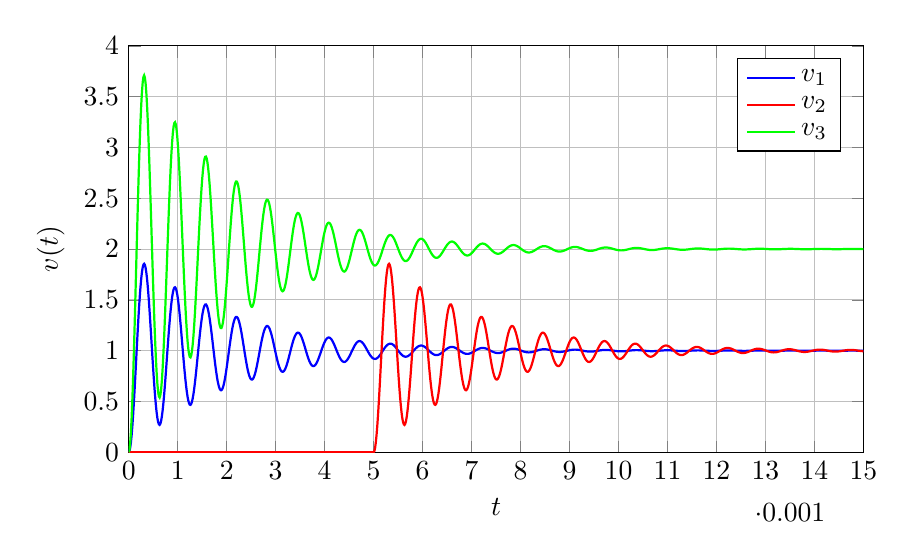
\begin{tikzpicture}
                        \begin{axis}[
                                width = 0.9\textwidth,
                                height = 0.9/1.618*\textwidth,
                                xlabel={$t$},
                                ylabel={$v(t)$},
                                xmin=0, xmax=0.015,
                                ymin=0, ymax=4,
                                xtick={0,0.001,...,0.015},
				xticklabel style={
				        /pgf/number format/fixed,
				        /pgf/number format/precision=3,
				},
				scaled x ticks={real:0.001},
                                ytick={0,0.5,...,4},
				samples=1000,
                                legend pos=north east,
                                ymajorgrids=true,
                                xmajorgrids=true,
                                every axis plot/.append style={thick, no marks},
                        ]    
                        \addplot[domain=0:0.015,thick,color=blue] {ceil(x)*( 1 - exp(-500*x)*( sin(10000*x*180/pi)/20 + cos(10000*x*180/pi)))};
                        \addplot[domain=0:0.015,thick,color=red ] {ceil(x-0.005)*( 1 - exp(-500*(x-0.005))*( sin(10000*(x-0.005)*180/pi)/20 + cos(10000*(x-0.005)*180/pi)))};
                        \addplot[domain=0:0.015,thick,color=green] {2*ceil(x)*( 1 - exp(-500*x)*( sin(10000*x*180/pi)/20 + cos(10000*x*180/pi)))};
			\legend{$v_1$,$v_2$,$v_3$}
                        \end{axis}
                \end{tikzpicture}
	\endpgfgraphicnamed
        \caption{Delayed response example of RLC circuit modelled.}
        \label{fig:delayed_example_rlc_ltiode}
\end{figure}
% >>>

\examplebar
\end{example} %>>>

%-------------------------------------------------
\section{Natural response of a LTI ODE} %<<<1

	The linearity and time invariance of Linear, Time Invariant Ordinary Differential Equations can be widely exploited to draw many properties; one of the many important aspects of LTI differential equations is that their response can be broken into two components: a ``natural'' component and a ``forced'' one. This fact plays a major role in the theory of Linear ODEs; particularly for this thesis, this fact is the main motivator for Phasor Theory as we want to show that, for a PLC, the homogeneous solution will always vanish in time, meaning that the particular solution will dominate over time.

\begin{theorem}[Homogeneous and particular solutions of LTI ODE]\label{theo:homogeneous_particular_ltiode} %<<<

	Consider the LTI ODE 

\begin{equation} \dot{\mathbf{x}} = \mathbf{A}\left[\mathbf{x}\right] + \mathbf{f}(t) . \label{eq:homo_theorem_homogeneous_ode_def_original}\end{equation}

	Let $\mathbf{X}_p$ be a known particular solution. Then the sum $\mathbf{x} = \mathbf{x_h} (t) + \mathbf{x_p}(t)$, where $\mathbf{x}_h$ a solution to the homogeneous (also called natural or non-forced) ODE

\begin{equation} \dot{\mathbf{x}}_\mathbf{h} = \mathbf{A}\left[\mathbf{x_h}\right] \label{eq:homo_theorem_homogeneous_ode_def},\end{equation}

	\noindent is also a solution to \eqref{eq:homo_theorem_homogeneous_ode_def_original}.

\end{theorem}
\noindent\textbf{Proof:} by definition the particular solution satisfies

\begin{equation} \dot{\mathbf{x}}_p = \mathbf{A}\left[\mathbf{x}_p\right] + \mathbf{f}(t) .\end{equation}

	Adopt $\mathbf{x}_h$ the solution to \eqref{eq:homo_theorem_homogeneous_ode_def} ; then

\begin{equation} \dot{\mathbf{x}}_p + \dot{\mathbf{x}}_h = \mathbf{A}\left[\mathbf{x}_p\right] + \mathbf{A}\left[\mathbf{x}_h\hphantom{x_P}\right] \mathbf{f}(t) .\end{equation}

	Using the linearity of the derivative and of $\mathbf{A}\left[\cdot\right]$,

\begin{equation} \dfrac{d}{dt} \left(\mathbf{x}_p + \mathbf{x}_h\right) = \mathbf{A}\left[\mathbf{x}_p + \mathbf{x}_h\right] + \mathbf{f}(t) .\end{equation}
\hfill$\blacksquare$
\vspace{5mm}
\hrule
\vspace{5mm} %>>>

	Another way of understanding theorem \ref{theo:homogeneous_particular_ltiode} is to write the excitation $\mathbf{f}$ can be written as $\mathbf{f} + \beta\mathbf{0}_n$, where $\mathbf{0}_n$ is the null vector of dimension $n$, for some scalar matrix $\beta\in\mathbb{C}^{\left(n\times m\right)}$; then

\begin{equation} \mathbf{G}\left[\mathbf{f} + \beta^\transpose\mathbf{0}\right] = \mathbf{G}\left[\mathbf{f}\right] + \beta^\transpose \mathbf{G}\left[\mathbf{0}\right] \end{equation}

	Therefore call $\mathbf{x}_h$ as 

\begin{equation} \mathbf{x}_h(t) = \mathbf{G}\left[\mathbf{0}\right]. \end{equation}

	\noindent that is, the response of the system with no forcing, or rather, ``natural'' response, and call

\begin{equation} \mathbf{x}_p(t) = \mathbf{G}\left[\mathbf{f}\right] \end{equation}

	\noindent as the excited or forced response. Then

\begin{equation} \mathbf{G}\left[\mathbf{f} + \beta^\transpose\mathbf{0}\right] = \mathbf{G}\left[\mathbf{f}\right] + \beta^\transpose\mathbf{G}\left[\mathbf{0}\right] = \mathbf{x}_p +\beta^\transpose\mathbf{x}_h , \end{equation}

	The beauty of this fact is that the general solution of a particular LTI ODE can be found through only two functions: a particular solution and the homogeneous solution. If these two are found, then for any solution $\mathbf{x}$ of this ODE there is a $\beta$ such that

\begin{equation} \mathbf{x}(t) = \mathbf{x}_p(t) + \beta^\transpose\mathbf{x}_h(t) \end{equation}

	\noindent and, because of the differential nature of the system, $\beta$ is only determined by the initial conditions:

\begin{equation} \mathbf{x}(0) = \mathbf{x}_p(0) + \beta^\transpose\mathbf{x}_h(0) \Leftrightarrow \left(\mathbf{x}(0) - \mathbf{x}_p(0)\right) = \beta^\transpose\mathbf{x}_h(0) \end{equation}

	The benefit of separating the response of an LTI ODE into natural and forced behaviors is that, as equation \eqref{eq:homo_theorem_homogeneous_ode_def} shows, the natural homogeneous response does not depend on the forcing because, by definition, it is calculated when the system is not forced. For this reason, $\mathbf{x}_h$ is also called the system \textit{natural response}, and $\mathbf{x}_p$ the system \textit{forced response}.

\begin{example}\label{example:rlc_circuit_natural_example} % EXAMPLE OF LTI ODE CIRCUIT MODELLING <<<
	Consider again the RLC circuit of figure \ref{fig:ltiode_modelling_example_circuit} in example \ref{example:rlc_circuit_lti_ode_example} where an RLC circuit is shown and which modelling is given by

\begin{equation} LC\dfrac{d^2v(t)}{dt^2} + \dfrac{L}{R}\dfrac{dv(t)}{dt} + v(t) - u(t) = 0 \end{equation}

	With $L = 10$mH, $C = 1\mu$F and $R = 1$k$\Omega$. Suppose that the system is excited by a cosine:

\begin{equation} LC\dfrac{d^2v(t)}{dt^2} + \dfrac{L}{R}\dfrac{dv(t)}{dt} + v(t) - M\cos\left(\omega t\right) = 0 \label{eq:example2_original_ode}\end{equation}

	\noindent then, solving the homogeneous ODE yields the natural response

\begin{equation} LC\dfrac{d^2v_h(t)}{dt^2} + \dfrac{L}{R}\dfrac{dv_h(t)}{dt} + v_h(t) = 0 \end{equation}

	\noindent by inspection it can be shown that $e^{kt}$ is a solution where

\begin{equation} k = \dfrac{-\dfrac{L}{R} \pm \sqrt{\left(\dfrac{L}{R}\right)^2 - 4LC} }{2LC} = -\dfrac{1}{2RC} \pm \sqrt{\left(\dfrac{1}{2RC}\right)^2 - \dfrac{1}{LC}} .\end{equation}

	For a numerical example, consider $L = 10$mH, $C = 1\mu$F and $R = 1$k$\Omega$, $M = 1V$ and $\omega = 500$ rad.s$^{-1}$. These values yield a pair of conjugate complex solutions. Because $v_h$ is real, these solutions amount to

\begin{equation} x_h(t) = c_he^{-k_R t} \cos\left(k_I t\right) \label{example:rlc_circuit_natural_example_homogeneous} \end{equation}

	\noindent where $c_h$ is a constant that can be drawn from initial conditions and

\begin{equation} k_R = \dfrac{1}{2RC},\ k_I = \pm j\ \sqrt{\dfrac{1}{LC} - \left(\dfrac{1}{2RC}\right)^2} .\end{equation}

	For the particular solution, suppose $v_p = A\sin\left(\omega t\right) + B\cos\left(\omega t\right)$, yielding

\begin{gather} -LC\omega^2\left[A\sin\left(\omega t\right) + B\cos\left(\omega t\right) \right] + \nonumber\\[5mm]\hspace{1cm} \dfrac{L}{R}\omega \left[A\cos\left(\omega t\right) - B\sin\left(\omega t\right) \right] + \nonumber\\[5mm]\hspace{3cm} A\sin\left(\omega t\right) + B\cos\left(\omega t\right) - M\cos\left(\omega t\right) = 0 \end{gather}

	Grouping the terms,

\begin{equation} \sin\left(\omega t\right) \left( -LC\omega^2 A - \dfrac{L\omega}{R}B + A\right) + \cos\left(\omega t\right)\left(-LC\omega^2 B + \dfrac{L\omega}{R}A + B - M\right) = 0 \end{equation}

	Because sine and cosine are orthogonal, this can only be possible if

\begin{equation}\left\{\begin{array}{l} -LC\omega^2 A - \dfrac{L\omega}{R}B + A = 0 \\[5mm] -LC\omega^2 B + \dfrac{L\omega}{R}A + B - M = 0 \end{array}\right. \Leftrightarrow \left\{\begin{array}{l} \left(1 -LC\omega^2\right) A - \dfrac{L\omega}{R}B = 0 \\[5mm] \left(1 - LC\omega^2 \right) B + \dfrac{L\omega}{R}A - M = 0 \end{array}\right. \end{equation}
	
	From the first equation,

\begin{equation}  A = \dfrac{L\omega}{R\left(1 -LC\omega^2\right)}B  \end{equation}

	\noindent and substituting on the second,

\begin{gather}
	\left(1 - LC\omega^2 \right) B + \dfrac{L\omega}{R}\dfrac{L\omega}{R\left(1 -LC\omega^2\right)}B - M = 0 \nonumber\\[5mm]
	\left[\left(1 - LC\omega^2 \right)^2 + \left(\dfrac{L\omega}{R}\right)^2 \right] B - M\left(1 - LC\omega^2 \right) = 0 \nonumber\\[5mm]
	B = M\xfrac{2mm}{5mm}{\left(1 - LC\omega^2 \right)}{\left[\left(1 - LC\omega^2 \right)^2 + \left(\dfrac{L\omega}{R}\right)^2 \right]} \Leftrightarrow A = M\xfrac{2mm}{5mm}{\left( \dfrac{\omega L}{R} \right)}{\left[\left(1 - LC\omega^2 \right)^2 + \left(\dfrac{L\omega}{R}\right)^2 \right]}
\end{gather}

	Therefore let $\sqrt{A^2 + B^2} = M$ and $\phi$ such that

\begin{equation} \tan\left(\phi\right) = \dfrac{A}{B} = \xfrac{3mm}{2mm}{\dfrac{\omega L}{R}}{ 1 - LC\omega^2} \end{equation}

	\noindent then the general solution of the particular solution is

\begin{equation} x_p = c_p\cos\left(\omega t + \phi\right) \label{example:rlc_circuit_natural_example_particular} \end{equation}

	\noindent with $c_p$ another constant that can be obtained from initial conditions. Therefore, a solution to the excited ODE \eqref{eq:example2_original_ode} is a the sum of \eqref{example:rlc_circuit_natural_example_homogeneous} and \eqref{example:rlc_circuit_natural_example_particular}:

\begin{equation} x(t) = c_he^{-k_R t} \cos\left(k_I t\right) + c_p\cos\left(\omega t + \phi\right) \label{eq:example2_original_ode_homo}\end{equation}

	\noindent where the $c_p$ and $c_h$ are constants respective to initial conditions. At this point of the text, this solution is still \textit{a solution}, but it will be shown later that it is actually the \textit{general solution}, that is, any solution to the original forced ODE \eqref{eq:example2_original_ode} is obtained by varying $c_p$ and $c_h$ on \eqref{eq:example2_original_ode_homo}. For a specific example, supposing $x(0) = M$ and $x'(0) = 0$,

\begin{equation} \left\{\begin{array}{l} M = c_h + c_p\cos\left(\phi\right) \\[5mm] 0 = -c_hk_R - c_p\omega\sin\left(\phi\right) \end{array}\right. \end{equation}

	Multiply the first equation by $k_R$ and sum to the second:

\begin{equation} c_p = \dfrac{Mk_R}{k_R\cos\left(\phi\right) - \omega\sin\left(\phi\right)} \end{equation}

	\noindent therefore

\begin{equation} c_h = M - \cos\left(\phi\right)\left[\dfrac{Mk_R}{k_R\cos\left(\phi\right) - \omega\sin\left(\phi\right)}\right] = -\dfrac{M\omega \sin\left(\phi\right)}{k_R\cos\left(\phi\right) - \omega\sin\left(\phi\right)}\end{equation}

\examplebar
\end{example} %>>>

	Because the natural response of an LTIODE is independent of the excitation, one might ask what is its shape and the characteristics; the first step in the discussion is to show that the general solution to the homogeneous part $\mathbf{x}_h$ is easily achievable when a certain equivalent matrix $\mathbf{A}$ is diagonalizable. If such is not the case, then a more refined discussion is made under the framework of linear algebra and linear differential equations to deal with the case that $\mathbf{A}$ is not diagonalizable, also called defective.

	The ultimate objective of this subsection is to show that it is possible to define a complex matrix exponential function such that the general solution to the natural part can be written as $\mathbf{x} = e^{\mathbf{A}t}\mathbf{x}_0$; this is motivated by the fact that the general solution to a one-dimensional ODE $\dot{x}(t) = ax(t)$ is $x(t) = e^{at}x_0$. Then, it is shown that if this equivalent matrix has certain properties, namely that its eigenvalues all have negative real part, then the natural part of the general solution vanishes in time in a strong exponential sense, leaving only the particular solution as time grows. In Classical and Dynamic Phasor Theory, this is of utmost importance because the particular solution $\mathbf{x_p}$ is somehwat simple to find, and because $\mathbf{x_h}$ vanishes as time grows, the solution $\mathbf{x_p}$ dominates over time. In other words, phasors are a particularization of the solution of the LTIODE when the transient behavior is disconsidered and the steady-state dominates over time.

	In order to achieve this, we must first define what a diagonalizable operator is, which needs the ideas of fields, matrices and bases.

%-------------------------------------------------
\section{Bases, matrices and operations}\label{sec:bases_matrices_operations} %<<<1

	Let $\mathbf{U} = \left(\mathbf{u}_1,\mathbf{u}_2,...,\mathbf{u}_k\right)$ be a sequence of $k$ arbitrary vectors. Adopt a collection of scalars $\left(z_1,z_2,...,z_k\right)$ and the expression

\begin{equation} \mathbf{m} = z_1\mathbf{u}_1 + z_2\mathbf{u}_2 + \cdots + z_k\mathbf{u}_k \end{equation}

	\noindent is called a \textbf{linear combination} of the $\mathbf{u}_i$. Further, the \textbf{span} of the set is defined as the collection of all vectors that can be written as a linear combination of the $\mathbf{u}_i$:

\begin{equation} \mathspan\left(\mathbf{U}\right) = \left\{\sum\limits_{i=1}^k z_i\mathbf{u}_i : z_i\text{ is a scalar}\right\}\end{equation}
	
	\noindent and if a certain set $\mathbf{W}$ is the span of some set $\mathbf{U}$ we say that $\mathbf{U}$ \textbf{generates} $\mathbf{W}$, or is a \textbf{generating set} of $\mathbf{W}$. In that case, a particular vector $\mathbf{x}\in\mathbf{W}$ is expressed as a linear combination of the vectors in this generating set, that is,

\begin{equation} \mathbf{x} = \sum_{i=1}^k x_i\mathbf{u}_i\end{equation}

	\noindent where the $x_k$ are scalars in the field $F$ that the vector space is defined over. Naturally, if the generating set changes, then the $x_i$ also change; in this case, $\mathbf{x}$ can be represeted by the tuple $\left(x_i\right)_{i=1}^k$ with respect to the specific generating set $\mathbf{U}$. We define this as a columnar arrangement known as coordinates:

\begin{equation} \left[\mathbf{x}\right]_\mathbf{U} = \sum\limits_{i=1}^k x_i \mathbf{u}_i \vcentcolon = \left[\begin{array}{c} x_1 \\[3mm] x_2 \\[3mm] \vdots \\[3mm] x_k \end{array}\right]_{\mathbf{U}}\end{equation}

	\noindent meaning $\left[\mathbf{x}\right]_{\mathbf{U}} = \left[x_1,x_2,\cdots,x_k\right]^\transpose$ is the representation of $\mathbf{x}$ on (or against) $\mathbf{U}$. It must be noted that because the coordinates $x_i$ are unique, the relationship $\left(x_1,x_2,\cdots,x_n\right) \leftrightarrow \mathbf{x}$ is bijective and uniquely defined, therefore an \textbf{isomorphism}.

	The space of $n$ coordinates in $F$ is denoted $F^n$, an allusion to the fact that formally this space is defined as a cartesian product $F\times F\times ... \times F$, $n$ times. In some cases it is interesting to display this arrangement in a horizontal matter, so we define the \textbf{transposition} operation, denoted with a superscript $\transpose$, that transforms a columnar arrangement into a horizontal one and vice-versa:

\begin{equation} \left[\begin{array}{c} x_1 \\[3mm] x_2 \\[3mm] \vdots \\[3mm] x_k \end{array}\right]^\transpose = \left[x_1,x_2,\cdots,x_k\right] \text{, and } \left[y_1,y_2,\cdots,y_k\right]^\transpose =  \left[\begin{array}{c} y_1 \\[3mm] y_2 \\[3mm] \vdots \\[3mm] y_k \end{array}\right] .\end{equation}

	Hereforth, we assume that that the domain of $\mathbf{A}$ can be defined over the complex numbers, that is, $F = \mathbb{C}$, meaning every vector in that domain can be represented as a set of $n$ complex coordinates. Naturally the question becomes what is the minimum or ``smallest'' generating set that a certain space can have. A \textbf{basis} (plural \textbf{bases}) of a space is a collection $\mathbf{V} = \left(\mathbf{v}_1,\mathbf{v}_2,...,\mathbf{v}_k\right)$ of \textbf{linearly independent} vectors, that is, a set such that no single component can be written as a linear combination of the others, and $\mathbf{V}$ generates that particular set. Linear independence means that for a collection of scalars $z_k$, the linear combination of the $\mathbf{v}_k$ is anihilated if and only if the scalars are null:

\begin{equation} \mathbf{0} = z_1 \mathbf{v}_1 + z_2\mathbf{v}_2 + ... + z_k \mathbf{v}_n \Leftrightarrow z_1 = z_2 = ... = z_k = 0.\end{equation}

	It follows that any vector $\mathbf{x}$ can be written as a unique linear combination of the vectors in $\mathbf{V}$: write

\begin{equation} \mathbf{x} = \beta_1 \mathbf{v}_1 + \beta_2\mathbf{v}_2 + ... + \beta_k \mathbf{v}_k \end{equation}

	\noindent where the $\beta_k$ are the \textbf{coordinates of} $\mathbf{x}$ in the basis $\mathbf{V}$. Suppose $\mathbf{x}$ has a second representation of coordinates $\gamma_k$:

\begin{equation} \mathbf{x} = \gamma_1 \mathbf{v}_1 + \gamma_2\mathbf{v}_2 + ... + \gamma_k \mathbf{v}_k \end{equation}

	\noindent subtracting both equations yields

\begin{equation} \mathbf{0} = \left(\gamma_1 - \beta_1\right) \mathbf{v}_1 + \left(\gamma_2 - \beta_2\right)\mathbf{v}_2 + ... + \left(\gamma_k - \beta_k\right) \mathbf{v}_k \end{equation}

	\noindent which can only be possible if $\beta_i = \gamma_i$, for all $i$, due to the linear independency of the vectors in the basis.

	A vector space $V$ has dimension $n$, denoted $\dim\left(V\right)$, if such is the smallest number of vectors a basis needs to have in that space, or equivalently, the least number of vectors a generating set has to have to be a basis of that space. It is a direct consequence of their definitions, and a paramount property of bases, that their span is the whole of the vector space they are immersed in; saying a vector space has dimension $n$ means exactly $n$ linearly independent vectors are needed to form a basis for it. It is obvious that $\mathbb{C}^n$ has dimension $n$.

	Naturally one asks what is the dimension of the space $\left[\mathbb{R}\to\mathbb{C}\right]$. Unfortunately such a basis does not exist; there does not exists a finite (or infinite, for this matter) set of elements that generates the entire space. There do exist, however, bases for specific subspaces. (Famously, the space of square-Lebesgue-integrable functions $L^2$ has an inner product that induces a basis which itself induces famous transforms as its inner product like Fourier and Laplace, which will be used in the later chapters of this text). For example, if we restrict the space of functions to those that solve the linear ODE being studied, theorem \ref{theo:ode_sol_space_dim} shows that the restricted space has dimension of the order of the ODE.

\begin{theorem}[Dimension of the space of solutions of an ODE]\label{theo:ode_sol_space_dim} %<<<
	The space of solutions of the linear ODE $\dot{\mathbf{x}} = \mathbf{A}\left[\mathbf{x}\right]$, in $\left[\mathbb{R}\to\mathbb{C}^n\right]$ has dimension $n$.
\end{theorem}
\noindent\textbf{Proof.} Let $\mathbf{V} = \left(\mathbf{v}_k\right)_{k=1}^n$ a set of $n$ linearly independent vectors in this space. This means that for any time $t$,

\begin{equation} \sum_{k=1}^n \alpha_k \mathbf{v}_k(t) = \mathbf{0}(t)\Leftrightarrow \alpha_1 = \alpha_2 = ... = \alpha_n .\end{equation}

	\noindent where $\mathbf{0}(t)$ here represents the null function, that is, $\mathbf{0}(t) = \left[0(t),0(t),0(t),...,0(t)\right]^\transpose$ for all times. Consider a vector $\mathbf{u}$ in the span of $\mathbf{V}$

\begin{equation} \mathbf{u} = \sum_{k=1}^n \alpha_k \mathbf{v}_k.\end{equation}

	Then

\begin{equation} \dfrac{d\mathbf{u}}{dt} = \dfrac{d}{dt}\left(\ \sum_{k=1}^n \alpha_k \mathbf{v}_k\right) \end{equation}

	\noindent and using that the differential transform is linear,

\begin{equation} \dfrac{d}{dt}\left(\ \sum_{k=1}^n \alpha_k \mathbf{v}_k\right) = \sum_{k=1}^n \alpha_k \dot{\mathbf{v}}_k \end{equation}

	\noindent but since each $\mathbf{v}_k$ is a solution of the ODE,

\begin{equation} \sum_{k=1}^n \alpha_k \dot{\mathbf{v}}_k = \sum_{k=1}^n \alpha_k \mathbf{A}\left[\mathbf{v}_k\right]   \end{equation}

	\noindent and using the linearity of $\mathbf{A}\left[\cdot\right]$,

\begin{equation} \sum_{k=1}^n \alpha_k \mathbf{A}\left[\mathbf{v}_k\right] = \mathbf{A}\left[\sum_{k=1}^n \alpha_k \mathbf{v}_k\right] = \mathbf{A}\left[\mathbf{u}\right] \end{equation}

	\noindent meaning $\mathbf{u}$ is a solution to $\dot{\mathbf{u}} = \mathbf{A}\left[\mathbf{u}\right]$, that is, $\mathbf{V}$ generates some solutions of the ODE. We now prove it actually generates all solutions. Suppose the contrary, that it does not generate all of them and that there exists a $\mathbf{v}_{(n+1)}$ that is also a solution of the ODE but is linearly independent of all the $\mathbf{v}_k$, meaning

\begin{equation} \sum_{k=1}^{(n+1)} \alpha_k \mathbf{v}_k = \mathbf{0}(t)\Leftrightarrow \alpha_k = 0,\ k\in\mathbb{N}_{(n+1)}^* .\end{equation}

	We now ``freeze'' this equation in time: for each time $t = a$,

\begin{equation} \sum_{k=1}^{(n+1)} \alpha_k \mathbf{v}_k(a) = \mathbf{0},\ k\in\mathbb{N}_{(n+1)}^* . \end{equation}

	\noindent where $\mathbf{0}$ is the null complex vector. This cannot be true because the $\mathbb{C}^n$ has dimension $n$; yet this equation dictates that there exist $n+1$ linearly independent vectors in $\mathbb{C}^n$. Therefore, at all times $t$ there must be some linear combination among the complex vectors $\mathbf{v}_k(t=a)$, which then means there must be a linear combination among the $\mathbf{v}_k$, contradicting the supposition.
\hfill$\blacksquare$
\vspace{5mm}
\hrule
\vspace{5mm} %>>>

	Therefore, notwithstanding the fact that $\left[\mathbb{R}\to\mathbb{C}^n\right]$ does not have a basis (because there needs to be an uncountable infinite number of vectors), the set of solutions of the ODE $\dot{\mathbf{x}} = \mathbf{A}\left[\mathbf{x}\right]$ defined by $\mathbf{A}$ in that space does have dimension $n$. Due to this fact, in the specific case of this differential equation we define $\Dom\left(\mathbf{A}\right)$ as the space of solutions of that ODE defined by $\mathbf{A}$, as opposed to its proper domain.

	It will be shown that bases are somewhat equivalent in the sense a vector representation in a particular base can be changed to a representation on another base and that, despite this process being possible, linear functionals have certain properties that are unwaivering to a base change. It is however natural to assume a certain fixed or natural basis can be adopted to establish common grounds of representation; for instance, adopting the canonical basis $\mathbf{I}_n$ for $\mathbb{C}^n$ composed of the vectors $\mathbf{e}_k$, $1\leq k \leq n$, which contain a unitary element on the k-th positions and zero everywhere else:

\begin{equation} \mathbf{I}_n = \left(\mathbf{e}_1,\mathbf{e}_2,\mathbf{e}_3,...,\mathbf{e}_n\right) = \left( \left[\begin{array}{c} 1 \\[3mm] 0 \\[3mm] 0 \\[3mm] \vdots \\[3mm] 0 \end{array}\right], \left[\begin{array}{c} 0 \\[3mm] 1 \\[3mm] 0 \\[3mm] \vdots \\[3mm] 0 \end{array}\right], \left[\begin{array}{c} 0 \\[3mm] 0 \\[3mm] 1 \\[3mm] \vdots \\[3mm] 0 \end{array}\right], ..., \left[\begin{array}{c} 0 \\[3mm] 0 \\[3mm] 0 \\[3mm] \vdots \\[3mm] 1 \end{array}\right] \right) \label{eq:canonical_basis_complex}\end{equation}

	\noindent and let us define the canonical  basis of the solutions of the ODE as $\left(\mathbf{v}_1,\mathbf{v}_2,\mathbf{v}_3,...,\mathbf{v}_n\right)$ where each $\mathbf{v}_k$ is the canonical vector $\mathbf{e}_k$ at an initial time $t_0$ that is, $\mathbf{v}_k$ is defined as the vector function that satisfies

\begin{equation} \left\{\begin{array}{l} \dot{\mathbf{v}}_k = \mathbf{A}\left[\mathbf{v}_k\right] \\[3mm] \mathbf{v}_k\left(t_0\right) = \mathbf{e}_k \end{array}\right. .\end{equation}

	One asks whether the $\mathbf{v}_k$ exist and are unique, and the answer is yes: this is easily provable using the Banach-Cacciopoli Fixed Point Theorem. For now we do not prove this fact since we are more interested in the qualities of the $\mathbf{v}_k$ as a basis. Now establish the bijection

\begin{equation} \phi: \left\{\begin{array}{rcl} \Dom\left(\mathbf{A}\right) &\to& \mathbb{C}^n \\[3mm] \mathbf{v}_k &\mapsto& \mathbf{e}_k \end{array}\right. \end{equation}

	\noindent (the notation $\Dom\left(\mathbf{A}\right)$ here is not understood as the proper domain $\left[\mathbb{R}\to\mathbb{C}^n\right]$ but the restriction of this space to the subspace of functions that satisfy the ODE defined by $\mathbf{A}\left[\cdot\right]$). We want to use this bijection to show that any vector in $\Dom\left(\mathbf{A}\right)$ admits a representation in $\mathbb{C}^n$ using the chosen basis $\mathbf{V}$. First we note that this bijection is a morphism between $\Dom\left(\mathbf{A}\right)$ and $\mathbb{C}^n$, that is, it preserves the algebraic structures and operations of sum and multiplication by scalar; particularly, any linear combination in $\Dom\left(\mathbf{A}\right)$ remains in $\mathbb{C}^n$, that is, for any $\mathbf{v},\mathbf{w}\in\Dom\left(\mathbf{A}\right)$ and any $\alpha\in\mathbb{C}$,

\begin{equation} \phi\left(\mathbf{v} + \alpha\mathbf{w}\right) = \phi\left(\mathbf{v}\right) + \alpha\phi\left(\mathbf{w}\right) .\end{equation}

	Further, we can show that because $\phi$ maps each $\mathbf{v}_k$ specifically to the $k$-th vector $\mathbf{e}_k$ of the canonical basis of $\mathbb{C}^n$, then $\phi$ is unique. This fact allows us to represent any $\mathbf{x}\in\Dom\left(\mathbf{A}\right)$ as coordinates on the chosen basis $\mathbf{V}$,

\begin{equation} \left[\mathbf{x}\right]_{\mathbf{V}} = \sum\limits_{k=1}^n x_k \mathbf{v}_k .\end{equation}

	\noindent then we can establish a representation of $\mathbf{x}$ into the $\mathbb{C}^n$ by using $\phi$ and its linearity:

\begin{equation} \phi\left(\left[\mathbf{x}\right]_{\mathbf{V}}\right) = \phi\left(\sum\limits_{k=1}^n x_k \mathbf{v}_k\right) = \sum\limits_{k=1}^n x_k \phi\left(\mathbf{v}_k\right) = \sum\limits_{k=1}^n x_k \mathbf{e}_k .\end{equation}

	Therefore $\phi\left(\left[\mathbf{x}\right]_{\mathbf{V}}\right)$ has a set of coordinates in $\mathbb{C}^n$ identical to the coordinates of $\mathbf{x}$ in $\mathbf{V}$ but using the canonical basis $\mathbf{I}_n$ for $\mathbb{C}^n$. Thus we can adopt the representation of $\mathbf{x}$ with respect to the canonical basis of $\mathbb{C}^n$ as

\begin{equation} \left[\mathbf{x}\right]_{\mathbf{I}_n} = \phi\left(\left[\mathbf{x}\right]_{\mathbf{V}}\right) = \sum\limits_{k=1}^n x_k \mathbf{e}_k .\end{equation}

	In other words, $\mathbf{x}$ is represented as a point in $\mathbb{C}^n$, meaning that an analysis on $\Dom\left(\mathbf{A}\right)$ is equivalent to an analysis on $\mathbb{C}^n$. Further, the basis $\mathbf{V}$ also induces a canonical matrix form for the linear map $\mathbf{A}\left[\cdot\right]$, denoted $\left[\mathbf{A}\right]_{\mathbf{I}_n}$: exploring the linearity of $\mathbf{A}\left[\cdot\right]$ one yields

\begin{equation}
	\mathbf{A}\left[\mathbf{x}\right]_{\mathbf{V}} = \mathbf{A}\left[\begin{array}{c} x_1 \\[3mm] x_2 \\[3mm] \vdots \\[3mm] x_n\end{array} \right]_\mathbf{V} = \mathbf{A}\left[\sum\limits_{k=1}^n x_k\mathbf{v}_k \right] = \sum_{k=1}^n x_k\mathbf{A}\left[\mathbf{v}_k\right] \label{eq:Aappliedtox} .% =  \left[\begin{array}{c} a_{11}x_1(t) + a_{12}x_2(t) + ... + a_{1n}x_n(t) \\[3mm] a_{21}x_1(t) + a_{22}x_2(t) + ... + a_{2n}x_n(t) \\[3mm] \vdots \\[3mm]  a_{n1}x_1(t) + a_{n2}x_2(t) + ... + a_{nn}x_n(t) \end{array}\right]
\end{equation}

	Therefore, operating a vector $\mathbf{x}$ through $\mathbf{A}\left[\mathbf{x}\right]$ can be (instead of direct calculation) found simply if one knows the coordinates of $\mathbf{x}$ with respect to $\mathbf{V}$ (which are the same as with repect to $\mathbf{I}_n$) and how $\mathbf{A}\left[\cdot\right]$ transforms each of the canonical vectors $\mathbf{v}_k$. But seen as each $\mathbf{A}\left[\mathbf{v}_k\right]$ is a vector itself, it has coordinates on $\mathbf{V}$:

\begin{equation} \mathbf{A}\left[\mathbf{v}_k\right] = \left[\begin{array}{c} a_{1k} \\[3mm] a_{2k} \\[3mm] \vdots \\[3mm] a_{nk} \end{array}\right]_\mathbf{V}\end{equation}

	\noindent and because $\phi$ is bijective and unique, we can represent $\mathbf{A}\left[\cdot\right]$ uniquely by the $\mathbf{A}\left[\mathbf{v}_k\right]$; therefore, we can arrange the $\mathbf{A}\left[\mathbf{v}_k\right]$ into a tabular arrangement that we will call a \textbf{matrix}, by using these vectors as the columns. This matrix is denoted $\mathbf{A}$:

\begin{equation} \mathbf{A} = \left[\raisebox{15mm}{} \begin{array}{cccc} \left[\begin{array}{c} \vdots \\[3mm] \mathbf{A}\left[\mathbf{v}_1\right] \\[3mm] \vdots \end{array}\right] & \left[\begin{array}{c} \vdots \\[3mm] \mathbf{A}\left[\mathbf{v}_2\right] \\[3mm] \vdots \end{array}\right] & ... & \left[\begin{array}{c} \vdots \\[3mm] \mathbf{A}\left[\mathbf{v}_n\right] \\[3mm] \vdots \end{array}\right]\end{array}\right] = \left[\begin{array}{cccc} a_{11} & a_{12} & ... & a_{1n} \\[3mm] a_{21} & a_{22} & ... & a_{2n} \\[3mm] \vdots & \vdots & \ddots & \vdots \\[3mm]  a_{n1} & a_{n2} & ... & a_{nn} \end{array}\right]  . \label{eq:tabular_arrangement}\end{equation}

	\noindent or we can see a matrix as an arrangement of $n$ vectors of dimension $n$ as its rows:

\begin{equation} \mathbf{A} = \left[\begin{array}{c} \left[\cdots\ \mathbf{r}_1\ \cdots \right] \\[5mm] \left[\cdots\ \mathbf{r}_2\  \cdots \right] \\[5mm]  \vdots  \\[5mm] \left[\cdots\ \mathbf{r}_n\ \cdots \right] \end{array}\right] \end{equation}

	\noindent such that rows and columns can be ``rotated'' through a version of the \textbf{transposition} operation for matrices, that is, the transpose of $\mathbf{A}$, denoted $\mathbf{A}^\transpose$, is the matrix which rows and the columns of $\mathbf{A}$ and vice-versa:

\begin{equation} \mathbf{A}^\transpose = \left[\raisebox{15mm}{} \begin{array}{cccc} \left[\begin{array}{c} \vdots \\[3mm] \mathbf{r}_1 \\[3mm] \vdots \end{array}\right] & \left[\begin{array}{c} \vdots \\[3mm] \mathbf{r}_2 \\[3mm] \vdots \end{array}\right] & ... & \left[\begin{array}{c} \vdots \\[3mm] \mathbf{r}_n \\[3mm] \vdots \end{array}\right]\end{array}\right] = \left[\begin{array}{c} \left[\cdots\ \mathbf{c}_1\ \cdots \right] \\[5mm] \left[\cdots\ \mathbf{c}_2\  \cdots \right] \\[5mm]  \vdots  \\[5mm] \left[\cdots\ \mathbf{c}_n\ \cdots \right] \end{array}\right] .\end{equation}

	\noindent and it can be shown that the relationship between matrix and functional is bijective, meaning that the matrix $\mathbf{A}$ is a particular matrix representation of the linear operator $\mathbf{A}\left[\cdot\right]$ when the canonical basis is adopted. The underlying implication is that the matrix $\mathbf{A}$, called the \textbf{canonical representation} of the linear functional $\mathbf{A}\left[\cdot\right]$, is such that they can be interpreted as the same entity in some sense.

	Equation \eqref{eq:Aappliedtox} then defines that the linear transform $\mathbf{A}\left[\cdot\right]$ applied to a particular vector $\mathbf{x}$, becomes a linear combination of the column vectors of the canonical matrix representation $\mathbf{A}$ where the coefficients of the combination are the coordinates of $\mathbf{x}$. Because of this, we can define a matrix-by-vector multiplication as the linear combination of the column vectors.

\begin{definition}[Matrix-by-vector multiplication]\label{def:matrixbyvector} Let $\mathbf{A}\in\mathbb{C}^{(n\times n)}$, $\mathbf{c}_k,\ k\in\mathbb{N}^*_n$ its column vectors, and $\mathbf{x} = \left[x_1,x_2,...,x_n\right]^\transpose\in\mathbb{C}^n$. Then the multiplication $\mathbf{Ax}$ is defined as

\begin{equation} \mathbf{Ax} = \sum_{k=1}^n x_k\mathbf{c}_k \end{equation}
\end{definition}

	And the idea is that defining such multiplication this way makes the application $\mathbf{A}\left[\mathbf{x}\right]$ a simple multiplication in $\mathbb{C}^n$, while retaining algebraic structions and retaining the bijection $\phi$ between $\Dom\left(\mathbf{A}\right)$ and $\mathbb{C}^n$, as denoted in theorem \ref{theo:bij_v_cnmaintained}, easily proven by inspection.

\begin{theorem}\label{theo:bij_v_cnmaintained} Let $\mathbf{A}\left[\cdot\right]$ some linear map with, $\mathbf{x}\in\Dom\left(\mathbf{A}\right)$ and $\mathbf{V}$ the canonical basis of the domain. Then the coordinates of the vector $\mathbf{A}\left[\mathbf{x}\right]$ in $\mathbf{V}$ are the same coordinates than the multiplication $\left[\mathbf{A}\right]_{\mathbf{I}_n} \left[\mathbf{x}\right]_{\mathbf{I}_n}$, that is,

\begin{equation} \left[\raisebox{1mm}[2mm][2mm]{} \mathbf{A}\left[\mathbf{x}\right]\right]_\mathbf{V} = \left[\mathbf{A}\right]_{\mathbf{I}_n} \left[\mathbf{x}\right]_{\mathbf{I}_n}\end{equation}
\end{theorem}
\hrule
\vspace{3mm}

	Using definition \ref{def:matrixbyvector} we can simplify the application $\mathbf{A}\left[\mathbf{x}\right]$ to a multiplication $\mathbf{Ax}$. The linearity property of this multiplication is immediately provable. If we repeat this same line of thought for horizontal vectors, we achieve a similar result in horizontal form, the idea being that instead of producing column vectors we can produce row vectors by transposing the multiplication.

\begin{definition}[Vector-by-matrix multiplication]\label{def:vectorbymatrix} Let $\mathbf{A}\in\mathbb{C}^{(n\times n)}$, $\mathbf{r}_k,\ k\in\mathbb{N}^*_n$ its row vectors, and $\mathbf{x} = \left[x_1,x_2,...,x_n\right]\in\mathbb{C}^n$. Then the multiplication $\mathbf{xA}$ is defined as

\begin{equation} \mathbf{xA} = \sum_{k=1}^n x_k\mathbf{r}_k \end{equation}
\end{definition}
\begin{theorem}\label{theo:vector_trasnp} Let $\mathbf{A}\in\mathbb{C}^{(n\times n)}$ and $\mathbf{x} = \left[x_1,x_2,...,x_n\right]^\transpose\in\mathbb{C}^n$. Then $\left(\mathbf{Ax}\right)^\transpose = \mathbf{x}^\transpose\mathbf{A}^\transpose$.
\end{theorem}
\hrule
\vspace{3mm}

	It is clear that in order for the matrix-by-vector operation to be feasible, the vector $\mathbf{x}$ has to have as many elements as the matrix $\mathbf{A}$ has rows, whereas for vector-by-matrix, $\mathbf{x}$ has to have as many elements as $\mathbf{A}$ has columns. Thence, the ODE \eqref{eq:matrix_lti_ode_eq_def} can be written as

\begin{equation} \dfrac{d}{dt} \left[\mathbf{x} \right]_{\mathbf{I}_n} = \left[\mathbf{A}\right]_{\mathbf{I}_n}\left[\mathbf{x}\right]_{\mathbf{I}_n} + \left[\mathbf{f}\right]_{\mathbf{I}_n} . \label{eq:equivalent_lti_ode_operator} \end{equation}

	\noindent where it must be understood that $\left[\mathbf{x} \right]_{\mathbf{I}_n}$ is a time-varying quantity. In order to simplify notation, and seen as due to the bijection $\phi$ the representation in $\mathbf{V}$ and in $\mathbf{I}_n$ are the same, then hereforth we just write


\begin{equation} \dot{\mathbf{x}} = \mathbf{Ax} + \mathbf{f} . \label{eq:equivalent_lti_ode_operator} \end{equation}

	For completude, we can also define a matrix-by-matrix multiplication as an operation induced by the matrix-by-vector multiplication.

\begin{definition}[Matrix-by-matrix multiplication]\label{def:matrixbymatrix}  Let $\mathbf{A,B}\in\mathbb{C}^{(n\times n)}$, $\mathbf{b}_k,\ k\in\mathbb{N}^*_n$ the column vectors of $\mathbf{B}$. Then the multiplication $\mathbf{AB}$ is defined as the matrix which columns are the multiplications of $\mathbf{A}$ by the columns of $\mathbf{B}$:

\begin{equation} \mathbf{AB} = \left[\raisebox{15mm}{} \begin{array}{cccc} \left[\begin{array}{c} \vdots \\[3mm] \mathbf{A}\mathbf{b}_1 \\[3mm] \vdots \end{array}\right] & \left[\begin{array}{c} \vdots \\[3mm] \mathbf{A}\mathbf{b}_2 \\[3mm] \vdots \end{array}\right] & ... & \left[\begin{array}{c} \vdots \\[3mm] \mathbf{A}\mathbf{b}_n \\[3mm] \vdots \end{array}\right]\end{array}\right] .\end{equation}

\end{definition}

	From this definition many properties of this multiplication can be drawn, such as its notorious non-commutativity and the fact that it can only be defined if $\mathbf{A}$ has as many columns as $\mathbf{B}$ has rows. Proving all such properties is not the scope of this text and will thenceforth be assumed. It is simple to prove that joining definitions \ref{def:matrixbyvector}, \ref{def:vectorbymatrix} and \ref{def:matrixbymatrix} yields the ``transpose of product'' rule of theorem \ref{theo:matrix_trasnp}.

\begin{theorem}\label{theo:matrix_trasnp} Let $\mathbf{A}\in\mathbb{C}^{(n\times m)},\mathbf{B}\in\mathbb{C}^{(m\times n)}$, where $n,m\in\mathbb{N}_1$. Then $\left(\mathbf{AB}\right)^\transpose = \mathbf{B}^\transpose\mathbf{A}^\transpose$.
\end{theorem}
\hrule
\vspace{3mm}

	It is also simple to prove that the basis $\mathbf{I}_n$ induces the matrix which columns are the canonical vectors

\begin{equation} \mathbf{I}_n = \left[\begin{array}{ccccc} 1 & 0 & 0 & \cdots & 0 \\[3mm] 0 & 1 & 0 & \cdots & 0 \\[3mm] 0 & 0 & 1 & \cdots & 0 \\[3mm] \vdots & \vdots & \vdots & \ddots & \vdots \\[3mm] 0 & 0 & 0 & \cdots & 1 \end{array}\right]_{(n\times n)}\end{equation}

	\noindent called the \textbf{identity matrix}. This matrix has a fundamental role in matrix algebra because it is the neutral element of matrix multiplication: $\mathbf{AI} = \mathbf{IA} = \mathbf{A}$ for any matrix $\mathbf{A}$ of $n$ rows. One can see this by the fact that the columns of $\mathbf{AI}$ are linear combinations of the columns of $\mathbf{A}$ where the coefficients are the elements of the columns of $\mathbf{I}_n$; but since the columns of $\mathbf{I}_n$ are simply the canonical vectors, each column of $\mathbf{AI}$ is just a copy of the columns of $\mathbf{A}$. Due to this, we can define the inverse operation of the multiplication, that is, matrix invertibility, as the property of \textit{some} matrices to have a multiplicative inverse.

\begin{definition}[Invertible matrix]\label{def:invertible_matrix} A matrix $\mathbf{A}$ is said to be \textbf{left invertible} if there is a matrix $\mathbf{B}$ such that $\mathbf{BA = I}_n$, and \textbf{right invertible} if there is a matrix $\mathbf{C}$ such that $\mathbf{AC = I}_n$. If a matrix is left and right invertible, then it is said to be simply \textbf{invertible}, and its inverse is denoted $\mathbf{A}^{-1}$.

	Matrices that are not invertible are called \textbf{singular}, or simply, \textbf{non-invertible}.
\end{definition}

	In essence, left-invertibility of a matrix $\mathbf{A}$ means that its associated linear mapping is injective, while right-invertibility is equivalent to surjection. Full invertibility, then, means that the linear map is bijective. It can be shown that invertible matrices are always square (have the same number of columns and rows) and that $\mathbf{A}^{-1}$ is both left and right invertible, because any matrix of size $m\times n$ where $m\neq n$ can be left or right invertible but never fully invertible because the left and right inverses are naturally distinct because they have different sizes.

	One result of the representation of matrices under bases is the conclusion that any matrix that has linearly independent columns is invertible.

\begin{theorem}[Matrix invertibility]\label{theo:invertiblematrix} %<<<
	A square matrix is invertible if and only if its columns are linearly independent. \end{theorem}
\noindent\textbf{Proof:} we first prove that $\mathbf{A}$ is left-invertible if and only if its columns are linearly independent, and then proving that for a square matrix left invertibility means right invertibility.

	We first prove the forward implication that linearly independent columns imply left invertibility. Take a matrix $\mathbf{A}$ which suffices this property. First we prove that a left inverse exists, that is, there exists a matrix $\mathbf{B}$ such that $\mathbf{AB} = \mathbf{I}_n$. But

\begin{equation} \mathbf{AB} = \left[\raisebox{15mm}{} \begin{array}{cccc} \left[\begin{array}{c} \vdots \\[3mm] \mathbf{A}\mathbf{b}_1 \\[3mm] \vdots \end{array}\right] & \left[\begin{array}{c} \vdots \\[3mm] \mathbf{A}\mathbf{b}_2 \\[3mm] \vdots \end{array}\right] & ... & \left[\begin{array}{c} \vdots \\[3mm] \mathbf{A}\mathbf{b}_n \\[3mm] \vdots \end{array}\right]\end{array}\right] = \mathbf{I}_n \end{equation}

	\noindent with $\mathbf{b}_k$ the columns of $\mathbf{B}$. Dividing this equation column by column, this means

\begin{equation} \mathbf{Ab}_k = \mathbf{e}_k, \end{equation}

	\noindent that is, finding $\mathbf{B}$ means finding each column $\mathbf{b}_k$; but since $\mathbf{Ab}_k$ is in essence some linear combination of the columns of $\mathbf{A}$, $\mathbf{b}_k$ exists if and only if a linear combination of the columns exists for any of the canonical vectors $\mathbf{e}_k$. Because these columns are linearly idependent, then $\mathbf{A}$ forms a basis, meaning that such linear combination indeed exists for any $\mathbf{e}_k$. Thence we can find each $\mathbf{b}_k$ and build $\mathbf{B}$.

	And now we prove the backwards implication that right invertibility means linearly independent columns. If a right-inverse $\mathbf{B}$ exists, pick an arbitrary vector $\mathbf{x}$ and

\begin{gather}
	\mathbf{ABx} = \mathbf{I}_n \mathbf{x} \\[3mm]
	\left[\raisebox{15mm}{} \begin{array}{cccc} \left[\begin{array}{c} \vdots \\[3mm] \mathbf{A}\mathbf{b}_1 \\[3mm] \vdots \end{array}\right] & \left[\begin{array}{c} \vdots \\[3mm] \mathbf{A}\mathbf{b}_2 \\[3mm] \vdots \end{array}\right] & ... & \left[\begin{array}{c} \vdots \\[3mm] \mathbf{A}\mathbf{b}_n \\[3mm] \vdots \end{array}\right]\end{array}\right]\mathbf{x} = \mathbf{x} \\[3mm]
	\sum\limits_{k=1}^n \mathbf{Ab}_k x_k = \mathbf{x} \\[3mm]
	\mathbf{A}\left(\sum\limits_{k=1}^n \mathbf{b}_k x_k \right) = \mathbf{x}
\end{gather}

	\noindent which means $\mathbf{A}$ multiplied by some vector yields the arbitrary $\mathbf{x}$. Since this works for any $\mathbf{x}$, the only way for this to be possible is if $\mathbf{A}$ forms a basis, otherwise it cannot express any arbitrary $\mathbf{x}$.

	Finally, we prove that right invertibility yields left invertibility. Note that we have proven that a right inverse $\mathbf{B}$ exists; by definition, it is left-invertible and its left-inverse is $\mathbf{A}$.  Now, let us multiply $\mathbf{AB} = \mathbf{I}_n$ by $\mathbf{A}$ on the left, yielding

\begin{equation} \mathbf{ABA} = \mathbf{A} \Leftrightarrow \mathbf{ABA} - \mathbf{A} = \mathbf{0}_n \Leftrightarrow \left(\mathbf{BA} - \mathbf{I}_n\right)\mathbf{A} = \mathbf{0}_n .\end{equation}

	\noindent (here we are assuming the associativity of matrix multiplication). Multiply this equation on the right by $\mathbf{B}$; but because $\mathbf{AB} = \mathbf{I}_n$, this yields

\begin{equation} \left(\mathbf{BA} - \mathbf{I}_n\right)\mathbf{AB} = \mathbf{0}_n \Leftrightarrow \left(\mathbf{BA} - \mathbf{I}_n\right)\mathbf{I}_n = \mathbf{0}_n \Leftrightarrow \mathbf{BA} - \mathbf{I}_n = \mathbf{0}_n .\end{equation}
\hfill$\blacksquare$
\vspace{5mm}
\hrule
\vspace{5mm} %>>>

	Another result stemming from the representation under bases is that bases can themselves be seen as matrices — hence why bases are noted in bold capital letters like matrices in this thesis. Indeed, pick a basis $\mathbf{V} = \left(\mathbf{v}_1,\mathbf{v}_2,...,\mathbf{v}_k\right),\ k\leq n$. Then each $\mathbf{v}_i$ admits a representation under $\mathbf{I}_n$, and we can write

\begin{equation} \left[\mathbf{V}\right]_{\mathbf{I}_n} = \left[\raisebox{15mm}{} \begin{array}{cccc} \left[\begin{array}{c} \vdots \\[3mm] \left[\mathbf{v}_1\right]_{\mathbf{I}_n} \\[3mm] \vdots \end{array}\right] & \left[\begin{array}{c} \vdots \\[3mm] \left[\mathbf{v}_2\right]_{\mathbf{I}_n} \\[3mm] \vdots \end{array}\right] & ... & \left[\begin{array}{c} \vdots \\[3mm] \left[\mathbf{v}_k\right]_{\mathbf{I}_n} \\[3mm] \vdots \end{array}\right]\end{array}\right] . \label{eq:complete_basis_bn}\end{equation}

	\noindent meaning a basis forms a matrix with linearly independent rows and columns and, conversely, a matrix with linearly independent rows and columns forms a matrix.

\begin{theorem}[Bases as matrices]\label{theo:bases_as_matrices} %<<< 
	Any square matrix with linearly independent columns or rows forms a basis, and the converse is also true.
\end{theorem}

	Finally, given the properties of generating sets and especially bases, the objective is now to explore these properties to find certain specific bases where the characteristics of the mapping $\mathbf{A}\left[\cdot\right]$ are convenient to help solving the differential equation it defines.

%-------------------------------------------------
\section{Base changes} %<<<1

	Bases are not unique; in fact it might be that for some reason it is useful to represent a certain vector $\mathbf{x}$ in another basis other than $\mathbf{V}$, say a new basis $\mathbf{W}$, in order to explore the properties of this particular basis. It is immediate to see, and natural to grasp, that a certain vector $\mathbf{x}$ will have different coordinates in different basis. Given the coordinates of $\mathbf{x}$ in a first basis, the process of finding the coordinates of $\mathbf{x}$ in a different basis is called a \textit{change of basis}. Let $\mathbf{W} = \left(\mathbf{w}_1,\mathbf{w}_2,...,\mathbf{w}_n\right)$ denote a second basis of $\mathbb{C}^n$. Then each $\mathbf{w}_k$ is given by a particular combination of the $\mathbf{v}_i$:

\begin{equation} \mathbf{w}_k = \sum\limits_{i=1}^n p_{ik} \mathbf{v}_i \end{equation}

	\noindent where the $p_{\left(i,k\right)}$ are the coordinates of $\mathbf{w}_k$ against the first basis $\mathbf{V}$. Then denote

\begin{equation} \mathbf{P} = \left[\begin{array}{cccc} p_{11} & p_{12} & ... & p_{1n} \\ [5mm] p_{21} & p_{22} & ... & p_{2n} \\[5mm] \vdots & \vdots & \ddots & \vdots \\[5mm] p_{n1} & p_{n2} & ... & p_{nn} \end{array}\right] \end{equation}

	\noindent as the \textit{transition} matrix pertaining to the change of basis $\mathbf{V}$ to $\mathbf{W}$. It stands to reason that in order for this process to make sense, $\mathbf{P}$ must be invertible: the $\mathbf{v}_k$ and the $\mathbf{w}_i$ must be biunivocally related. Then this equation is equivalent to

\begin{equation}\left[\begin{array}{c} \left[\cdots\ \mathbf{w}_1\ \cdots \right] \\[5mm] \left[\cdots\ \mathbf{w}_2\  \cdots \right] \\[5mm]  \vdots  \\[5mm] \left[\cdots\ \mathbf{w}_n\ \cdots \right] \end{array}\right] = \mathbf{P}\left[\begin{array}{c} \left[\cdots\ \mathbf{v}_1\ \cdots \right] \\[5mm] \left[\cdots\ \mathbf{v}_2\  \cdots \right] \\[5mm]  \vdots  \\[5mm] \left[\cdots\ \mathbf{v}_n\ \cdots \right] \end{array}\right]. \end{equation}

	Now consider an arbitrary vector $\mathbf{x}$ with coordinates $z_k$ on $\mathbf{V}$ and $y_k$ on $\mathbf{W}$. Then

\begin{gather}
	\sum\limits_{k=1}^n x_k\mathbf{v}_k = \sum\limits_{k=1}^n y_k\mathbf{w}_k \nonumber\\[5mm]
	\sum\limits_{k=1}^n x_k\mathbf{v}_k = \sum\limits_{k=1}^n y_k \left( \sum\limits_{i=1}^n p_{\left(i,k\right)}\mathbf{v}_k\right) \nonumber\\[5mm]
	\sum\limits_{k=1}^n x_k\mathbf{v}_k = \sum\limits_{k=1}^n \left( \sum\limits_{i=1}^n y_k p_{\left(i,k\right)}\right) \mathbf{v}_k
\end{gather}

	\noindent due to the linear independency of the $\mathbf{v}_k$ this yields

\begin{equation}
	x_k = \sum\limits_{i=1}^n y_k p_{\left(i,k\right)}
\end{equation}

	\noindent which is equivalent to

\begin{equation} \left[\begin{array}{c} x_1 \\[3mm] x_2\\[3mm] \vdots \\[3mm] x_n\end{array}\right] = \mathbf{P}\left[\begin{array}{c} y_1 \\[3mm] y_2\\[3mm] \vdots \\[3mm] y_n\end{array}\right] \Leftrightarrow \left[\mathbf{x}\right]_\mathbf{V} = \mathbf{P}\left[\mathbf{x}\right]_\mathbf{W}\Leftrightarrow \left[\mathbf{x}\right]_\mathbf{W} = \mathbf{P}^{-1}\left[\mathbf{x}\right]_\mathbf{V} \label{eq:coordinate_transform}\end{equation}

	Naturally, a linear map $\mathbf{A}\left[\cdot\right]$ will also change matrix forms in different basis, meaning that the operation $\mathbf{A}\left[\mathbf{x}\right]$ stays the same but has different representation. Let

\begin{equation} \left[\mathbf{y}\right]_\mathbf{W} = \left[\mathbf{A}\right]_\mathbf{W} \left[\mathbf{x}\right]_\mathbf{W}, \left[\mathbf{y}\right]_\mathbf{V} = \left[\mathbf{A}\right]_\mathbf{V} \left[\mathbf{x}\right]_\mathbf{V} \end{equation}

	\noindent denote the results of the linear operator $\mathbf{A}\left[\cdot\right]$ on $\mathbf{x}$ in both basis. Then

\begin{gather}
	\left[\mathbf{y}\right]_\mathbf{V} = \mathbf{P}\left[\mathbf{y}\right]_\mathbf{W} \nonumber\\[5mm]
	\left[\mathbf{A}\right]_\mathbf{V}\left[\mathbf{x}\right]_\mathbf{V} = \mathbf{P}\left[\mathbf{A}\right]_\mathbf{W}\left[\mathbf{x}\right]_\mathbf{W} \nonumber\\[5mm]
	\left[\mathbf{A}\right]_\mathbf{V}\left[\mathbf{x}\right]_\mathbf{V} = \mathbf{P}\left[\mathbf{A}\right]_\mathbf{W} \mathbf{P}^{-1} \left[\mathbf{x}\right]_\mathbf{V} \nonumber\\[5mm]
	\mathbf{0} = \left(\left[\mathbf{A}\right]_\mathbf{V} - \mathbf{P}\left[\mathbf{A}\right]_\mathbf{W} \mathbf{P}^{-1}\right) \left[\mathbf{x}\right]_\mathbf{V}
\end{gather}

	\noindent which can only be true for any arbitrary $\mathbf{x}$ if the matrix in parenthesis is the null matrix:

\begin{equation} \left[\mathbf{A}\right]_\mathbf{V} = \mathbf{P}\left[\mathbf{A}\right]_\mathbf{W} \mathbf{P}^{-1}. \end{equation}

	Therefore, the matrices $\left[\mathbf{A}\right]_\mathbf{V}$ and $\left[\mathbf{A}\right]_\mathbf{W}$ represent the same linear operator $\mathbf{A}\left[\cdot\right]$ in two different basis related through $\mathbf{P}$. Because of this, the concept of \textit{similarity} is drawn as an equivalence relation between two matrices such that two similar matrices represent the same linear operator in different basis.

\begin{definition}[Matrix similarity] \label{def:matrix_similarity}
	Two complex matrices $\mathbf{X,Y}\in\mathbb{C}^{\left(n\times n\right)}$ are \textbf{similar} if there is an invertible $\mathbf{P}$ such that $\mathbf{X} = \mathbf{PYP}^{-1}$, where $\mathbf{P}$ is called a similarity matrix. ``$\mathbf{X}$ is similar to $\mathbf{Y}$'' is  denoted $\mathbf{X}\sim\mathbf{Y}$.
\end{definition}

	It is simple to prove that matrix similarity is an equivalence relationship (it is reflexive, symmetric and transitive). The notion of base changes is paramount to the analysis of linear mappings. In what follows, we strive to achieve specific base changes, that is, specific similarity relationships, that allow for better understanding the properties of linear mappings and matrices, in order to apply this to the solution of LTI ODEs.

\begin{theorem}[Similarity of bases]\label{theo:bases_similarity} %<<< 
	Any two bases are always similar.
\end{theorem}
\noindent\textbf{Proof:} pick two bases $\mathbf{V}$ and $\mathbf{W}$. Then each $\mathbf{v}_k$ admits a representation under $\mathbf{W}$ and

\begin{align}
	\left[\mathbf{V}\right]_{\mathbf{W}} &= \left[\raisebox{15mm}{} \begin{array}{cccc} \left[\begin{array}{c} \vdots \\[3mm] \left[\mathbf{v}_1\right]_{\mathbf{W}} \\[3mm] \vdots \end{array}\right] & \left[\begin{array}{c} \vdots \\[3mm] \left[\mathbf{v}_2\right]_{\mathbf{W}} \\[3mm] \vdots \end{array}\right] & ... & \left[\begin{array}{c} \vdots \\[3mm] \left[\mathbf{v}_k\right]_{\mathbf{W}} \\[3mm] \vdots \end{array}\right]\end{array}\right] = \nonumber\\[3mm]
	&=\left[\raisebox{15mm}{} \begin{array}{cccc} \left[\begin{array}{c} \vdots \\[3mm] \left[\mathbf{W}\right]_{\mathbf{I}_n} \left[\mathbf{v}_1\right]_{\mathbf{I}_n} \\[3mm] \vdots \end{array}\right] & \left[\begin{array}{c} \vdots \\[3mm] \left[\mathbf{W}\right]_{\mathbf{I}_n}\left[\mathbf{v}_2\right]_{\mathbf{I}_n} \\[3mm] \vdots \end{array}\right] & ... & \left[\begin{array}{c} \vdots \\[3mm] \left[\mathbf{W}\right]_{\mathbf{I}_n}\left[\mathbf{v}_k\right]_{\mathbf{I}_n} \\[3mm] \vdots \end{array}\right]\end{array}\right] = \nonumber\\[3mm]
	&= \left[\mathbf{W}\right]_{\mathbf{I}_n} \left[\raisebox{15mm}{} \begin{array}{cccc} \left[\begin{array}{c} \vdots \\[3mm]  \left[\mathbf{v}_1\right]_{\mathbf{I}_n} \\[3mm] \vdots \end{array}\right] & \left[\begin{array}{c} \vdots \\[3mm] \left[\mathbf{v}_2\right]_{\mathbf{I}_n} \\[3mm] \vdots \end{array}\right] & ... & \left[\begin{array}{c} \vdots \\[3mm] \left[\mathbf{v}_k\right]_{\mathbf{I}_n} \\[3mm] \vdots \end{array}\right]\end{array}\right] = \left[\mathbf{W}\right]_{\mathbf{I}_n}\left[\mathbf{V}\right]_{\mathbf{I}_n} .
\end{align}

	Using the same equation we get $\left[\mathbf{W}\right]_{\mathbf{V}} = \left[\mathbf{V}\right]_{\mathbf{I}_n}\left[\mathbf{W}\right]_{\mathbf{I}_n}$, meaning

\begin{equation} \left[\mathbf{V}\right]_{\mathbf{W}} = \left[\mathbf{W}\right]_{\mathbf{I}_n}\left[\mathbf{W}\right]_{\mathbf{V}}\left[\mathbf{W}\right]_{\mathbf{I}_n}^{-1} \end{equation}

	\noindent and the fact that the representation of any basis under $\mathbf{I}_n$ is taken for its simplicity. It must be noted that $\left[\mathbf{W}\right]_{\mathbf{I}_n}^{-1}$ exists because $\mathbf{W}$ is a basis, therefore it has linearly independent columns.
\hfill$\blacksquare$
\vspace{5mm}
\hrule
\vspace{5mm} %>>>


	Seen as solving a linear differential equation is, in essence, finding subspaces of functions unchanged by differentiation and a particular functional alike, and we know which functions are unchanged by differentiation, we want to know what functions are unchanged by the functional being studied so we can find the intersection. Pick a basis $\mathbf{V}$ in $\left[\mathbb{R}\to\mathbb{C}^n\right]$, and pick a vector $\mathbf{x} = \left[x_1,x_2,...,x_n\right]^\transpose_\mathbf{V}$. Then

\begin{equation} \mathbf{A}\left[\mathbf{x}\right] = \mathbf{A}\left[\sum\limits_{k=1}^n x_k\mathbf{v}_k\right] = \sum\limits_{k=1}^n x_k \mathbf{A}\left[\mathbf{v}_k\right] \label{eq:application_decomp_1}\end{equation}

	\noindent therefore, for an arbitrary vector $\mathbf{x}$, finding $\mathbf{A}\left[\mathbf{x}\right]$ can be made easier if we just know the vectors $\mathbf{A}\left[\mathbf{v}_k\right]$, that is, how $\mathbf{A}\left[\cdot\right]$ acts on the basis of vectors. Since this application is a vector itself, each $\mathbf{A}\left[\mathbf{v}_k\right]$ has a coordinate with respect to $\mathbf{V}$, say, 

	\begin{equation} \mathbf{A}\left[\mathbf{v}_k\right] = \sum\limits_{i=1}^n y_{\left(i,k\right)} \mathbf{v}_i , k\in\mathbb{N}_n^*\label{eq:application_decomp_2}\end{equation}

	\noindent which means that the coordinates of $\mathbf{A}\left[\mathbf{v}_k\right]$ on the basis $\mathbf{V}$ is

\begin{equation} \left[\raisebox{1mm}[2mm][2mm]{} \mathbf{A}\left[\mathbf{v}_k\right]\right]_\mathbf{V} = \left[\begin{array}{c} y_{\left(1,k\right)} \\[3mm] y_{\left(1,k\right)} \\[3mm] \vdots \\[3mm] y_{\left(n,k\right)} \end{array}\right] \end{equation}

	and that the representation of the operator $\mathbf{A}\left[\cdot\right]$ on $\mathbf{V}$ is 

\begin{equation} \left[\raisebox{0mm}[1mm][1mm]{} \mathbf{A}\right]_\mathbf{V} =  \left[\raisebox{15mm}{} \begin{array}{cccc} \left[\begin{array}{c} \vdots \\[3mm] \mathbf{A}\left[\mathbf{v}_1\right] \\[3mm] \vdots \end{array}\right] & \left[\begin{array}{c} \vdots \\[3mm] \mathbf{A}\left[\mathbf{v}_2\right] \\[3mm] \vdots \end{array}\right] & ... & \left[\begin{array}{c} \vdots \\[3mm] \mathbf{A}\left[\mathbf{v}_n\right] \\[3mm] \vdots \end{array}\right] \end{array}\right] = \left[\begin{array}{cccc} y_{1,1} & y_{1,2} & \cdots & y_{1,n} \\[3mm] y_{2,1} & y_{2,2} & \cdots & y_{2,n} \\[3mm] \vdots & \vdots & \ddots & \vdots \\[3mm] y_{n,1} & y_{n,2} & \cdots & y_{n,n}\end{array}\right]. \label{eq:application_decomp_3}\end{equation}

	Then \eqref{eq:application_decomp_1} becomes

\begin{align} \mathbf{A}\left[\mathbf{x}\right] &= \mathbf{A}\left[\sum\limits_{k=1}^n x_k\mathbf{v}_k\right] = \sum\limits_{k=1}^n x_k \left(\sum\limits_{i=1}^n y_{\left(i,k\right)} \mathbf{v}_i\right) = \nonumber\\[3mm]
%
	&= \left[\raisebox{15mm}{} \begin{array}{cccc} \left[\begin{array}{c} \vdots \\[3mm] \mathbf{v}_1 \\[3mm] \vdots \end{array}\right] & \left[\begin{array}{c} \vdots \\[3mm] \mathbf{v}_2 \\[3mm] \vdots \end{array}\right] & ... & \left[\begin{array}{c} \vdots \\[3mm] \mathbf{v}_n \\[3mm] \vdots \end{array}\right]\end{array}\right]\left[\begin{array}{cccc} y_{1,1} & y_{1,2} & \cdots & y_{1,n} \\[3mm] y_{2,1} & y_{2,2} & \cdots & y_{2,n} \\[3mm] \vdots & \vdots & \ddots & \vdots \\[3mm] y_{n,1} & y_{n,2} & \cdots & y_{n,n}\end{array}\right]\left[\begin{array}{c} x_1 \\[3mm] x_2 \\[3mm] \vdots \\[3mm] x_n\end{array}\right] = \nonumber \\[3mm]
%
	&= \mathbf{V} \left[\mathbf{A}\right]_\mathbf{V}\left[\mathbf{x}\right]_\mathbf{V}
\end{align}

	\noindent meaning that the application of $\mathbf{A}$ on any vector $\mathbf{x}$ can be found if we just know the representation of $\mathbf{A}$ through $\mathbf{V}$, \textbf{given that for every} $\mathbf{A}\left[\mathbf{v}_k\right]$ a representation \eqref{eq:application_decomp_2} can be found, that is, if $\mathbf{A}$ when operated through a set of linearly independent vectors generates another set of linearly independent vectors. Equivalently, this means that the image of the entire space $\left[\mathbb{R}\to\mathbb{C}^n\right]$ through $\mathbf{A}\left[\cdot\right]$ is n-dimensional, that is, the entirety of the space.

	It might be that such is not the case — maybe $\mathbf{A}\left[\cdot\right]$ applied to a basis $\mathbf{V}$ generates a set of $d\leq n$ independent vectors, meaning the image of the entire space $\left[\mathbb{R}\to\mathbb{C}^n\right]$ through $\mathbf{A}\left[\cdot\right]$ has a smaller dimension $i$ (it is ``smaller'' than the original space). In some sense, the functional ``shrinks'' the original space as it ``squashes'' or ``vanishes'' some dimensions.

	One can wonder if this process depends on the basis chosen, that is, if $\mathbf{A}\left[\cdot\right]$ generates a set of linearly independent vectors for different bases. One direct consequence of theorem \ref{theo:bases_similarity} is that if the generating set chosen is a basis, then this characteristic remains for any other complete basis chosen; consequently, the capacity of a linear mapping to produce linearly independent vector is unwaivering to the chosen basis. By choosing the canonical basis we conclude that if $\mathbf{A}$ has $d\leq n$ linearly independent columns (or rows) then it generates a subspace of dimension $d\leq n$. This is known as \textbf{rank}, denoted $\rank\left(\mathbf{A}\right)$, that is, when $\mathbf{A}\left[\cdot\right]$ operates a basis it generates a basis of dimension $d$ which may (if $d=n$) or may not (if $d < n$) be a basis. More deeply, when $\mathbf{A}\left[\cdot\right]$ operates the entire space it is defined in, it generates a space of dimension $d$. If $d=n$, we say that $\mathbf{A}$ is of \textbf{complete rank}.

	One asks then ``what happened'' to the other dimensions, or rather, what does $\mathbf{A}\left[\cdot\right]$ causes to those extra dimensons. To answer this, we first define the concept of a Kernel, that is the pre-image of the null vector by $\mathbf{A}\left[\cdot\right]$.

\begin{definition}[Kernel of a mapping] The \textbf{kernel} of a mapping $\mathbf{A}\left[\cdot\right]$ is the counter-image of zero, that is, set of vectors that are mapped to the null vector:
	
\begin{equation} \Ker\left(\mathbf{A}\right) = \left\{\mathbf{x}\in\Dom\left(\mathbf{A}\right): \mathbf{A}\left[\mathbf{x}\right] = \mathbf{0}\right\} .\end{equation}
\end{definition}

	Particularly for finite dimensional linear maps, the kernel is also called the \textbf{nullspace} because for this class of maps the kernel is itself a vector space, that is, a subspace of $\Dom\left(\mathbf{A}\right)$. The dimension of the Kernel is called the \textbf{nullity} of $\mathbf{A}$, denoted $\nullity\left(\mathbf{A}\right)$. As per \eqref{eq:def_image}, the subspace generated by the vectors produced by $\mathbf{A}\left[\cdot\right]$ is the image of $\mathbf{A}$, denoted

\begin{equation} \Im\left(\mathbf{A}\right) = \left\{ \mathbf{A}\left[\mathbf{x}\right]: \mathbf{x}\in\Dom\left(\mathbf{A}\right)\right\}\end{equation}

	\noindent which is essentially the collection of all possible outputs of $\mathbf{A}$. What theorem \ref{theo:rank_nullity} states is that, basically, that if the space generated by $\mathbf{A}$ has dimension less than $n$, than this is because some of these dimensions are brought to the null vector, that is, they are ``squished'' into that vector.

\begin{theorem}[Rank-nullity theorem]\label{theo:rank_nullity} %<<<
	For a linear mapping $\mathbf{A}\left[\cdot\right]$, 

\begin{equation} \text{Im}\left(\mathbf{A}\right) \cup \Ker\left(\mathbf{A}\right) = \text{Dom}\left(\mathbf{A}\right) \end{equation}

	\noindent which is equivalent to

\begin{equation} \rank\left(\mathbf{A}\right) + \nullity\left(\mathbf{A}\right) = \text{dim}\left(\text{Dom}\left(\mathbf{A}\right)\right).\end{equation}
\end{theorem}
\noindent\textbf{Proof.} If $\mathbf{A}$ is of complete rank, the proof is done because since it forms a basis, the only vector that maps to the null vector is the null vector itself, meaning that the kernel has a single element (the null vector) hence the nullity of $\mathbf{A}$ is zero. Let us assume then that $\mathbf{A}$ has $d<n$ linearly independent columns, that is, its image has dimension $d<n$.

	It is simple to see that the kernel of $\mathbf{A}$ is also a subspace, meaning there is a basis for it. Let $\mathbf{V} = \left\{\mathbf{v}_1,...,\mathbf{v}_k\right\}$ be such a base. Then choose any collection of linearly independent $n-k$ vectors $\mathbf{W} = \left\{\mathbf{w}_1,...,\mathbf{w}_{(n-k)}\right\}\in\Dom\left(\mathbf{A}\right)\setminus\Ker\left(\mathbf{A}\right)$, so that $\mathbf{V}\cup\mathbf{W}$ is a basis for $\Dom\left(\mathbf{A}\right)$. The existence of $\mathbf{W}$ is guaranteed by the fact that the domain of $\mathbf{A}$ has dimension $n$, therefore $n-k$ vectors linearly independent among themselves and from the $\mathbf{v}_k$ can be found. The theorem claims that $\mathbf{W}$ generates the image of $\mathbf{A}$.

	Indeed, because $\mathbf{V}\cup\mathbf{W}$ is a basis of the domain, then any $\mathbf{x}$ can be written as some linear combination of the $\mathbf{v}_k$ and the $\mathbf{w}_k$: 

\begin{equation} \mathbf{x} = \sum_{k=1}^k \alpha_k \mathbf{v}_k + \sum_{k=1}^{n-k} \beta_k \mathbf{w}_k\label{eq:theo_ranknull_1}\end{equation}

	\noindent but since the $\mathbf{v}_k$ are in the kernel,

\begin{equation} \mathbf{A}\left[\mathbf{x}\right] = \mathbf{A}\left[\sum_{k=1}^k \alpha_k \mathbf{v}_k + \sum_{k=1}^{n-k} \beta_k \mathbf{w}_k\right] = \sum_{k=1}^k \alpha_k \mathbf{A}\left[\mathbf{v}_k\right] + \sum_{k=1}^{n-k} \beta_k \mathbf{A}\left[\mathbf{w}_k\right] = \sum_{k=1}^{n-k} \beta_k \mathbf{A}\left[\mathbf{w}_k\right].\end{equation}

	Meaning that the vector produced by $\mathbf{A}\left[\mathbf{x}\right]$ is a linear combination of the $\mathbf{w}_k$, that is, $\mathbf{W}$ generates the image of $\mathbf{A}$.
\hfill$\blacksquare$
\vspace{5mm}
\hrule
\vspace{5mm} %>>>

%-------------------------------------------------
\section{Invariant subspaces and eingenstuff} %<<<1

	Let us adopt $\mathbf{U}_\mathbf{A} = \left\{\mathbf{u}_1,\mathbf{u}_2,...,\mathbf{u}_d\right\}$ as a basis of this space. Then \eqref{eq:application_decomp_2} has to be adjusted as

\begin{equation} \mathbf{A}\left[\mathbf{u}_k\right] = \sum\limits_{i=1}^d y_{\left(ik\right)} \mathbf{u}_i, k\in\mathbb{N}_d^* \Rightarrow \left[\raisebox{0mm}[1mm][1mm]{} \mathbf{A}\right]_\mathbf{U} = \left[\begin{array}{cccc} y_{11} & y_{12} & \cdots & y_{1d} \\[3mm] y_{21} & y_{22} & \cdots & y_{2d} \\[3mm] \vdots & \vdots & \ddots & \vdots \\[3mm] y_{n1} & y_{n2} & \cdots & y_{nd}\end{array}\right].\label{eq:application_decomp_4}\end{equation}

	Also, any vector $\mathbf{z}$ in this particular space can be written as some combination of the vectors of $\mathbf{U}$:

\begin{equation} \mathbf{z} = \sum\limits_{i=1}^d z_k \mathbf{u}_k \Rightarrow \mathbf{A}\left[\mathbf{z}\right] = \sum\limits_{i=1}^d z_i\left(\sum\limits_{i=1}^d  y_{\left(i,k\right)} \mathbf{u}_k\right) = \mathbf{U} \left[\mathbf{A}\right]_\mathbf{U}\left[\mathbf{z}\right]_\mathbf{U} .\label{eq:application_decomp_3}\end{equation}


	But note that this equation implies $\mathbf{A}\left[\mathbf{z}\right]$ is $\mathbf{U}$ multiplied by a vector $\left[\mathbf{A}\right]_\mathbf{U}\left[\mathbf{z}\right]_\mathbf{U}$, that is, $\mathbf{A}\left[\mathbf{z}\right]$ admits a set of coordinates in $\mathbf{U}$ because this equation is simply a change of coordinates (see \eqref{eq:coordinate_transform}). This yields that $\mathbf{A}\left[\mathbf{z}\right]$ belongs to $E\left(\mathbf{A}\right)$. Reestated, every vector in $E\left(\mathbf{A}\right)$, when operated through the mapping, is still inside that subspace — or conversely, this subspace is an \textbf{invariant subspace} under $\mathbf{A}\left[\cdot\right]$.

	Invariant subspaces are a major point of concern in mathematics and span multiple areas of applied sciences. One of the reasons for this is because the idea of such subspaces begets the process of \textbf{spectral decomposition} of a linear map, or a matrix. Because $E\left(\mathbf{A}\right)$ is of dimension $d\leq n$, then any set of $d$ linearly independent vectors in this subset generates the entirery of the subset. Particularly, let us pick the basis $\mathbf{V}$ such that the $\mathbf{v}_k$ fulfill

\begin{equation} \mathbf{A}\left[\mathbf{v}_k\right] = \lambda\mathbf{v}_k\end{equation}

	\noindent for some non-null complex $\lambda$. This means that the representation of $\mathbf{A}\left[\cdot\right]$ through $\mathbf{V}$ is

\begin{equation} \left[\raisebox{0mm}[1mm][1mm]{} \mathbf{A}\right]_\mathbf{V} = \left[\begin{array}{cccccc} \lambda_1 & 0 & \cdots & 0 & \cdots & 0 \\[3mm] 0 & \lambda_2 & \cdots & 0 & \cdots & 0 \\[3mm] \vdots & \vdots & \ddots & \vdots  & \cdots & 0\\[3mm] 0 & 0 & \cdots & \lambda_d & \cdots & 0\end{array}\right]_{\left(d\times n\right)} \end{equation}

% TWO DIMENSIONAL PARALLELOGRAM <<<
\begin{figure}[t]
\centering
\scalebox{1}{
	\begin{tikzpicture}[scale=1.5,>={Stealth[inset=0mm,length=1.5mm,angle'=50]}]

		\clip (-2mm,-2mm) rectangle (105mm,53mm); % For some reason this needs to be here, otherwise the caption is spaced lower from the picture?
		\node (origin) at (0,0) {};
	
		\foreach \p in {5,10,...,35} {
			\draw [gray] (\p mm,-2mm) -- (\p mm, 40mm);
			\draw [gray] (-2mm, \p mm) -- (40mm, \p mm);
		}
		
		\draw [->, thick] (   -2mm,  0   ) -- (   40mm,  0   ) node (xaxis) {};
		\draw [->, thick] (      0, -2mm ) -- (   0   ,  40mm) node (yaxis) {};


		\node[above] at (yaxis) {$\mathbf{e}_2$};
		\node[right] at (xaxis) {$\mathbf{e}_1$};

		\node (v2) at (15mm,35mm) {};
		\draw[fill=white,draw=none] (v2) circle(2mm);
		\node[stewartgreen!50!black] (v2label) at (v2) {$\mathbf{v}_2$};

		\node (v1) at (25mm,10mm) {};
		\draw[fill=white,draw=none] (v1) circle(2mm);
		\node[red] (v1label) at (v1) {$\mathbf{v}_1$};

		\node (sum) at ($(v2) + (v1)$) {};

		\draw [white, line width = 1mm] ($(origin)!0.05!(v2)$) -- (v2);
		\draw [->, thick, stewartgreen!50!black] (0,0) -- (v2);

		\draw [white, line width = 1mm] ($(origin)!0.05!(v1)$) -- (v1);
		\draw [->, thick, red] (0,0) -- (v1);


		\node (u) at (20mm,25mm) {};
		\draw[fill=white,draw=none] (u) circle(2mm);
		\node[black] (ulabel) at (u) {$\mathbf{u}$};

		\draw [white, line width = 1mm] ($(origin)!0.05!(u)$) -- (u);
		\draw [->, thick, black] (0,0) -- (u);

		\node [label={[font=\Huge]90:$\mathbb{R}^2$}] at(20mm,45mm) {};

		\begin{scope}[xshift=60mm]
			\node (origin) at (0,0) {};
			\node (v2) at (15mm,35mm) {};
			\node (v1) at (25mm,10mm) {};

			\begin{scope}
				\clip (-2mm,-2mm) rectangle (42mm,40mm);
				\foreach \p in {-10,-5,...,35} {
					\node (node\p) at (\p mm,0mm) {};
					\node (nodev\p) at (0mm, \p mm) {};
					\draw [gray] ($(node\p) - 0*(v2)$) -- ($(node\p) + 2*(v2)$);
					\draw [gray] ($(nodev\p) - 0*(v1)$) -- ($(nodev\p) + 2*(v1)$);
				}

			\end{scope}

			\node[red] (v2label) at ($1.15*(v2)$) {};
			\node (v2) at (v2label) {};
			\draw[fill=white,draw=none] (v2) circle(2.5mm);
			\node[stewartgreen!50!black] (v2labelagain) at (v2label) {$\lambda_1\mathbf{v}_2$};

			\node[red] (v1label) at ($1.7*(v1)$) {};
			\node (v1) at (v1label) {};
			\draw[fill=white,draw=none] (v1) circle(2.5mm);
			\node[red] (v1labelagain) at (v1label) {$\lambda_1\mathbf{v}_1$};

			\draw [line width = 1mm, white] ($(origin)!0.05!(v2)$) -- (v2labelagain);
			\draw [->, thick, stewartgreen!50!black, name path=v2path] (0,0) -- (v2labelagain);
        		
			\draw [line width = 1mm, white] ($(origin)!0.05!(v1)$) -- (v1labelagain);
			\draw [->, thick, red, name path=v1path] (0,0) -- (v1labelagain);

			\node (u) at (35mm,35mm) {};
			\draw[fill=white,draw=none] (u) circle(2mm);
			\node[black] (ulabel) at (u) {$\mathbf{u}$};

			\draw [white, line width = 1mm] ($(origin)!0.05!(u)$) -- (u);
			\draw [->, thick, black] (0,0) -- (u);

			\path[name path=utov1] (u) -- ($(u) - 1.25*(v2)$);
			\draw[dashed, line cap = round, name intersections={of=utov1 and v1path, by={uintv1}}] (u) -- (uintv1);
 			\node (uintv1label) at ($(uintv1) - 0.05*(v2)$) {};
			\draw[fill=white,draw=none] (uintv1label) circle(1.5mm) {};
			\node[black,red] at (uintv1label.center) {$\alpha_1$};

			\path[name path=utov2] (u) -- ($(u) - 1.5*(v1)$);
			\draw[dashed, line cap = round, name intersections={of=utov2 and v2path, by={uintv2}}] (u) -- (uintv2);
 			\node (uintv2label) at ($(uintv2) - 0.05*(v1)$) {};
			\draw[fill=white,draw=none] (uintv2label) circle(1.5mm) {};
			\node[black,stewartgreen!50!black] at (uintv2label.center) {$\alpha_2$};

			\node [label={[font=\Huge]90:$\mathbf{A}\mathbb{R}^2$}] at(20mm,45mm) {};

		\end{scope}

			\draw[-{Stealth[inset=0mm,length=6mm,angle'=50]}, line width=3mm] (45mm,20mm) -- (55mm,20mm);
			\node [label={[font=\Huge]90:$\mathbf{A}$}] at(50mm,22mm) {};
	\end{tikzpicture}
	}
	\caption{Eigendecomposition of the $\mathbb{R}^2$ space through eigenvectors of a matrix.}
	\label{fig:eigendecomposition}
\end{figure} %>>>

	\noindent we want to find the $d$ linearly independent vectors which, when operated through $\mathbf{A}\left[\cdot\right]$, are simply multiplied by some non-null factor, that is, they are simply ``stretched'' or ``compressed'' but they are not eliminated nor ``change directions''. Finding such vectors has the immediate benefit in that operating $\mathbf{A}\left[\cdot\right]$ on an arbitrary vector $\mathbf{x} = \left[x_1,x_2,...,x_d\right]^\transpose_\mathbf{V}$ is made much simpler: whereas the computation of $\mathbf{A}\left[\mathbf{x}\right]$ is worksome, if $\mathbf{x}$ is written with respect to the basis of vectors $\mathbf{V}$, then

\begin{equation} \mathbf{x} = \sum\limits_{i=1}^d x_i\mathbf{v}_i \Rightarrow \mathbf{A}\left[\mathbf{x}\right] = \mathbf{A}\left(\sum\limits_{i=1}^d x_i\mathbf{v}_i\right) = \sum\limits_{i=1}^d x_i\mathbf{A}\left[\mathbf{v}_i\right] = \sum\limits_{i=1}^d x_i\lambda_i\mathbf{v}_i \ ,\end{equation}

	\noindent that is, the operation is made to be a simple scaling of the $\mathbf{v}_k$ through the $\lambda_k$ and the components of $\mathbf{x}$. Such vectors $\mathbf{v}$ are then called the \textit{eigenvectors} of $\mathbf{A}$ (from the german prefix \textit{eigen}, meaning ``specific'', ``inherent''). Equivalently, finding $\mathbf{v}$ means finding the kernel of the linear mapping $\left(\mathbf{A}\left[\mathbf{x}\right] - \lambda\mathbf{x}\right)$. Once a canonical representation for $\Dom\left(\mathbf{A}\right)$ is adopted, this is equivalent to finding the kernel of the matrix $\left(\mathbf{A} - \lambda\mathbf{I}\right)$. The invariant subspace of $\mathbf{A}$, which is generated by applying it to a basis of $n$ linearly independent vectors, is called the \textbf{eigenspace} of $\mathbf{A}\left[\cdot\right]$, denoted $\Eig\left(\mathbf{A}\right)$, and the reason is simple: it is the space generated by its eigenvectors. Such eigenvectors can be calculated through

\begin{equation} \mathbf{Av} - \lambda\mathbf{v} = \mathbf{0} \Leftrightarrow \left(\mathbf{A} - \lambda\mathbf{I}\right)\mathbf{v} = \mathbf{0} \label{eq:eigenvector_def} \end{equation}

	\noindent where $\mathbf{v}\neq \mathbf{0}$ because the trivial solution does not generate any space. The question now becomes how to compute eigenvectors and eigenvalues; for this, we introduce the \textbf{determinant}. Let us imagine a real matrix $\mathbf{A}$ on the space $\mathbb{R}^2$, as in figure \ref{fig:determinant}. The canonical vectors, $\mathbf{e}_1$ and $\mathbf{e}_2$, make a square of side 1. When $\mathbf{A}$ operates these vectors it generates two other vectors that form a parallelogram $P$. It must be noted that, by the definition of matrix-by-vector multiplication, $\mathbf{A}\left[\mathbf{e}_1\right]$ is the first column of $\mathbf{A}$ and $\mathbf{A}\left[\mathbf{e}_2\right]$ is its second column. The determinant is the area of this paralellogram of none or both vectors are inverted; if one of the vectors is inversed, the determinant is the negative area. Therefore, the determinant is the measure of ``how much'' the matrix $\mathbf{A}$ distorts (``expands'' or ``shrinks'') the original space, and how much its operator $\mathbf{A}\left[\cdot\right]$ expands its own original space. The determinant is negative if $\mathbf{A}$ ``reverses'' the space.

% TWO DIMENSIONAL PARALLELOGRAM <<<
\begin{figure}[htb!]
\centering
\scalebox{0.8}{
	\begin{tikzpicture}[scale=1.5,>={Stealth[inset=0mm,length=1.5mm,angle'=50]}]
		\node (origin) at (0,0) {};
		\draw [->] (   -2mm,  0   ) -- (   40mm,  0   ) node (xaxis) {};
		\draw [->] (      0, -2mm ) -- (   0   ,  40mm) node (yaxis) {};

		\node[above] at (yaxis) {$\mathbf{e}_2$};
		\node[right] at (xaxis) {$\mathbf{e}_1$};

		\node[stewartgreen!50!black] (v2) at (15mm,35mm) {};
		\node[red] (v1) at (25mm,10mm) {};

		\node (sum) at ($(v2) + (v1)$) {};

		\fill [opacity=0.2,black](origin.center) -- (v1.center) -- (sum.center) -- (v2.center) -- (origin.center);
        
		\draw [->, stewartgreen!50!black] (0,0) -- (v2);
		\draw [->, red] (0,0) -- (v1);
		\node[label={[color = stewartgreen!50!black, label distance=0.5mm]120:$\mathbf{A\left[e_2\right]}$}] at ($(origin)!0.8!(v2)$) {};
		\node[label={[color = red, label distance=0.5mm]300:$\mathbf{A\left[e_1\right]}$}] at ($(origin)!0.8!(v1)$) {};

		\node at ($(origin)!0.5!(sum)$) {$P$};

		\draw[stewartgreen!50!black,dashed,line cap = round] (v2) -- (sum) {};
		\draw[red,dashed,line cap = round] (v1) -- (sum) {};
	\end{tikzpicture}
	}
	\caption{representation of the two-dimension parlalelogram generated by a transformation $\mathbf{a}$.}
	\label{fig:determinant}
\end{figure} %>>>

	In $\mathbb{R}^3$, take the vectors $\mathbf{A}\left[\mathbf{e}_1\right]$, $\mathbf{A}\left[\mathbf{e}_2\right]$ and $\mathbf{A}\left[\mathbf{e}_3\right]$, which are by definition the first, second and third columns of $\mathbf{A}$. Then the determinant is the positive volume of the cube defined by these vectors if none or two vectors are inverted, and the negative of the volume if one or three vectors are inverted. Generically, in the $\mathbb{R}^n$, the determinant is the hypervolume of the hypercube defined by

\begin{equation} P_n = \left\{\mathbf{x}\in\mathbb{R}^n: \mathbf{x} = t_1\mathbf{A}\left[\mathbf{e}_1\right] + t_2\mathbf{A}\left[\mathbf{e}_2\right] + ... + t_n\mathbf{A}\left[\mathbf{e}_n\right],\ t_k\in\left[0,1\right]\right\} \end{equation}

	\noindent where the $\mathbf{c}_k$ are the columns of $\mathbf{A}$. The determinant is negative if $\mathbf{A}$ reverses the orientation of the space, and positive if not. The common formulas for determinants, as in

\begin{equation} \det\left(\left[\begin{array}{cc} a & b \\[3mm] c & d\end{array}\right]\right) = ad - bc \label{eq:2d_det}\end{equation}

	\noindent and

\begin{equation} \det\left(\left[\begin{array}{ccc} a & b & c \\[3mm] d & e & f \\[3mm] g & h & i\end{array}\right]\right) = aei + bfg + cdh - gec - dbi - afh \label{eq:3d_det}\end{equation}

	\noindent can be calculated from the discussion on $\mathbb{R}^2$ and $\mathbb{R}^3$ and are supposed. This definition becomes nonsensical, however, once the analysis goes from real spaces to complex spaces because a ``complex volume'' is not a well-defined idea. However, it is simple to see that the formulas \eqref{eq:2d_det} and \eqref{eq:3d_det} themselves hold even if the entries are complex, hinting at the fact that while the geometric motivation is not suitable for complex spaces, the resulting formulas remain. Therefore, the notion of a determinant can be more formally placed as an operator on complex matrix space (a function that takes a matrix and delivers a number) that has several operational properties.

\begin{definition}[Determinant of a complex matrix]\label{def:determinant} Let $\mathbf{A}\in\mathbb{C}^{(n\times n)}$ a complex matrix with columns $\mathbf{c}_k\ k\in\mathbb{N}_n^*$. Then the determinant is a matrix function defined with the following properties.

\noindent\textbf{(P1)} Switching two columns changes the sign of the determinant;

\noindent\textbf{(P2)} The determinant is multilinear on the columns: suppose any column, say $\mathbf{c}_1$, is the linear combination of two over vectors, say $\mathbf{c}_1 = a\mathbf{v} + b\mathbf{w}$ for two complex numbers $a,b$. Then

\begin{gather}
	\det\left(\left[\raisebox{15mm}{} \begin{array}{cccc} \left[\begin{array}{c} \vdots \\[3mm] a\mathbf{v} + b\mathbf{w} \\[3mm] \vdots \end{array}\right] & \left[\begin{array}{c} \vdots \\[3mm] \mathbf{c}_2 \\[3mm] \vdots \end{array}\right] & ... & \left[\begin{array}{c} \vdots \\[3mm] \mathbf{c}_n \\[3mm] \vdots \end{array}\right]\end{array}\right]\right) = \nonumber \\[3mm]
%
	a\det\left(\left[\raisebox{15mm}{} \begin{array}{cccc} \left[\begin{array}{c} \vdots \\[3mm] \mathbf{v} \\[3mm] \vdots \end{array}\right] & \left[\begin{array}{c} \vdots \\[3mm] \mathbf{c}_2 \\[3mm] \vdots \end{array}\right] & ... & \left[\begin{array}{c} \vdots \\[3mm] \mathbf{c}_n \\[3mm] \vdots \end{array}\right]\end{array}\right]\right) 
	+ b\det\left(\left[\raisebox{15mm}{} \begin{array}{cccc} \left[\begin{array}{c} \vdots \\[3mm] \mathbf{w} \\[3mm] \vdots \end{array}\right] & \left[\begin{array}{c} \vdots \\[3mm] \mathbf{c}_2 \\[3mm] \vdots \end{array}\right] & ... & \left[\begin{array}{c} \vdots \\[3mm] \mathbf{c}_n \\[3mm] \vdots \end{array}\right]\end{array}\right]\right) 
\end{gather}

\noindent\textbf{(P3)} The determinant is invariant to transposition, that is, $\det\left(\mathbf{A}\right) = \det\left(\mathbf{A}^\transpose\right)$; and

\noindent\textbf{(P4)} The determinant of the indentity matrix $\mathbf{I}_n$ is $1$.
\end{definition}

	It can be shown that due to property \textbf{(P3)} then properties \textbf{(P1)} and \textbf{(P2)} are also valid for rows, that is, switching two rows also changes the sign of the determinant and that the determinant is multilinear on the rows. Further, it can also be shown that this definition \ref{def:determinant} defines a unique function in the space of square complex matrices, and from this definition all properties of determinants can be drawn.

	One of the most important properties of determinants is that if a certain matrix is such that its columns (or its rows) are not linearly independent (that is, there is some non-trivial linear combination of the columns that results the null vector) then its determinant is null; intuitively, this means that because the columns are linearly dependent they form a subspace of dimension lower than $n$, that is, the matrix degenerates the space into a lower-sized one by ``squashing'' dimensions. Therefore, in the $n$-th dimensional space, the hypercube defined has volume zero.

	However, because the matrix does not have linearly independent columns it does not form a basis over the space — therefore by theorem \ref{theo:invertiblematrix} the matrix is not invertible. At the same time, if the matrix is not invertible, by the theorem this can only mean it is not a basis, therefore its eigenvectors do not form an n-dimensional space, therefore its determinant is zero. Theorem \ref{theo:nulldet} shows this result.

\begin{theorem}[Null determinant of invertible matrices]\label{theo:nulldet} %<<<
	A matrix is invertible if and only if it has non-null determinant. \end{theorem}
\noindent\textbf{Proof.} First we must note that by the property \textbf{(P1)} of determinants, switching two columns inverts the signal of the determinant. Hence, if a matrix has two equal columns it must have zero determinant, since swapping those columns inverts the determinant but the matrix remains the same; therefore the same determinant. This means the determinant is its own opposite, therefore it must be zero.

	Now take 

\begin{equation}
	\mathbf{A} = \left[\raisebox{15mm}{} \begin{array}{cccc} \left[\begin{array}{c} \vdots \\[3mm] \mathbf{c}_1 \\[3mm] \vdots \end{array}\right] & \left[\begin{array}{c} \vdots \\[3mm] \mathbf{c}_2 \\[3mm] \vdots \end{array}\right] & ... & \left[\begin{array}{c} \vdots \\[3mm] \mathbf{c}_n \\[3mm] \vdots \end{array}\right]\end{array}\right]
\end{equation}

	\noindent such that there is a linear combination among the columns, say,

\begin{equation} \mathbf{c}_1 = \sum\limits_{k=2}^n \alpha_k\mathbf{c}_k .\end{equation}

	Then use the property \textbf{(P2)} of determinants to write 

\begin{align}
	\det\left(\mathbf{A}\right) &= \det\left( \left[\raisebox{15mm}{} \begin{array}{cccc} \left[\begin{array}{c} \vdots \\[3mm] \sum\limits_{k=2}^n \alpha_k\mathbf{c}_k \\[3mm] \vdots \end{array}\right] & \left[\begin{array}{c} \vdots \\[3mm] \mathbf{c}_2 \\[3mm] \vdots \end{array}\right] & ... & \left[\begin{array}{c} \vdots \\[3mm] \mathbf{c}_n \\[3mm] \vdots \end{array}\right]\end{array}\right]\right) = \\[3mm]
%
	&= \sum\limits_{k=2}^n \alpha_k\det\left( \left[\raisebox{15mm}{} \begin{array}{cccc} \left[\begin{array}{c} \vdots \\[3mm] \mathbf{c}_k \\[3mm] \vdots \end{array}\right] & \left[\begin{array}{c} \vdots \\[3mm] \mathbf{c}_2 \\[3mm] \vdots \end{array}\right] & ... & \left[\begin{array}{c} \vdots \\[3mm] \mathbf{c}_n \\[3mm] \vdots \end{array}\right]\end{array}\right]\right) 
\end{align}

	\noindent and note that each matrix in the summation has two identical columns: the first and the k-th. Therefore all determinants are zero, therefore $\det\left(\mathbf{A}\right) = 0$. Now we prove that a null determinant yields non-invertibility. Assuming a null determinant, then consider the determinant of the matrix $\mathbf{B}_1$ which first column is some arbitrary linear combination of the columns of $\mathbf{A}$:

\begin{equation} \det\left(\mathbf{B}_1\right) = \det\left( \left[\raisebox{15mm}{} \begin{array}{cccc} \left[\begin{array}{c} \vdots \\[3mm] \sum\limits_{k=1}^n \alpha_k\mathbf{c}_k \\[3mm] \vdots \end{array}\right] & \left[\begin{array}{c} \vdots \\[3mm] \mathbf{c}_2 \\[3mm] \vdots \end{array}\right] & ... & \left[\begin{array}{c} \vdots \\[3mm] \mathbf{c}_n \\[3mm] \vdots \end{array}\right]\end{array}\right]\right) \end{equation}

	\noindent then this determinant is clearly equal to

\begin{equation}  \det\left(\mathbf{B}\right) = \sum\limits_{k=1}^n \alpha_k \det\left( \left[\raisebox{15mm}{} \begin{array}{cccc} \left[\begin{array}{c} \vdots \\[3mm] \mathbf{c}_k \\[3mm] \vdots \end{array}\right] & \left[\begin{array}{c} \vdots \\[3mm] \mathbf{c}_2 \\[3mm] \vdots \end{array}\right] & ... & \left[\begin{array}{c} \vdots \\[3mm] \mathbf{c}_n \\[3mm] \vdots \end{array}\right]\end{array}\right]\right) \end{equation}

	\noindent and the determinant in the sum is zero for all $k\geq 2$ for having two equal columns thence

\begin{equation}  \det\left(\mathbf{B}\right) =  \alpha_1\det\left( \left[\raisebox{15mm}{} \begin{array}{cccc} \left[\begin{array}{c} \vdots \\[3mm] \mathbf{c}_1 \\[3mm] \vdots \end{array}\right] & \left[\begin{array}{c} \vdots \\[3mm] \mathbf{c}_2 \\[3mm] \vdots \end{array}\right] & ... & \left[\begin{array}{c} \vdots \\[3mm] \mathbf{c}_n \\[3mm] \vdots \end{array}\right]\end{array}\right]\right) = \alpha_1\det\left(\mathbf{A}\right) = 0. \end{equation}

	Meaning any linear combiation on the first column will yield a null determinant. Taking a linear combination on the second column,

\begin{equation} \det\left(\mathbf{B}_2\right) = \det\left( \left[\raisebox{15mm}{} \begin{array}{cccc} \left[\begin{array}{c} \vdots \\[3mm] \mathbf{c}_1 \\[3mm] \vdots \end{array}\right] & \left[\begin{array}{c} \vdots \\[3mm] \sum\limits_{k=1}^n \alpha_k\mathbf{c}_k \\[3mm] \vdots \end{array}\right] & ... & \left[\begin{array}{c} \vdots \\[3mm] \mathbf{c}_n \\[3mm] \vdots \end{array}\right]\end{array}\right]\right) \end{equation}

	\noindent and for the same arguments $\det\left(\mathbf{B}_2\right) = 0$. Therefore, for any linear combination of the k-th column $\mathbf{B}_k$, $\det\left(\mathbf{B}_k\right) = 0$. Ultimately, this implies that for any matrix of coefficients $\mathbf{B}$, the product $\mathbf{C = AB}$ will have null determinant, because the matrix $\mathbf{P}$ is composed of linear combinations of the matrix $\mathbf{A}$ weighted by the coefficients of the columns of $\mathbf{B}$.

	We prove by contradiction: if $\mathbf{A}$ is invertible, then its columns are linearly independent; therefore, for any matrix $\mathbf{C}$ we can find a matrix of coefficients $\mathbf{B}$ such that $\mathbf{AB = C}$ and $\det\left(\mathbf{C}\right) = 0$. In other words, if $\mathbf{A}^{-1}$ exists, then $\mathbf{B} = \mathbf{A}^{-1}\mathbf{C}$ reconstructs a chosen matrix $\mathbf{C}$ from the columns of e$\mathbf{A}$, and $\mathbf{C}$ will have null determinant. This is obviously contradictory because this would imply any matrix $\mathbf{C}$ chosen has null determinant. Particularly, we can choose $\mathbf{I}_n$ which by definition has determinant 1 but, if $\mathbf{A}^{-1}$ existed, would have determinant zero — a contradiction.
\hfill$\blacksquare$
\vspace{5mm}
\hrule
\vspace{5mm} %>>>

	This can be seen directly in the definition of eigenvectors \eqref{eq:eigenvector_def}: because the multiplication of a matrix by a vector is equivalent to a linear combination of its columns (by the definition of a matrix-by-vector multiplication), the nullity of the product of a matrix by a non-null vector implies that this matrix is singular because there is a linear combination among the matrix columns; this in turn means

\begin{equation} \text{det}\left(\mathbf{A} - \lambda\mathbf{I}\right) = 0. \label{eq:eigenvalue_def}\end{equation}

	It can be further proven that the determinant \eqref{eq:eigenvalue_def} yields a monic polynomial of degree $n$; this polynomial is called the matrix \textit{characteristic polynomial} of $\mathbf{A}$, denoted

\begin{equation} P_\mathbf{A} (x) = \text{det}\left(x\mathbf{I} - \mathbf{A}\right) .\end{equation}

	Therefore the values of $\lambda$ that satisfy \eqref{eq:eigenvector_def} are also roots of $P_\mathbf{A}$ and are called \textit{eigenvalues} of $\mathbf{A}$. It must be noted that the characteristic polynomial and the eigenvalues are invariant to a basis change: indeed, take $\mathbf{A} = \mathbf{PBP}^{-1}$, $\lambda$ an eigenvalue of the operator $\mathbf{A}$ and $\mathbf{v}$ an eigenvector. Then

\begin{gather}
	\text{det}\left(\mathbf{A} - x\mathbf{I}\right) = 0\nonumber \\[5mm]
	\text{det}\left(\mathbf{PBP}^{-1} - x\mathbf{I}\right) = 0\nonumber \\[5mm]
	\text{det}\left(\mathbf{PBP}^{-1} - x\mathbf{PP}^{-1}\right) = 0\nonumber \\[5mm]
	\text{det}\left(\mathbf{PBP}^{-1} - \mathbf{P}x\mathbf{P}^{-1}\right) = 0\nonumber \\[5mm]
	\text{det}\left[\mathbf{P}\left(\mathbf{B} - x\mathbf{I}\right)\mathbf{P}^{-1}\right] = 0\nonumber \\[5mm]
	\text{det}\left(\mathbf{P}\right)\text{det}\left(\mathbf{B} - x\mathbf{I}\right) \text{det}\left(\mathbf{P}^{-1}\right)  = 0\nonumber \\[5mm]
	\text{det}\left(\mathbf{P}\right)\text{det}\left(\mathbf{B} - x\mathbf{I}\right) \dfrac{1}{\text{det}\left(\mathbf{P}\right)}  = 0\nonumber \\[5mm]
	\text{det}\left(\mathbf{B} - x\mathbf{I}\right) = 0
\end{gather}

	\noindent (here we assume the property of determinant of product and determinant of the inverse). This ultimately means that eigenvalues are uniquely related to an operator regardless of the matrix representation or basis adopted. As for the eigenvectors, if $\mathbf{v}$ is an eigenvector of $\mathbf{A}$ then

\begin{gather}
	\left(\mathbf{A} - \lambda\mathbf{I}\right)\mathbf{v} = \mathbf{0} \nonumber\\[5mm]
	\left(\mathbf{PBP}^{-1} - \lambda\mathbf{I}\right)\mathbf{v} = \mathbf{0} \nonumber\\[5mm]
	\left(\mathbf{PBP}^{-1} - \lambda\mathbf{PP}^{-1}\right)\mathbf{v} = \mathbf{0} \nonumber\\[5mm]
	\mathbf{P}\left(\mathbf{B} - \lambda \mathbf{I}\right)\mathbf{P}^{-1}\mathbf{v} = \mathbf{0} \nonumber\\[5mm]
	\left(\mathbf{B} - \lambda \mathbf{I}\right)\mathbf{P}^{-1}\mathbf{v} = \mathbf{0}
\end{gather}

	\noindent therefore $\mathbf{P}^{-1}\mathbf{v}$ is an eigenvector of $\mathbf{B}$, meaning there is a one-to-one relationship between the eigenvectors of $\mathbf{A}$ and those of $\mathbf{B}$.	Figure \ref{fig:eigendecomposition} shows the process of an \textit{eigendecomposition} of $\mathbb{R}^2$. In the figure, $\mathbf{v}_1$ and $\mathbf{v}_2$ are the eigenvectors of an arbitrary operator $\mathbf{A}$ and $\mathbf{u}$ is an arbitrary vector. On the left, the real plane is first presented in the canonical basis $B = \left\{\mathbf{e}_1,\mathbf{e}_2\right\}$, $\mathbf{e}_1 = \left[1,0\right]^\transpose$ and $\mathbf{e}_2 = \left[0,1\right]^\transpose$. The right side shows the space $\mathbf{A}\mathbb{R}^2$, that is, $\mathbb{R}^2$ operated through $\mathbf{A}$; this new space is topologically equivalent to $\mathbb{R}^2$ but it is ``stretched and bent'' as it is operated. In this new space, the basis equivalent to the canonical is $B' = \left\{\mathbf{Av}_1,\mathbf{Av}_2\right\} = \left\{\lambda_1\mathbf{v}_1,\lambda_2\mathbf{v}_2\right\}$. Suppose that in this new basis the coordinates of $\mathbf{u}$ are $\alpha_1,\alpha_2$; then $\mathbf{u}$ can be written in $\mathbf{A}\mathbb{R}^2$ as $\mathbf{Au} = \alpha_1\lambda_1\mathbf{v}_1 + \alpha_2\lambda_2\mathbf{v}_2$, showing again that the operation of $\mathbf{A}$ onto $\mathbf{u}$ is made much simpler, yielding a sum of vectors.

%-------------------------------------------------
\section{Diagonalizable operators}\label{sec:diagonalizable_operators} %<<<1

	The simplest case of linear mapping is that which eigenspace is the entirety of its original space. This property has many definitions, which are all equivalent and immediate from the discussion of the last section.

\begin{definition}[Diagonal matrix] A diagonal matrix $\mathbf{A}$ is such that all elements but the main diagonal are zero, that is, $a_{ij} = 0$ if $j\neq i$:

\begin{equation} \mathbf{A} = \left[\begin{array}{cccc} a_1 & 0 & ... & 0 \\[3mm] 0 & a_2 & ... & 0 \\[3mm] \vdots & \vdots & \ddots & \vdots \\[3mm] 0 & 0 & ... & a_n \end{array}\right]. \end{equation}
\end{definition}
\begin{definition}[Diagonalizable mapping] A diagonalizable mapping $\mathbf{A}$ is that such that there is a basis $\mathbf{V}$ of $\Dom\left(\mathbf{A}\right)$ such that $\left[\mathbf{A}\right]_\mathbf{V}$ is a diagonal matrix. \end{definition}

\begin{theorem}[Definitions of diagonalizable mapping] The following statements are equivalent: for a linear mapping $\mathbf{A}\left[\cdot\right]$,

\begin{itemize}
	\item $\mathbf{A}\left[\cdot\right]$ is a diagonalizable mapping, that is, there exists a basis $\mathbf{V}$ such that $\left[\mathbf{A}\right]_\mathbf{V}$ is a diagonal matrix;
	\item For any basis $\mathbf{V}$, $\left[\mathbf{A}\right]_\mathbf{V}$ also forms a basis, that is, it has linearly independent columns and linearly independent rows;
	\item For any basis $\mathbf{V}$, the vectors $\mathbf{A}\left[\mathbf{v}_k\right]$ are linearly independent;
	\item The kernel of $\mathbf{A}$ has dimension zero;
	\item The eigenspace of $\mathbf{A}$ has dimension $n$.
\end{itemize}
\end{theorem}

	Since diagonalizing $\mathbf{A}$ means finding a new basis of vectors such that, in this new basis of vectors, $\mathbf{A}$ is diagonal, it becomes clear that the only basis that can achieve this is the basis composed of the eigenvectors of $\mathbf{A}$: because by definition an eigenvector is unwaivering to $\mathbf{A}$, a new basis constructed from the eigenvectors of $\mathbf{A}$ yields a diagonal matrix. Such basis is called an \textbf{eigenbasis} of $\mathbf{A}$.

\begin{theorem}[Diagonalization of a complex matrix] \label{theo:diagonalization} %<<<
	A linear operator $\mathbf{A}$ is diagonalizable if and only if it has $n$ distinct eigenvalues. In this case, its matrix on the canonical basis $\mathbf{A}$ is similar to a diagonal matrix $\mathbf{D}$ given by $\mathbf{A} = \mathbf{P}\mathbf{D}\mathbf{P}^{-1}$, where the columns of $\mathbf{P}$ are the eigenvectors of $\mathbf{A}$

\begin{equation} \mathbf{P} = \left[\raisebox{15mm}{} \begin{array}{cccc} \left[\begin{array}{c} \vdots \\[3mm] \mathbf{v}_1 \\[3mm] \vdots \end{array}\right] & \left[\begin{array}{c} \vdots \\[3mm] \mathbf{v}_2 \\[3mm] \vdots \end{array}\right] & ... & \left[\begin{array}{c} \vdots \\[3mm] \mathbf{v}_n \\[3mm] \vdots \end{array}\right] \end{array}\right], \end{equation}

	and the diagonal of $\mathbf{D}$ is the list of eigenvalues of $\mathbf{A}$

\begin{equation} \mathbf{D} = \left[\begin{array}{ccccc}\lambda_1 & 0 & 0 & ... & 0 \\[3mm] 0 & \lambda_2 & 0 & ... & 0 \\[3mm] \vdots & \vdots & \vdots & \ddots & \vdots \\[3mm] 0 & 0 & 0 & ... & \lambda_n \end{array}\right] \end{equation}

	where the $\lambda_k$ are the $n$ not necessarily different eigenvalues. 

\end{theorem}
\textbf{Proof:} take $\mathbf{P}$ as defined. Then

\begin{align}
	\mathbf{AP} = \mathbf{A}& \left[\raisebox{15mm}{} \begin{array}{cccc} \left[\begin{array}{c} \vdots \\[3mm] \mathbf{v}_1 \\[3mm] \vdots \end{array}\right] & \left[\begin{array}{c} \vdots \\[3mm] \mathbf{v}_2 \\[3mm] \vdots \end{array}\right] & ... & \left[\begin{array}{c} \vdots \\[3mm] \mathbf{v}_n \\[3mm] \vdots \end{array}\right] \end{array}\right] = \left[\raisebox{15mm}{} \begin{array}{cccc} \left[\begin{array}{c} \vdots \\[3mm] \mathbf{A}\mathbf{v}_1 \\[3mm] \vdots \end{array}\right] & \left[\begin{array}{c} \vdots \\[3mm] \mathbf{A}\mathbf{v}_2 \\[3mm] \vdots \end{array}\right] & ... & \left[\begin{array}{c} \vdots \\[3mm] \mathbf{A}\mathbf{v}_n \\[3mm] \vdots \end{array}\right] \end{array}\right] = \nonumber\\[5mm]
%
	= &\left[\raisebox{15mm}{} \begin{array}{cccc} \left[\begin{array}{c} \vdots \\[3mm] \lambda_1\mathbf{v}_1 \\[3mm] \vdots \end{array}\right] & \left[\begin{array}{c} \vdots \\[3mm] \lambda_2\mathbf{v}_2 \\[3mm] \vdots \end{array}\right] & ... & \left[\begin{array}{c} \vdots \\[3mm] \lambda_n\mathbf{v}_n \\[3mm] \vdots \end{array}\right] \end{array}\right] = \nonumber\\[5mm]
%
	= & \left[\raisebox{15mm}{} \begin{array}{cccc} \left[\begin{array}{c} \vdots \\[3mm] \mathbf{v}_1 \\[3mm] \vdots \end{array}\right] & \left[\begin{array}{c} \vdots \\[3mm] \mathbf{v}_2 \\[3mm] \vdots \end{array}\right] & ... & \left[\begin{array}{c} \vdots \\[3mm] \mathbf{v}_n \\[3mm] \vdots \end{array}\right] \end{array}\right]\left[\begin{array}{ccccc}\lambda_1 & 0 & 0 & ... & 0 \\[3mm] 0 & \lambda_2 & 0 & ... & 0 \\[3mm] \vdots & \vdots & \vdots & \ddots & \vdots \\[3mm] 0 & 0 & 0 & ... & \lambda_n \end{array}\right] = \mathbf{PD}
\end{align}

\hfill$\blacksquare$
\vspace{5mm}
\hrule
\vspace{5mm} %>>>
\begin{remark}\label{remark:spectral_matrix} A matrix $\mathbf{P}$ which columns are eigenvectors of $\mathbf{A}$ is called a \textbf{spectral matrix} of $\mathbf{A}$. \end{remark}

	Therefore, it is a direct consequence of the definition of eigenvectors that only a basis of $n$ distinct eigenvectors fulfills the requirement that $\mathbf{A}$ is diagonal under it, which explains why the similarity matrix $\mathbf{P}$ is the collection of eigenvalues of $\mathbf{A}$. Because a basis for a $n$-dimensional vector space needs to have $n$ linearly independent vectors, this is only possible if $\mathbf{A}$ has $n$ linearly independent eigenvalues, then this new basis exists and the diagonalization is possible.

	From the point of view of linear algebra, the process of diagonalizing a linear mapping is, in essence, a change of basis — diagonalization is the process of finding a new basis of vectors under which the map is diagonal. This is only possible if the eigenspace of $\mathbf{A}$ is the entirety of the space it is immersed in. From a differential equations point of view, the diagonalization process is the transformation of the space of the vectors $\mathbf{x}\in\left[\mathbb{R}\to \mathbb{C}^n\right]$ that are solutions to $\dot{\mathbf{x}} = \mathbf{Ax}$ into a new space of functions $\mathbf{z}$ by means of a change of basis; in this new space, $\mathbf{z}$ are solutions to

\begin{equation} \dot{\mathbf{z}} = \mathbf{Dz} = \left[\begin{array}{cccc} \lambda_1 & 0 & ... & 0 \\[3mm] 0 & \lambda_2 & ... & 0 \\[3mm] \vdots & \vdots & \ddots & \vdots \\[3mm] 0 & 0 & ... & \lambda_n \end{array}\right] \end{equation}

	\noindent that is, each component of $\mathbf{z}$ is defined by a simple one-dimensional HLTI ODE $\dot{z}_i = \lambda_i z_i$, which general solution is simple: $z_i(t) = c_ie^{\lambda_i t}$, where $c_i$ is a scalar. In other words, each one-dimensional LTI ODE is self-contained and does not depend on other indexes: the equations are not \textit{coupled}, making what is called a \textit{decoupled} system of differential equations. This decoupling is therefore a direct consequence of the diagonalization process: through the similarity, operating $\mathbf{A}$ onto a vector $\mathbf{x}$ is transformed into a new equation where the components of $\mathbf{z}$ are operated onto themselves. Therefore, the new system $\dot{\mathbf{z}} = \mathbf{Dz}$ is composed of $n$ decoupled single-dimensional ODEs that are simple to solve.

\begin{theorem}[General solution to a diagonalizable homogeneous linear system]\label{theo:diagonalizable_lti_sol} %<<<
	Consider the homogeneous linear system $\dot{\mathbf{x}} = \mathbf{Ax}$. If $\mathbf{A}$ is diagonalizable, then the general solution to this system is

\begin{equation} \mathbf{x}(t) = \sum\limits_{k=1}^n c_ke^{\lambda_k t} \mathbf{v}_k \end{equation}

	\noindent where the $\lambda_k$ are the eigenvalues of $\mathbf{A}$ and $\mathbf{v}_k$ are its eigenvectors. The $c_k$ are calculated using the initial condition

\begin{equation} \left[\begin{array}{c} c_1 \\[3mm] c_2 \\[3mm] \vdots \\[3mm] c_n \end{array}\right] = \mathbf{P}^{-1}\mathbf{x}_0 \end{equation}

	\noindent where $\mathbf{P}$ is the matrix which columns are the eigenvectors of $\mathbf{A}$ and $\mathbf{x}_0 = \mathbf{x}\left(0\right)$.

\end{theorem}
\textbf{Proof.} Two proofs are shown; they are somewhat similar but presented here for completion sake.

\textbf{Proof 1}. Since $\mathbf{A}$ has $n$ linearly independent eigenvectors, then $\mathbf{x}(t)$ can be written as a linear combination of the eigenvectors with time-varying coefficients $z_i$:

\begin{equation} \mathbf{x}(t) = \sum_{k=1}^n z_i(t)\mathbf{v}_i \end{equation}

	and using this definition onto the original HLTI ODE,

\begin{gather}
	\dot{\mathbf{x}} = \mathbf{Ax} \nonumber\\[5mm]
	\dfrac{d}{dt}\left( \sum_{k=1}^n z_k(t)\mathbf{v}_k\right) = \mathbf{A}\left( \sum_{k=1}^n z_k(t)\mathbf{v}_k\right) =  \sum_{k=1}^n z_k(t)\lambda_k\mathbf{v}_k \nonumber\\[5mm]
	\sum_{k=1}^n \dot{z}_k(t) \mathbf{v}_k =  \sum_{k=1}^n z_k(t)\lambda_i\mathbf{v}_k \nonumber\\[5mm]
	\sum_{k=1}^n \left[ \dot{z}_k(t) -z_k(t)\lambda_i\right] \mathbf{v}_k = \mathbf{0}
\end{gather}

	But because the $\mathbf{v}_k$ are linearly independent this can only be true if $\dot{z}_k(t) =  z_k(t)\lambda_k$ is satisfied for each $k$, $1\leq k \leq n$. The solution to this atomized ODE is trivial: $z_k = c_ke^{\lambda_k t}$, with $c_k$ a scalar, yielding

\begin{equation} \mathbf{x}(t) = \sum_{k=1}^n c_ke^{\lambda_k t} \mathbf{v}_k . \end{equation}

\textbf{Proof 2.} Because $\mathbf{A}$ has $n$ different eigenvalues, it is diagonalizable. Therefore, through lemma \ref{lemma:frob_companion_matrix}, there exists an invertible matrix $\mathbf{P}$ such that $\mathbf{D} = \mathbf{P}^{-1}\mathbf{A}\mathbf{P}$ is diagonal and its entries are its eigenvalues, denoted $\lambda_k$, which are the same eigenvalues as $\mathbf{A}$. Not only that, the columns of $\mathbf{P}$ are the eigenvectors $\mathbf{v}_k$ of $\mathbf{A}$:

\begin{equation} \mathbf{P} = \left[\raisebox{15mm}{} \begin{array}{cccc} \left[\begin{array}{c} \vdots \\[3mm] \mathbf{v}_1 \\[3mm] \vdots \end{array}\right] & \left[\begin{array}{c} \vdots \\[3mm] \mathbf{v}_2 \\[3mm] \vdots \end{array}\right] & ... & \left[\begin{array}{c} \vdots \\[3mm] \mathbf{v}_n \\[3mm] \vdots \end{array}\right] \end{array}\right]
\end{equation}

	Now consider the change of variables $\mathbf{z} = \mathbf{P}^{-1}\mathbf{x}$. Then

\begin{equation} \dot{\mathbf{x}} = \mathbf{Ax} \Leftrightarrow \dfrac{d}{dt}\left( \mathbf{P}\mathbf{z}\right) = \mathbf{A} \mathbf{P}\mathbf{z}\end{equation}

	\noindent multiplying both sides on the right by $\mathbf{P}^{-1}$,

\begin{equation} \dot{\mathbf{z}} = \mathbf{P}^{-1}\mathbf{A} \mathbf{P}\mathbf{z} = \mathbf{Dz}\end{equation}

	\noindent and because the matrix $\mathbf{D}$ is diagonal, this system is trivial to solve because it is a system of decoupled LTI ODEs:

\begin{equation} \dot{\mathbf{z}} = \mathbf{Dz} = \left[\begin{array}{ccccc}\lambda_1 & 0 & 0 & ... & 0 \\[3mm] 0 & \lambda_2 & 0 & ... & 0 \\[3mm] \vdots & \vdots & \vdots & \ddots & \vdots \\[3mm] 0 & 0 & 0 & ... & \lambda_n \end{array}\right] \mathbf{z} \label{theo:homogenous_solutions_ltiode_diagonalz}\end{equation}

	which solutions are $z_i = c_i e^{\lambda_i t}$, with the $c_i$ calculated using initial conditions. In vector form,

\begin{equation} \mathbf{z} = \left[\begin{array}{cccc} c_1 & 0 & ... & 0 \\[3mm] 0 & c_2 & ... & 0 \\[3mm] \vdots & \vdots & \ddots & \vdots \\[3mm] 0 & 0 & ... & c_n \end{array}\right] \left[\begin{array}{c} e^{\lambda_1 t} \\[3mm] e^{\lambda_2 t} \\[3mm] \vdots \\[3mm] e^{\lambda_n t} \end{array}\right] \Leftrightarrow \mathbf{x} = \mathbf{P}\left[\begin{array}{cccc} c_1 & 0 & ... & 0 \\[3mm] 0 & c_2 & ... & 0 \\[3mm] \vdots & \vdots & \ddots & \vdots \\[3mm] 0 & 0 & ... & c_n \end{array}\right] \left[\begin{array}{c} e^{\lambda_1 t} \\[3mm] e^{\lambda_2 t} \\[3mm] \vdots \\[3mm] e^{\lambda_n t} \end{array}\right]\end{equation}

	and since the columns of $\mathbf{P}$ are the eigenvectors of $\mathbf{A}$, the product of $\mathbf{P}$ by the diagonal matrix of initial conditions yields

\begin{equation} \mathbf{x}(t) = \sum\limits_{k=1}^n c_ke^{\lambda_k t} \mathbf{v}_k \end{equation}

	which is the same result as proof 1.

\textbf{Calculating the coefficients $c_k$}. Let $\mathbf{x}_0 \vcentcolon = \mathbf{x}(0)$:

\begin{equation} \mathbf{x}_0 = \sum\limits_{k=1}^n c_k \mathbf{v}_k \label{eq:diagonal_initial_cond_calc_1}\end{equation}

	and because the $\mathbf{v}_k$ are linearly independent, the $c_k$ are uniquely defined; another way to see this is to note that \eqref{eq:diagonal_initial_cond_calc_1} is equivalent to

\begin{equation} \left[\raisebox{15mm}{} \begin{array}{cccc} \left[\begin{array}{c} \vdots \\[3mm] \mathbf{v}_1 \\[3mm] \vdots \end{array}\right] & \left[\begin{array}{c} \vdots \\[3mm] \mathbf{v}_2 \\[3mm] \vdots \end{array}\right] & ... & \left[\begin{array}{c} \vdots \\[3mm] \mathbf{v}_n \\[3mm] \vdots \end{array}\right] \end{array}\right] \left[\begin{array}{c} c_1 \\[3mm] c_2 \\[3mm] \vdots \\[3mm] c_n \end{array}\right] = \mathbf{x}_0 \Leftrightarrow \mathbf{P} \left[\begin{array}{c} c_1 \\[3mm] c_2 \\[3mm] \vdots \\[3mm] c_n \end{array}\right] = \mathbf{x}_0 \label{eq:diagonal_initial_cond_calc_2}\end{equation}

	but because the $n$ eigenvectors are distinct and $\mathbf{P}$ is invertible,

\begin{equation} \left[\begin{array}{c} c_1 \\[3mm] c_2 \\[3mm] \vdots \\[3mm] c_n \end{array}\right] = \mathbf{P}^{-1}\mathbf{x}_0 \end{equation}
\hfill$\blacksquare$
\vspace{5mm}
\hrule
\vspace{5mm} %>>>

	In a deeper context, because the operator $\mathbf{A}$ has $n$ distinct eigenvectors, then the set

\begin{equation} \boldsymbol{\Lambda} = \left\{e^{\lambda_1 t}\mathbf{v}_1,e^{\lambda_2 t}\mathbf{v}_2,...,e^{\lambda_n t}\mathbf{v}_n\right\} \end{equation}

	 \noindent is a basis of the space of complex signals that are solutions of $\dot{\mathbf{x}} = \mathbf{Ax}$. The components of $\boldsymbol{\Lambda}$ are called \textbf{modes} of the linear differential equation. Because $\boldsymbol{\Lambda}$ is a basis, any solution to the ODE is a linear combination of the vectors in it, therefore the general solution is given by some arbitrary combination. Reestated, the solutions of an LTI ODE are decomposed into a linear combination of its \textbf{modes} $e^{\lambda t}$: the components of $\mathbf{x} = \left[x_1,x_2,...,x_n\right]$ are decomposed into a new basis $\mathbf{z} = \left[z_1,z_2,...,z_n\right]$ such that the solutions are decoupled in this new basis. Because the eigenvectors of $\mathbf{A}$ form a basis over the vector space, then the solutions of $\dot{\mathbf{z}} = \mathbf{Dz}$ form a basis over the space of its solutions, which is the same space than that of the solutions of $\dot{\mathbf{x}} = \mathbf{Ax}$ but expressed in a different basis. Therefore, the general solution found for the system in $\mathbf{z}$, when transformed back into the space $\mathbf{x}$, is also a general solution to the differential equation in $\mathbf{x}$.

	It cannot be understated that the appearance of the exponential function is only natural: take $\mathbf{D}_{\mathbb{C}^n} \left[\mathbf{x}\right]$ as the differential functional on $\mathbb{C}^n$. It is simple to see that it is linear. Further, calculating the eigenvectors of this operator yields

\begin{gather}
	\mathbf{D}_{\mathbb{C}^n}\left[\mathbf{x}\right] = \lambda\mathbf{x}\nonumber\\[5mm]
	\dot{\mathbf{x}} = \lambda\mathbf{x}\nonumber\\[5mm]
	\dot{\mathbf{x}} = \left(\lambda \mathbf{I}\right)\mathbf{x}
\end{gather}

	\noindent because the identity matrix $\mathbf{I}$ has the canonical basis vectors $\mathbf{e}_k$ as its eigenvectors, then for any complex $\lambda$ the signal $e^{\lambda t}\mathbf{e}_k$ is an eigenvector of the differential operator, which is to say that the exponential function is the eigenvector of the differential operator, explaining why its appearance in the solutions of the linear ODEs. Remarkably, because every complex number generates an eigenvector, this means that the differential operator has as many eigenvectors as there are complex numbers, that is, the eigenspace of the differential operator has uncountably infinite eigenvectors. Formally, if we take the cardinality of the real numbers as $\aleph_0$ (which is also the same cardinality as the complex numbers), then the cardinality of the eigenspace of $\mathbf{D}_{\mathbb{C}^n}$ is also $\aleph_0$. Furthermore, each eigenvector is linearly independent from the other.

 	Therefore, the functional equation $\mathbf{D}\left[\mathbf{x}\right] = \mathbf{A}\left[\mathbf{x}\right]$ is then the restriction of the vector space $\left[\mathbb{R}\to\mathbb{C}^n\right]$ onto the subspace where $\lambda$ are also eigenvalues of $\mathbf{A}$, that is, finding particular functions unchanged by $\mathbf{A}$ and $\mathbf{D}$ alike, that is, the intersection of their invariant subspaces.

%-------------------------------------------------
\section{Defective LTI ODEs} %<<<1

	The gist of theorem \ref{theo:diagonalizable_lti_sol} is that any homogeneous diagonalizable LTI ODE can be written, by its diagonalization, as a simpler ODE \eqref{theo:homogenous_solutions_ltiode_diagonalz} where the variables are decoupled and which solution is easy to gather. The obvious gap in the theorem is that not always will $\mathbf{A}$ be diagonalizable; in other words, not always will an LTI ODE have $n$ linearly independent eigenvectors.

	The consideration of the case where the original LTI ODE \eqref{theo:homogenous_solutions_ltiode_originalode} is not diagonalizable needs a more detailed discussion into the nature of eigendecomposition. If $\mathbf{A}$ has less than $n$ eigenvectors, then the span of these eigenvectors is not $n$-dimensional and a decomposition is impossible. Then the operator $\mathbf{A}\left[\cdot\right]$ and its matrix $\mathbf{A}$ are \textbf{non-diagonalizable} or \textbf{defective}. It must be said that defectiveness is a rare phenomena for complex matrices: almost every complex matrix is diagonalizable, for the subset of $\mathbb{C}^{(n\times n)}$ of non-diagonalizable matrices is meagre, that is, it is nowhere dense on $\mathbb{C}^{(n\times n)}$. Intuitively, this can mean a lot of notions. First, that if a non-diagonalizable matrix is found, all matrices ``close to it'' are surely diagonalizable. Second, that defective matrices are ``spaced out''; finally, that statistically, in a process where matrices are picked randomly, there is zero probability of picking a diagonalizable one.

	It needs to be asserted that there is a distinction between the number of distinct eigenvalues a matrix may have and the number of linearly independent eigenvectors. Fundamentally, there is a difference between the dimension of the invariant subspaces under a linear transformation and its number of eigenvalues. This causes a gap between how many distinct eigenvalues there are, and the capacity of the eigenvectors to generate a vector space. Because two eigenvectors pertaining to two distinct eigenvalues are linearly independent by nature, if a matrix has $n$ distinct eigenvalues then there are necessarily $n$ linearly independent eigenvectors; therefore, if an operator is diagonalizable, the invariant subspaces are easy to find by means of the spans of its eigenvectors. On the other hand, if an operator is not diagonalizable it fails to offer enough independent eigenvectors to form an eigenbasis that covers the whole field it acts upon, which is to say that the eigenvectors of its matrix do not span the whole $\mathbb{C}^n$.

	In order for a linear operator to not have $n$ distinct eigenvalues, at least one eigenvalue $\lambda$ has an \textbf{algebraic multiplicity} $\mu\left(\lambda\right)$ greater than one, that is, it is a higher root (double, triple \textit{et cetera}) of the characteristic polynomial $P_\mathbf{A}(x)$. If the number of eigenvectors of $\lambda$ does not match its algebraic multiplicity — the eigenvectors of $\lambda$ do not form a basis over a space that has dimension $\mu\left(\lambda\right)$ — then the eigenvectors of $\mathbf{A}$ do not form an $n$-dimensional basis, which is to say $\mathbf{A}$ does not have complete rank. Because of this, a distinction is made: the number of linearly independent eigenvectors pertaining to a certain eigenvalue $\lambda$ is called the \textbf{geometric multiplicity} of $\lambda$, noted $\gamma\left(\lambda\right)$. This value certainly coincides with the dimension of the span of the eigenvectors pertaining to $\lambda$. Hence, while $\mu\left(\lambda\right)$ represents the multiplicity of $\lambda$ as a root of the characteristic polynomial, $\gamma\left(\lambda\right)$ represents how many dimensions the eigenvectors of $\lambda$ can express, or rather, the dimension of their span.

	The span of the eigenvectors related to a eigenvalue $\lambda$ is called the \textbf{eigenspace} of $\lambda$, denoted $E_{\mathbf{A}}\left(\lambda\right)$. Because the span of the eigenvectors is the set of all linear combinations of these eigenvalues, and a linear combination of eigenvectors is an eigenvector itself, then $E_\mathbf{A}\left(\lambda\right)$ can be defined as the set of all eigenvectors related to $\lambda$:

\begin{equation} E_\mathbf{A}\left(\lambda\right) = \left\{\mathbf{v}\in\Dom\left(\mathbf{A}\right): \mathbf{A}\left[\mathbf{v}\right] - \lambda\mathbf{v} = \mathbf{0}\right\} \end{equation}

	\noindent therefore, the geometric multiplicity of an eigenvalue can also be defined as the dimension of its eigenspace; in matrix form,

\begin{equation} E_\mathbf{A}\left(\lambda\right) = \left\{\mathbf{v}\in\mathbb{C}^n : \left(\mathbf{A} - \lambda\mathbf{I}\right)\mathbf{v} = \mathbf{0}\right\} \end{equation}

	\noindent which is precisely $\Ker\left(\mathbf{A} - \lambda\mathbf{I}\right)$; $\gamma\left(\lambda\right)$ is the dimension of this nullspace, or nullity of $\left(\mathbf{A} - \lambda\mathbf{I}\right)$ denoted $\mathnull\left(\mathbf{A} - \lambda\mathbf{I}\right)$. And the eigenspace of $\mathbf{A}$ is defined as the union of all the eigenspaces:

\begin{equation} E\left(\mathbf{A}\right) = \bigcup_{\lambda\in\rho\left(\mathbf{A}\right)} E_\lambda\left(\mathbf{A}\right), \end{equation}

	\noindent where $\rho\left(\mathbf{A}\right)$ represents the \textit{spectrum} of $\mathbf{A}$, that is, the list of its eigenvalues. Because two eigenvectors associated with distinct eigenvalues are linearly independent (which is simple to prove), the eigenspaces are mutually disjoint (up to the null vector) by definition and this relation can also be expressed in terms of the direct sum

\begin{equation} E\left(\mathbf{A}\right) = E\left(\lambda_1\right)\oplus E\left(\lambda_2\right) \oplus ... \oplus E\left(\lambda_j\right) = \bigoplus_{\lambda\in \rho\left(\mathbf{A}\right)} E\left(\lambda\right). \end{equation}

	\noindent and naturally $E\left(\mathbf{A}\right)$ is the largest subspace that is invariant to $\mathbf{A}$. Saying $\mathbf{A}$ has a rank $k$ means that $E\left(\mathbf{A}\right)$ has dimension $k$. Because the eigenspaces are mutually disjoint, it is simple to see that the dimension of the entire eigenspace of the operator is the sum of the dimensions of the eigenspaces:

\begin{equation} \text{dim}\left(E\left(\mathbf{A}\right)\right) = \sum_{\lambda\in \rho\left(\mathbf{A}\right)} \text{dim}\left(E\left(\lambda\right)\right). \end{equation}

	Ideally, $\mathbf{A}$ has $n$ distinct eigenvectors — equivalent to saying it is of complete rank — which means $E\left(\mathbf{A}\right)$ is the whole $\mathbb{C}^n$. This in turn allows us to express any vector in $\mathbb{C}^n$ as a linear combination of eigenvectors, thus generating the entire image of $\mathbf{A}$ through eigenvectors. As shown in section \ref{sec:diagonalizable_operators}, this greatly simplifies analysis but can only be done if $\mathbf{A}$ has $n$ distinct eigenvectors — thus being diagonalizable — and particularly, it holds if all eigenvalues have unitary algebraic multiplicity.

	The differentiation between algebraic and geometric multiplicities causes diverse phenomena in linear transformations; constructing interesting examples is a difficult matter because, as said earlier, the set of defective matrices of $\mathbb{C}^{(n\times n)}$ is meagre, that is, it is statistically impossible to pick a defective matrix randomly and examples must be manufactured spefically. In a trivial example, the null matrix $\mathbf{0}$ of order $n$ has an eigenvalue $0$ of algebraic multiplicity $n$ and geometric multiplicity $n$, because the canonical vectors are eigenvectors of $\mathbf{0}$. For a non-trivial example, consider

\begin{equation} \mathbf{M} = \left[\begin{array}{ccc} -1 & -16 & 20 \\[3mm] 1 & -9 & 5 \\[3mm] 4 & -16 & 15\end{array}\right] \label{eq:nonsimple_matrix_example}\end{equation}

	\noindent which has an eigenvalue $\lambda_1 = -5$ with algebraic multiplicity two, and a simple eigenvalue $\lambda_2 = 15$. Calculating the eigenvectors related to $\lambda_1$ yields

\begin{equation} \left[\begin{array}{ccc} 4 & -16 & 20 \\[3mm] 1 & -4 & 5 \\[3mm] 4 & -16 & 20\end{array}\right]\mathbf{v} = \mathbf{0}\end{equation}

	\noindent which yields three equivalent equations

\begin{equation} v_1 - 4v_2 + 5v_3 = 0. \end{equation}

	This equation gives the insight that there are two degrees of freedom pertaining to $\lambda_1$: choosing $v_2 = 0$ yields one eigenvector $\left[-5,0,1\right]^\transpose$ and choosing $v_3 = 0$ yields $\left[4,1,0\right]^\transpose$. Indeed, $\lambda_1$ has two associated eigenvectors, therefore its geometrical multiplicity is two. As for $\lambda_2 = 15$, its eigenvector is $\left[4,1,4\right]^\transpose$. This means that, although $\mathbf{M}$ does not have $n$ distinct eigenvalues, it does have $n$ distinct eigenvectors, making diagonalization possible; indeed, adopting a similarity matrix $\mathbf{P}$ which columns are the eigenvectors yields

\begin{equation} \mathbf{P} = \left[\begin{array}{ccc} -5 & 4 & 4 \\[3mm] 0 & 1 & 1 \\[3mm] 1 & 0 & 4\end{array}\right] \end{equation}

	\noindent therefore $\mathbf{P}^{-1}\mathbf{MP}$ is a diagonal matrix which entries are the eigenvalues of $\mathbf{P}$:

\begin{equation} \mathbf{P}^{-1}\mathbf{MP} = \left[\begin{array}{ccc} -5 & 0 & 0 \\[3mm] 0 & -5 & 0 \\[3mm] 0 & 0 & 15\end{array}\right] \end{equation}

	In general, for any eigenvalue $\lambda$ the inequality $1 \leq \mu\left(\lambda\right) \leq \gamma\left(\lambda\right) \leq n$ is always true. In the case that $\mu\left(\lambda\right) > \gamma\left(\lambda\right)$, $\lambda$ is called a \textit{defective eigenvalue}; if a certain matrix has at least one defective eigenvalue, it is surely defective. However, if $\mu\left(\lambda\right) = \gamma\left(\lambda\right) = 1$, $\lambda$ is called a \textit{simple eigenvalue}. If a certain matrix eigenvalues are all simple, then the matrix has $n$ distinct eigenvalues and $n$ distinct eigenvectors, therefore it is diagonalizable; this is the expected case for most matrices. Finally, if $\mu\left(\lambda\right) = \gamma\left(\lambda\right) \geq 1$, $\lambda$ is called \textit{semisimple eigenvalue}; if a certain matrix has a combination of simple and semisimple eigenvalues it still has $n$ distinct eigenvectors — therefore being diagonalizable — despite not having $n$ distinct eigenvalues.

	For differential equations, the defectiveness of a matrix $\mathbf{A}$ means that there is no linear combination of the components of $\mathbf{x}$ such that the transformation of $\dot{\mathbf{x}} = \mathbf{Ax}$ yields an uncoupled LTI ODE $\dot{\mathbf{z}} = \mathbf{Dz}$ or, in simpler terms, the ODE does not have enough modes to decompose its space of solutions. Again, the difference between algebraic and geometric multiplicities of eigenvalues causes interesting phenomena in linear operators, which translates into equally interesting phenomena in differential equations. Particularly, even if not all eigenvalues of an LTI ODE are simple, this does not necessarily mean that the diagonalization is impossible, because the other eigenvalues can be semisimple. For instance, take the trivial system $\dot{\mathbf{x}} = \mathbf{0x}$, which solution is a constant vector. This is the general solution because the null matrix $\mathbf{0}$ is diagonalizable, despite being blatantly singular. For a non-trivial example, consider

\begin{equation} \dot{\mathbf{x}} = \mathbf{Mx}, \end{equation}

	\noindent where $\mathbf{M}$ is the matrix in \eqref{eq:nonsimple_matrix_example}. The fact that $\mathbf{M}$ is still diagonalizable but has only two eigenvalues (natural modes), one being semisimple, means that the solution $x(t) = c_1e^{-5t} + c_2e^{15t}$ has only two modes, in spite of the expected three modes of a three-dimensional system — yet these two modes are sufficient to fully describe the space of solutions of ODE; hence this solution is general.

%-------------------------------------------------
\section{Jordan decomposition and generalized eigenvectors}

	Seen as the invariant subspaces of a diagonalizable operator are simple to find as the direct sum of eigenspaces, it becomes a direct consequence that the invariant subspace of an otherwise defective operator are not equal to the union of its eigenspaces due to the simple fact that the eigenspaces are not able to amount to the entire invariant subspace under the transformation, immediately bringing the question of how to find such invariant subspaces for defective operators. Furthermore, it is also clear that a diagonalization is in essence the ``simplest form'' an operator can have, and it is also natural to question what is the closest thing any non-diagonalizable operator may have, that is, what is the ``simplest possible'' matrix $\mathbf{J}$ that is similar to the operator matrix $\mathbf{A}$.

	In short, supposing a certain matrix $\mathbf{A}$ of some linear map $\mathbf{A}\left[\cdot\right]$ is diagonalizable, then

\begin{equation} \Dom\left(\mathbf{A}\right) = \bigoplus_{\lambda\in\rho\left(\mathbf{A}\right)} E_\mathbf{A}\left(\lambda\right)\label{eq:dom_bigosum_eigenspace}\end{equation}

	\noindent where $E_\mathbf{A}\left(\lambda\right)$ is the eigenspace pertaining to the eigenvalue $\lambda$ and is defined as the span of all eigenvectors associated with that eigenvalue, which is $E_\mathbf{A}\left(\lambda\right) = \Ker\left(\mathbf{A} - \lambda\mathbf{I}_n\right)$. This happens if all eigenvalues have the same algebraic and geometric multiplicities, that is, every eigenvector has the capacity to generate an $\mu_\mathbf{A}\left(\lambda\right)$-dimensional space.

	If the matrix is defective, the algebraic and geometric multiplicities are not equal — this means that there is a ``gap'' between the algebraic multiplicity $\mu\left(\lambda\right)$ of a certain eigenvalue and its capacity to generate a space with that dimension, which is $\gamma\left(\lambda\right)$. In short, there are not enough distinct eigenvectors to make a basis over $\mathbb{C}^n$ and \eqref{eq:dom_bigosum_eigenspace} is not true anymore, that is, the direct sum of eigenspaces is ``smaller'' than the domain. Therefore some more vectors are needed to complete the basis. This section aims to prove that the vectors sought are obtainable through a notion of \textit{generalized eigenvectors} such that

\begin{equation} \Dom\left(\mathbf{A}\right) = \Im\left(\mathbf{A}\right) = \bigoplus_{\lambda\in\rho\left(\mathbf{A}\right)} G_\mathbf{A}\left(\lambda\right)\label{eq:dom_bigosum_eigenspace_general}\end{equation}

	\noindent where $G_\mathbf{A}\left(\lambda\right)$ are the generalized eigenspaces generated by these generalized eigenvectors. Further, these generalized eigenspaces are produced by the kernels of powers of $\mathbf{A} - \lambda\mathbf{I}_n$ up to the power of the multiplicity of $\lambda$, that is, 

\begin{equation} G_\mathbf{A}\left(\lambda\right) = \bigcup_{k=1}^{\mu_\mathbf{A}\left(\lambda\right)} \Ker\left(\mathbf{A} - \lambda\mathbf{I}_n\right)^k. \end{equation}

%	Generalizing eigenvectors means generating new vectors that augment the defective list of ordinary eigenvectors to make a new basis; the ``broader'' eigenvectors are found through a sequence of vectors called a Jordan Chain. Such chains are constructed by calculating eigenvectors of the powers of $\left(\mathbf{A} - \lambda\mathbf{I}\right)$, that is, a second-order generalized eigenvector $\mathbf{u}_2$ is the solution to $\left(\mathbf{A} - \lambda\mathbf{I}\right)^2\mathbf{u}_2 = \mathbf{0}$; a third order eigenvector is the solution to $\left(\mathbf{A} - \lambda\mathbf{I}\right)^3\mathbf{u}_3 = \mathbf{0}$ and so on.
%
%	Using this chain, it can be shown that the generalized eigenvectors obtained are linearly independent, which is the required property in order to build a basis of vectors. Using the similarity matrix $\mathbf{P}$ which columns are the ordinary and generalized eigenvectors, it can be shown any complex matrix is similar to an ``almost diagonal'' matrix $\mathbf{J}$, called the Jordan Canonical Form, meaning there exists some similarity matrix $\mathbf{P}$ such that $\mathbf{A} = \mathbf{PJP}^{-1}$. The matrix $\mathbf{J}$ is a block diagonal matrix
%
%\begin{equation} \mathbf{J} = \left[\begin{array}{cccc} \mathbf{J}_1 & & & \\[3mm] & \mathbf{J}_2 & & \\[3mm] & & \ddots  & \\[3mm] & & & \mathbf{J}_k \end{array}\right] \label{eq:jordan_form}\end{equation}
%
%	where each block $\mathbf{J}_i$ is called a Jordan Block and is a square matrix of the form
%
%\begin{equation} \mathbf{J}_i = \left[\begin{array}{cccccc} \lambda_i & 1 & 0 & 0 & ... & 0 \\[3mm] 0 & \lambda_i & 1 & 0 & ... & 0 \\[3mm] 0 & 0 & \lambda_i & 1 &... & 0 \\[3mm] \vdots & \vdots & \vdots & \ddots & \ddots & 1 \\[3mm] 0 & 0 & 0 & 0 & ... & \lambda_i \end{array}\right]. \label{eq:jordan_form_i}\end{equation}
%
%	Proving that $\mathbf{J}$ has the form of \eqref{eq:jordan_form} and that the $\mathbf{J}_i$ are of the form \eqref{eq:jordan_form_i} is beyond this text; a good proof is found in \cite{limaAlgebraLinear2021}.
%
%	To every eigenvalue $\lambda$, its geometric multiplicity is the number of blocks that correspond to it; the sum of the sizes of the blocks correspond to the algebraic multiplicity of $\lambda$. The columns of $\mathbf{J}$ are the generalized eigenvectors, and they are a set of $n$ linearly independent vectors; therefore they form a basis over the $n$-dimensional vector space. The columns of $\mathbf{J}$ are the generalized eigenvectors, and they are a set of $n$ linearly independent vectors; therefore they form a basis over the $n$-dimensional vector space.
%
%	It becomes obvious that the Jordan Canonical Form of a diagonalizable matrix yields a diagonal $\mathbf{J}$ and all $\mathbf{J}_i$ are of the form $\left[\lambda_i\right]$, meaning that the process of diagonalizing a matrix is a particular case of building the Jordan Canonical Form. This process is also called a Jordan Decomposition.
%
%	This development means, in practicality, that even if a system $\dot{\mathbf{x}} = \mathbf{Ax}$ is defective, there is still a basis of functions which span is the space of all solutions of the system. As an example, consider the system where
%
%\begin{equation} \mathbf{A} = \left[\begin{array}{cccc} 0 & 1 & 0 & 0\\[3mm] 0 & 0 & 1 & 0 \\[3mm] 0 & 0 & 0 & 1 \\[3mm] 12 & 25 & 13 & -1 \end{array}\right] \end{equation}
%
%	The eigenvalues of $\mathbf{A}$ are a double eigenvalue $\lambda_1 = -1$ and two eigenvalues $\lambda_2 = -3,\ \lambda_3 = 4$ that have single multiplicity; the eigenvectors are
%
%\begin{equation} \mathbf{v}_1 = \left[\begin{array}{c} -1 \\ 1 \\ -1 \\ 1 \end{array}\right],\ \mathbf{v}_2 = \left[\begin{array}{c} 1 \\ -3 \\ 9 \\ -27 \end{array}\right],\ \mathbf{v}_3 = \left[\begin{array}{c} 1 \\ 4 \\ 16 \\ 64 \end{array}\right]\end{equation}
%
%	Clearly $\mathbf{A}$ because only three linearly independent eigenvectors can be found; this trio is not able to make a basis over $\mathbb{C}^4$ and the diagonalization is therefore impossible. Then we need a new vector, $\mathbf{u}$, that is linearly independent to all three ordinary eigenvectors; let us build $\mathbf{u}$ from a Jordan Chain starting with $\mathbf{v}_1$. Then, the vector $\mathbf{u}$ is a second-order generalized eigenvector that satisfies
%
%\begin{equation} \left(\mathbf{A} - \lambda_1\mathbf{I}\right)\mathbf{u}_1 = \mathbf{v}_1\end{equation}
%
%	Multiplying both sides by $\left(\mathbf{A} - \lambda_1\mathbf{I}\right)$,
%
%\begin{equation} \left(\mathbf{A} - \lambda_1\mathbf{I}\right)^2\mathbf{u}_1 = \overbrace{\left(\mathbf{A} - \lambda_1\mathbf{I}\right)\mathbf{v}_1}^{=\mathbf{0}\text{, by definition}} = \mathbf{0}\end{equation}
%
%	And computing $\mathbf{u}_1$ yields
%
%\begin{equation} \mathbf{u}_1 = \left[\begin{array}{c} -3 \\ 2 \\ -1 \\ 0 \end{array}\right] \end{equation}
%
%	Finally, it can be easily inspected that the vectors $\mathbf{u}_1,\ \mathbf{v}_1,\ \mathbf{v}_2,\ \mathbf{v}_3$ are linearly independent, meaning they form a basis $E = \left\{\mathbf{u}_1,\ \mathbf{v}_1,\ \mathbf{v}_2,\ \mathbf{v}_3\right\}$ over $\mathbb{C}^4$, whereas the trio of original eigenvectors could not. Therefore, consider the matrix
%
%\begin{equation}
%	\mathbf{P} = \left[\raisebox{15mm}{} \begin{array}{cccc} \left[\begin{array}{c} \vdots \\[3mm] \mathbf{v}_1 \\[3mm] \vdots \end{array}\right] & \left[\begin{array}{c} \vdots \\[3mm] \mathbf{u}_1 \\[3mm] \vdots \end{array}\right] & \left[\begin{array}{c} \vdots \\[3mm] \mathbf{v}_2 \\[3mm] \vdots \end{array}\right] & \left[\begin{array}{c} \vdots \\[3mm] \mathbf{v}_3 \\[3mm] \vdots \end{array}\right] \end{array}\right] = \left[\begin{array}{cccc} -1 & -3 & 1 & 1 \\[3mm] 1 & 2 & -3 & 4 \\[3mm] -1 & -1 & 9 & 16 \\[3mm] 1 & 0 & -27 & 64 \end{array}\right] 
%\end{equation}
%
%	And it is simple to inspect that the Jordan Canonical Form of $\mathbf{A}$ is given by
%
%\begin{equation} \mathbf{J} = \mathbf{P}^{-1}\mathbf{AP} = \left[\begin{array}{cccc} -1 & 1 & 0 & 0 \\[3mm] 0 & -1 & 0 & 0 \\[3mm] 0 & 0 & -3 & 0 \\[3mm] 0 & 0 & 0 & 4 \end{array}\right] = \left[\begin{array}{ccc} \mathbf{J}_1 & & \\[3mm] & \mathbf{J}_2 & \\[3mm] & & \mathbf{J}_3 \end{array}\right] \end{equation}
%
%	\noindent where $\mathbf{J}_i$ is the Jordan Block of the $i$-th eigenvalue:
%
%\begin{equation} \mathbf{J}_1 = \left[\begin{array}{cc} -1 & 1 \\[3mm] 0 & -1 \end{array}\right],\ \mathbf{J}_2 = \left[-3\right],\ \mathbf{J}_3 = \left[4\right] \end{equation}
%
%	\noindent and, just as proposed, the Jordan Block of the double eigenvalue $\lambda_1 = -1$ has size 2. Therefore, a variable change $\mathbf{z} = \mathbf{P}^{-1}\mathbf{x}$ can be made on $\dot{\mathbf{x}} = \mathbf{Ax}$ to yield
%
%\begin{equation} \dot{\mathbf{z}} = \mathbf{Jz}.\end{equation}
%
%	Under this variable change, $z_2$, $z_3$ and $z_4$ are simple to find as $z_2 = c_2e^{-t}$, $z_3 = c_3e^{-3t}$ and $z_4 = c_4e^{4t}$. $z_1$, on the other hand, has a more complicated ODE:
%
%\begin{equation} \dot{z}_1 = -z_1 + z_2 = -z_1 + c_2e^{-t} \end{equation}
%
%	\noindent and it can be asserted that $z_1 = c_1te^{-t}$ is a solution. Therefore, the general solution to $\dot{\mathbf{x}} = \mathbf{Ax}$ is
%
%\begin{equation} x(t) = c_1 te^{-t}\mathbf{u}_1 + c_2e^{-t}\mathbf{v}_1 + c_3e^{-3t}\mathbf{v}_2 + c_4e^{4t}\mathbf{v}_3 \label{eq:homogenous_solutions_ltiod_double_eigen_ltiode_gensol}\end{equation}
%
%	Further, because the basis $E = \left\{\mathbf{u}_1,\ \mathbf{v}_1,\ \mathbf{v}_2,\ \mathbf{v}_3\right\}$ is a basis over the vector space $\mathbb{C}^4$, then $z_1,z_2,z_3,z_4$ form a basis over the solutions of $\dot{\mathbf{z}} = \mathbf{Jz}$; therefore \eqref{eq:homogenous_solutions_ltiod_double_eigen_ltiode_gensol} is guaranteedly the general solution of \eqref{eq:homogenous_solutions_ltiod_double_eigen_ltiode}.

\begin{definition}[Generalized eigenvectors] \label{def:generalized_eigenvectors} %<<<
	Let $\mathbf{A}\in\mathbb{C}^{\left(n\times n\right)}$. A \textbf{generalized eigenvector} of order or rank $\mathbf{m}$ corresponding to the eigenvalue $\lambda$ of $\mathbf{A}$ is a vector $\mathbf{v}_k$ such that

\begin{equation} \left(\mathbf{A} - \lambda\mathbf{I}\right)^m \mathbf{v}_k = \mathbf{0} \label{def:generalized_eigenvectors_def}\end{equation}

	\noindent but

\begin{equation} \left(\mathbf{A} - \lambda\mathbf{I}\right)^{\left(m-1\right)} \mathbf{v}_k \neq \mathbf{0} \end{equation}
\end{definition} %>>>

\begin{definitionremark} If $\mathbf{v}$ satisfies \eqref{def:generalized_eigenvectors_def} for $m=1$ then it is an ordinary eigenvector. Reestated, a generalized eigenvector of rank 1 is an ordinary eigenvector. \end{definitionremark}

	The next theorems show that the vectors generated by Jordan Chains are linearly independent and that they are generalized eigenvectors; finally, the algorithm for finding a Jordan Chain of Solutions is found, and it is shown that these solutions are indeed linearly independent solutions to the HLTI ODE considered.

\begin{definition}[Jordan Chain] \label{def:jordan_chain} %<<<
	Let $\mathbf{A}\in\mathbb{C}^{\left(n\times n\right)}$, and $\lambda$ one of its eigenvalues with algebraic multiplicity $\mu_\mathbf{A}\left(\lambda\right) = m$. Let $\mathbf{v}$ be a generalized eigenvector of rank $m$. A \textbf{Jordan Chain} of the eigenvector $\mathbf{v}$ is a sequence $\left\{\mathbf{v}_{1},\mathbf{v}_{2},...,\mathbf{v}_{m}\right\}$, with $\mathbf{v}_{1} = \mathbf{v}$, that satisfies

\begin{equation}
\left\{\begin{array}{l}
	\left(\mathbf{A} - \lambda\mathbf{I}\right) \mathbf{v}_{1} = \mathbf{0} \\[3mm]
	\left(\mathbf{A} - \lambda\mathbf{I}\right) \mathbf{v}_{2} = \mathbf{v}_{1} \\[3mm]
	\left(\mathbf{A} - \lambda\mathbf{I}\right) \mathbf{v}_{3} = \mathbf{v}_{2} \\[3mm]
	\hspace{1cm} \vdots \\[3mm]
	\left(\mathbf{A} - \lambda\mathbf{I}\right) \mathbf{v}_{m} = \mathbf{v}_{\left(m-1\right)}
\end{array}\right. \label{eq:def_jordan_chain_seq}
\end{equation}
\end{definition} %>>>

\begin{theorem}[Jordan Chains form generalized eigenvectors] \label{theo:jordan_chains_def2} %<<<
	A Jordan Chain of an eigenvalue $\lambda$ with algebraic multiplicity $m$ of a complex matrix $\mathbf{A}$ is a sequence of sequentially ranked generalized eigenvectors of $\mathbf{A}$ related to the eigenvalue $\lambda$.
\end{theorem}
\textbf{Proof:} from the definition \ref{def:jordan_chain} of Jordan Chains, it can be drawn that for any $p,q$, $1 \leq p \leq q \leq m$, 

\begin{equation} \left(\mathbf{A} - \lambda\mathbf{I}\right)^q \mathbf{v}_{p} = \mathbf{0} \end{equation}

	Therefore, $\mathbf{v}_p$ satisfies the conditions of a $p$-ranked generalized eigenvector, as in

\begin{equation} \left(\mathbf{A} - \lambda\mathbf{I}\right)^p \mathbf{v}_{p} = \mathbf{0} \end{equation}

	but

\begin{equation} \left(\mathbf{A} - \lambda\mathbf{I}\right)^{(p-1)}\mathbf{v}_{p} = \mathbf{v}_1 \neq \mathbf{0} \end{equation}
\hfill$\blacksquare$

\vspace{5mm}
\hrule
\vspace{5mm} %>>>

\begin{theorem}[Linear independence of a Jordan Chain] \label{theo:jordan_chain_li} %<<<
	The vectors of a Jordan Chain are linearly independent.
\end{theorem}
\textbf{Proof:} let $\left\{\mathbf{v}_1,\mathbf{v}_2,...,\mathbf{v}_k\right\}$ be a Jordan Chain pertaining to an eigenvalue $\lambda$, and consider the equation

\begin{equation} \sum\limits_{i=1}^{k} \alpha_i \mathbf{v}_i = \mathbf{0} \label{eq:theo_jordan_chain_li_original} \end{equation}

	where the $\alpha$ coefficients are scalars. The $\mathbf{v}_i$ are linearly independent if this can only be true if all $\alpha$ are zero. Multiply this equation by $\left(\mathbf{A} - \lambda\mathbf{I}\right)$:

\begin{equation} \sum\limits_{i=1}^{k} \alpha_i \left(\mathbf{A} - \lambda\mathbf{I}\right)\mathbf{v}_i = \mathbf{0}. \end{equation}

	By their own definition,

\begin{equation} \sum\limits_{i=2}^{k} \alpha_i \mathbf{v}_{(i-1)} + \overbrace{\left(\mathbf{A} - \lambda\mathbf{I}\right)\mathbf{v}_1}^{=\mathbf{0}} = \mathbf{0} \Rightarrow 	\sum\limits_{i=2}^{k} \alpha_i \mathbf{v}_{(i-1)} = \mathbf{0} \end{equation}

	And multiply again,

\begin{equation} \sum\limits_{i=3}^{k} \alpha_i \mathbf{v}_{(i-2)} + \overbrace{\left(\mathbf{A} - \lambda\mathbf{I}\right)\mathbf{v}_1}^{=\mathbf{0}} = \mathbf{0} \Rightarrow \sum\limits_{i=3}^{k} \alpha_i \mathbf{v}_{(i-2)} = \mathbf{0}\end{equation}

	And this process can be taken recursively until

\begin{equation} \alpha_k \mathbf{v}_{1} = \mathbf{0} \end{equation}

	which can only happen if $\alpha_k = 0$ because the ordinary eigenvalue $\mathbf{v}_1$ is defined as non-null. Therefore, substituting $\alpha_k = 0$ into \eqref{eq:theo_jordan_chain_li_original}

\begin{equation} \sum\limits_{i=1}^{k-1} \alpha_i \mathbf{v}_i = \mathbf{0} \end{equation}

	and the same process can be done recursively to yield $\alpha_{(k-1)} = \alpha_{(k-2)} = ... = \alpha_1 = 0$.

\hfill$\blacksquare$
\vspace{5mm}
\hrule
\vspace{5mm} % >>>

	It stems from theorem \ref{theo:jordan_chain_li} that a Jordan Chain is an effective way to generate a basis for a $\mu\left(\lambda\right)$-dimensional space. However, imagine a certain matrix has an eigenvalue of algebraic multiplicity 5, but geometric multiplicity 3, that is, it relates to three linearly independent eigenvectors $\mathbf{v}_1,\mathbf{v}_2,\mathbf{v}_3$. Of course, the objective is to generate two more generalized eigenvectors so that the trio of ordinary ones can become five. But several questions rise: are the new generalized eigenvectors linearly independent of the ordinary ones? Because, if an ordinary eigenvector $\mathbf{v}_1$ generates two generalized eigenvectors $\mathbf{u}_{1},\mathbf{u}_{2}$, but these are linearly dependent of $\mathbf{v}_2$ and $\mathbf{v}_3$, then the collection $\left\{\mathbf{v}_1,\mathbf{v}_2,\mathbf{v}_3,\mathbf{u}_1,\mathbf{u}_2\right\}$ does not have a span of dimension 5. Or, what if one of the $\mathbf{u}_1$ or $\mathbf{u}_2$ is linearly dependent with eigenvectors of other eigenvalues than $\lambda$?

	Therefore, it needs now to be proven that the eigenspaces generated by the vectors in a Jordan Chain are not only linearly independent from themselves, but also from the chains of other eigenvalues, and also from chains stemming from different eigenvectors.

\begin{theorem} \label{theo:jordan_chain_different_eigenvalues} %<<<
	The generalized eigenvectors of the Jordan Chains of two distinct eigenvalues $\lambda$ are linearly independent.

\end{theorem}
\textbf{Proof:} let $\mathbf{A}$ be the complex matrix in question. Take two distinct eigenvalues $\lambda_1$ and $\lambda_2$, and take $m$ as the smallest algebraic multiplicity between them. Let $\left\{v_1^1,v_1^2,...,v_1^m\right\}$ and $\left\{v_2^1,v_2^2,...,v_2^m\right\}$ be Jordan Chains of $\lambda_1$ and $\lambda_2$ respectively. Consider the equation

\begin{equation} \sum\limits_{i=0}^m \alpha_i \mathbf{v}_1^i + \sum\limits_{i=0}^m \beta_i\mathbf{v}_2^i = \mathbf{0} \label{eq:jordan_chain_different_eigenvalues_example} \end{equation}

	First, multiply it by $\left(\mathbf{A} - \lambda_2\mathbf{I}\right)^m$:

\begin{equation} \sum\limits_{i=0}^m \alpha_i \left(\mathbf{A} - \lambda_2\mathbf{I}\right)^m\mathbf{v}_1^i + \sum\limits_{i=0}^m \beta_i \left(\mathbf{A} - \lambda_2\mathbf{I}\right)^m\mathbf{v}_2^i = \mathbf{0}\end{equation}

	\noindent because $\left(\mathbf{A} - \lambda_2\mathbf{I}\right)^m\mathbf{v}_2^i = \mathbf{0}$ for all $i$ (theorem \ref{theo:jordan_chains_def2}), then this equation is equivalent to 

\begin{equation} \sum\limits_{i=0}^m \alpha_i \left(\mathbf{A} - \lambda_1\mathbf{I}\right)^m\mathbf{v}_1^i = \mathbf{0}\end{equation}

	\noindent and because $\left(\mathbf{A} - \lambda_2\mathbf{I}\right)^m\mathbf{v}_1^i \neq \mathbf{0}$ for all $i$ (by definition), then this equation can only be true for $\alpha_i = 0$. Substituting this into \eqref{eq:jordan_chain_different_eigenvalues_example} yields that all $\beta_i$ need to also be null because the elements of the same Jordan Chain are linearly independent, as per theorem \ref{theo:jordan_chain_li}.
\hfill$\blacksquare$
\vspace{5mm}
\hrule
\vspace{5mm}
% >>>

%\begin{theorem} \label{theo:jordan_chain_different_eigenvectors} %<<<
%	The generalized eigenvectors of the Jordan Chains of two distinct ordinary eigenvectors are linearly independent.
%
%\end{theorem}
%\textbf{Proof:} let $\mathbf{A}$ be the complex matrix in question. Take two distinct eigenvectors $\mathbf{v}_1$ and $\mathbf{v}_2$, $\lambda_1$ and $\lambda_2$ their respective eigenvalues (not necessarily distinct). Let $\left\{v_1^1,v_1^2,...,v_1^{(m_1)}\right\}$ and $\left\{v_2^1,v_2^2,...,v_2^{(m_2)}\right\}$ be Jordan Chains of $\mathbf{v}_1$ and $\mathbf{v}_2$ respectively. Suppose that one of the vectors in the second Jordan Chain can be attained by the linear combination of the vectors in the first chain:
%
%\begin{equation} \sum\limits_{i=1}^{m_1} \alpha_i \mathbf{v}_1^i = \mathbf{v}_2^k \label{eq:jordan_chain_different_eigenectors_example} \end{equation}
%
%	First, multiply it by $\left(\mathbf{A} - \lambda_2\mathbf{I}\right)^k$:
%
%\begin{equation} \sum\limits_{i=1}^{m_1}\alpha_i \left(\mathbf{A} - \lambda_2\mathbf{I}\right)^k\mathbf{v}_1^i = \mathbf{0} \end{equation}
%
%	If $\lambda_1 \neq \lambda_2$, this can opnly happen if
%
%\begin{equation} \left(\mathbf{A} - \lambda_2\mathbf{I}\right)^k\left(\sum\limits_{i=1}^{m_1}\alpha_i \mathbf{v}_1^i\right) = \mathbf{0} \Leftrightarrow \sum\limits_{i=1}^{m_1}\alpha_i \mathbf{v}_1^i = \mathbf{0}\end{equation}
%
%	but because the vectors in a Jordan Chain are linearly independent, this immediately implies all $\alpha_i$ are null, implying $\mathbf{v}_2$ is null, which is a paradox because ordinary eigenvectors are non-null.
%
%	If $\lambda_1 = \lambda_2$, \eqref{eq:jordan_chain_different_eigenectors_example} implies
%
%\begin{equation} \sum\limits_{i=k+1}^{m_1}\alpha_i \left(\mathbf{A} - \lambda\mathbf{I}\right)^k\mathbf{v}_1^i = \mathbf{0} \Leftrightarrow \left(\mathbf{A} - \lambda\mathbf{I}\right)^k\left(\sum\limits_{i=k+1}^{m_1}\alpha_i \mathbf{v}_1^i\right) = \mathbf{0} \Leftrightarrow \sum\limits_{i=k+1}^{m_1}\alpha_i \mathbf{v}_1^i = \mathbf{0}\end{equation}
%
%	Applying this to \eqref{eq:jordan_chain_different_eigenectors_example},
%
%\begin{equation} \sum\limits_{i=1}^{k} \alpha_i \mathbf{v}_1^i = \mathbf{v}_2^k \label{eq:jordan_chain_different_eigenectors_example_2} \end{equation}
%
%	Multiply this by $\left(\mathbf{A} - \lambda_2\mathbf{I}\right)^{(k-1)}$:
%
%\begin{equation} \sum\limits_{i=1}^{k} \alpha_i \left(\mathbf{A} - \lambda_2\mathbf{I}\right)^{(k-1)}\mathbf{v}_1^i = \left(\mathbf{A} - \lambda_2\mathbf{I}\right)^{(k-1)}\mathbf{v}_2^k \label{eq:jordan_chain_different_eigenectors_example_3} \end{equation}
%
%	By definition, this implies
%
%\begin{equation} \alpha_1 \mathbf{v}_1 = \mathbf{v}_2 \end{equation}
%
%	which is impossible because by hypothesis $\mathbf{v}_1$ and $\mathbf{v}_2$ are linearly independent.
%
%\hfill$\blacksquare$
%\vspace{5mm}
%\hrule
%\vspace{5mm}
%% >>>

	Therefore, let us consider that the generalized eigenvectors of a Jordan Chain related to a single eigenvalue $\lambda_k$ are linearly independent; therefore they generate a space of dimension $\mu_\mathbf{A}\left(\lambda_k\right)$, and that space is by definition the generalized eigenspace

\begin{equation} G_{\mathbf{A}} \left(\lambda_k\right) = \bigcup_{i=1}^{\mu_\mathbf{A}\left(\lambda_k\right)} \text{span}\left(\mathbf{v}_i^k\right) =  \bigcup_{i=1}^{\mu_\mathbf{A}\left(\lambda_k\right)} \Ker\left(\mathbf{A} - \lambda_k\mathbf{I}_n\right)^i \end{equation}

	Furthermore, the Jordan Chains of different eigenvectors are linearly independent themselves; therefore not only they form the n-dimentional space $\Dom\left(\mathbf{A}\right)$, the generalized eigenspaces of two distinct eigenvalues are mutually disjoint up to the null vector; therefore, 

\begin{equation} \Dom\left(\mathbf{A}\right) = \bigoplus_{\lambda\in\rho\left(\mathbf{A}\right)} G_{\mathbf{A}} \left(\lambda\right)\end{equation}

%%-------------------------------------------------
\section{Jordan Decomposition} %<<<1

	Theorem \ref{theo:diagonalization} states that for a diagonalizable matrix, the basis comprised of its eigenvectors yields that the representation of that matrix on that basis is a diagonal matrix. What happens then if the operator is not diagonalizable and we choose the basis of the generalized eigenvectors?

	Theorem \ref{theo:jordandecomp} proves what is known as the \textit{Jordan Decomposition}, a direct parallel to theorem \ref{theo:diagonalization}: if the ``generalized eigenbasis'' is taken, that is, a basis of the generalized eigenvectors of a matrix, then that matrix will be similar to its \textit{Jordan Canonical Form}, sometimes simply denoted the ``Jordan Form'', which is basically an ``almost diagonal'' matrix.

\begin{theorem}[Jordan Canonical Form]\label{theo:jordandecomp} %<<<
	Let $\mathbf{A}\in\mathbb{C}^{(n\times n)}$, $\lambda_1,\lambda_2,...\lambda_c$ the list is its eigenvalues, for $c\leq n$ and for each eigenvalue $\lambda_k$ and $m = \mu_\mathbf{A}\left(\lambda_k\right) - 1$. Let

\begin{equation} \mathbf{G}_k = \left[\raisebox{15mm}{} \begin{array}{cccc} \left[\begin{array}{c} \vdots \\[3mm] \mathbf{v}_1^k \\[3mm] \vdots \end{array}\right] & \left[\begin{array}{c} \vdots \\[3mm] \mathbf{v}_2^k \\[3mm] \vdots \end{array}\right] & ... & \left[\begin{array}{c} \vdots \\[3mm] \mathbf{v}_{m}^k \\[3mm] \vdots \end{array}\right]\end{array}\right] \label{eq:jordandecomp}\end{equation}

	\noindent as the basis of generalized eigenvectors of sequential order pertaning to a certain eigenvalue $\lambda_k$, and let 

\begin{equation} \mathbf{G} = \left[ \mathbf{G}_{\lambda_1},\mathbf{G}_{\lambda_2},\cdots,\mathbf{G}_{\lambda_c}\right]\end{equation}
	
	\noindent as the sequential union of such bases. Then $\mathbf{A}$ is similar to its \textbf{Jordan Canonical Form}:

\begin{equation} \mathbf{J} = \left[\begin{array}{cccc} \mathbf{J}_1 & 0 & \cdots & 0 \\[3mm] 0 & \mathbf{J}_2 & \cdots & 0 \\[3mm] \vdots & \vdots & \ddots & \vdots \\[3mm] 0 & 0 & \cdots & \mathbf{J}_c \end{array}\right], \end{equation}

	\noindent where each $\mathbf{J}_i$ is the \textbf{Jordan Block} of the eigenvalue $\lambda_k$:

\begin{equation}
	\mathbf{J}_k = \left[\raisebox{15mm}{} \begin{array}{cccccc} \lambda_k & 1 & 0 & \cdots & 0 & 0 \\[3mm] 0 & \lambda_k & 1 & \cdots & 0 & 0 \\[3mm] 0 & 0 &  \lambda_k & \cdots & 0 & 0 \\[3mm] \vdots & \vdots & \vdots & \ddots & \vdots & \vdots \\[3mm] 0 & 0 & 0 & \cdots & \lambda_k & 1 \\[3mm] 0 & 0 & 0 & \cdots & 0 & \lambda_k\end{array}\right]_{(m\times m)}
\end{equation}

	\noindent and the similarity matrix is $\mathbf{G}$, that is, $\mathbf{A} = \mathbf{GJG}^{-1}$.
\end{theorem}
\noindent\textbf{Proof.} take $\mathbf{G}_k$ as in \eqref{eq:jordandecomp}; then the representation of $\mathbf{A}$ in this base is given by

\begin{equation} \mathbf{A}\mathbf{G}_k = \left[\raisebox{15mm}{} \begin{array}{cccc} \left[\begin{array}{c} \vdots \\[3mm] \mathbf{A}\mathbf{v}_1^k \\[3mm] \vdots \end{array}\right] & \left[\begin{array}{c} \vdots \\[3mm] \mathbf{A}\mathbf{v}_2^k \\[3mm] \vdots \end{array}\right] & ... & \left[\begin{array}{c} \vdots \\[3mm] \mathbf{A}\mathbf{v}_{m}^k \\[3mm] \vdots \end{array}\right]\end{array}\right] .\end{equation}

	And we heavily use the fact that a matrix-by-vector multiplication is essentially the linear combination of the matrix columns with coefficients that are the vector coordinates: because $\mathbf{v}_1^k$ is an ordinary eigenvector, then the first column of $\mathbf{J}_k$ is $\mathbf{A}\mathbf{v}_1^k = \lambda_k \mathbf{v}_1$, that is, $\mathbf{G}_k\left[\lambda_k,0,0,...,0\right]^\transpose $ because it is $\lambda_k\mathbf{v}_1^k + 0\mathbf{v}_2^k + ... + 0\mathbf{v}_{m}^k$. Then, the second column of $\mathbf{J}_k$ is $\mathbf{A}\mathbf{v}_2^k$. But by the Jordan Chain construction,

\begin{equation} \left(\mathbf{A} - \lambda\mathbf{I}_n\right)\mathbf{v}_2^k = \mathbf{v}_1^k \Leftrightarrow \mathbf{A} \mathbf{v}_2^k = \mathbf{v}_1^k + \lambda^k\mathbf{v}_2^k \end{equation}

	\noindent then this second column is $\mathbf{G}_k\left[1,\lambda_k,0,...,0\right]^\transpose $ because it is $\mathbf{v}_1^k + \lambda_k\mathbf{v}_2^k + ... + 0\mathbf{v}_{m}^k$. Taking this process further, we have that the j-th column of $\mathbf{AG}_k$ is $\mathbf{A}\mathbf{v}_j^k$. But by the Jordan Chain construction,

\begin{equation} \left(\mathbf{A} - \lambda\mathbf{I}_n\right)\mathbf{v}_j^k = \mathbf{v}_{(j-1)}^k \Leftrightarrow \mathbf{A} \mathbf{v}_j^k = \mathbf{v}_j^k + \lambda_k\mathbf{v}_{(j-1)}^k .\end{equation}

	Therefore let $\mathbf{J}_k$ such that $\mathbf{AG}_k = \mathbf{G}_k\mathbf{J}_k$; this means that the j-th column of $\mathbf{J}_k$ is compose of an element $1$ in the $j$ position and $\lambda_k$ in the $(j-1)$-th position:

\begin{equation}
	\mathbf{J}_k = \left[\raisebox{15mm}{} \begin{array}{cccccc} \lambda_k & 1 & 0 & \cdots & 0 & 0 \\[3mm] 0 & \lambda_k & 1 & \cdots & 0 & 0 \\[3mm] 0 & 0 &  \lambda_k & \cdots & 0 & 0 \\[3mm] \vdots & \vdots & \vdots & \ddots & \vdots & \vdots \\[3mm] 0 & 0 & 0 & \cdots & \lambda_k & 1 \\[3mm] 0 & 0 & 0 & \cdots & 0 & \lambda_k\end{array}\right]_{(m\times m)}
\end{equation}

	\noindent such that $\mathbf{A}\mathbf{G}_k = \mathbf{G}_k\mathbf{J}_k$. Now let 

\begin{equation} \mathbf{G} = \left[ \mathbf{G}_{\lambda_1},\mathbf{G}_{\lambda_2},\cdots,\mathbf{G}_{\lambda_c}\right]\end{equation}

	\noindent ($c$ being the number of eigenvalues). Then

	\begin{equation} \mathbf{AG} = \mathbf{G}\left[\begin{array}{cccc} \mathbf{J}_1 & 0 & \cdots & 0 \\[3mm] 0 & \mathbf{J}_2 & \cdots & 0 \\[3mm] \vdots & \vdots & \ddots & \vdots \\[3mm] 0 & 0 & \cdots & \mathbf{J}_c \end{array}\right] .\end{equation}

	Call the block matrix as $\mathbf{J}$ and this eqation yields $\mathbf{AG = GJ}$. Because $\mathbf{G}$ has linearly independent columns (since they are made by a Jordan Chain of $\mathbf{A}$), it is invertible; therefore,

\begin{equation} \mathbf{A = GJG}^{-1} \end{equation}

	\noindent meaning $\mathbf{A}$ is similar to $\mathbf{J}$ with a similarity matrix $\mathbf{G}$.
\hfill$\blacksquare$
\vspace{5mm}
\hrule
\vspace{5mm} %>>>
\begin{remark} In line with remark T\ref{remark:spectral_matrix}, a matrix $\mathbf{G}$ which columns are generalized eigenvectors of $\mathbf{A}$ is called a \textbf{generalized spectral matrix} of $\mathbf{A}$. \end{remark}

\begin{corollary}\label{corollary:jordan_nk} %<<<
	A Jordan Block of size $k$ denoted $\mathbf{J}_k$ is equal to

\begin{equation} \mathbf{J}_k = \lambda\mathbf{I}_k + \mathbf{N}_k,\end{equation}

	\noindent where $\mathbf{N}_k$ has ones on the supra-diagonal ($n_{ij} = 1$ if $j = i + 1$ and zero elsewhere), and $\mathbf{N}_k$ is k-th order nilpotent, that is, $\left(\mathbf{N}_k\right)^m = \mathbf{0}$ for $m\geq k$.
\end{corollary}
\noindent\textbf{Proof:} take $\mathbf{N}_k$ 

\begin{equation}
	\mathbf{N}_k = \left[\raisebox{15mm}{} \begin{array}{ccccccc} 0 & 1 & 0 & 0 & \cdots & 0 & 0 \\[3mm] 0 & 0 & 1 & 0 & \cdots & 0 & 0 \\[3mm] 0 & 0 &  0 & 1 & \cdots & 0 & 0 \\[3mm] \vdots & \vdots & \vdots & \vdots & \ddots & \vdots & \vdots \\[3mm] 0 & 0 & 0 & 0 & \cdots & 0 & 1 \\[3mm] 0 & 0 & 0 & 0 & \cdots & 0 & 0 \end{array}\right]_{(k\times k)}
\end{equation}

	Denote $\mathbf{n}_i$ as the i-th column. Now note that $\mathbf{N}_k^2$ is the matrix such that its first column is $\mathbf{N}_k\mathbf{n}_1$, that is, zero; the second column is $\mathbf{N}_k\mathbf{n}_2$, which is one times $\mathbf{n}_1$ and zero elsewhere, meaning it is also null. The third column however is equal to $\mathbf{n}_2$, the fourth is equal to $\mathbf{n}_3$, and so on. Therefore, $\mathbf{N}_k^2$ is a ``copy'' of $\mathbf{N}_k$ but where the columns are ``pushed'' to the right:

\begin{equation}
	\mathbf{N}_k^2 = \left[\raisebox{15mm}{} \begin{array}{ccccccc} 0 & 0 & 1 & 0 & \cdots & 0 & 0 \\[3mm] 0 & 0 & 0 & 1 & \cdots & 0 & 0 \\[3mm] 0 & 0 & 0 & 0 & \cdots & 0 & 0 \\[3mm] \vdots & \vdots & \vdots & \vdots & \ddots & \vdots & \vdots \\[3mm] 0 & 0 & 0 & 0 & \cdots & 0 & 0 \\[3mm] 0 & 0 & 0 & 0 & \cdots & 0 & 0 \end{array}\right]_{(k\times k)}.
\end{equation}

	To obtain $\mathbf{N}_k^3$ the same happens: $\mathbf{N}_k^3$ is a version of $\mathbf{N}_k^2$ where the columns are pushed to the right. And the successive multiplications of $\mathbf{N}_k$ then define an algorithm where the columns are sequentially shifted rightwards; eventually, at the k-th multiplication all columns are shifted and only null elements remain.
\hfill$\blacksquare$
\vspace{5mm}
\hrule
\vspace{5mm} %>>>

	Interestingly, the nilpotency of $\mathbf{J}_k - \lambda\mathbf{I}_k$ implies that a Jordan Chain of an eigenvalue $\lambda$ can have at most $\mu_\mathbf{A}\left(\lambda\right)$ vectors, so that every Jordan Chain is limited.

\begin{corollary}\label{corollary:jordan_nk_at_most} %<<<
	A Jordan Chain of an eigenvalue $\lambda$ has at most $\mu_\mathbf{A}\left(\lambda\right)$ vectors.
\end{corollary}
\noindent\textbf{Proof:} by contradiction. Suppose $\mu_\mathbf{A}\left(\lambda\right)+1$ vectors are possible; then from \eqref{eq:def_jordan_chain_seq}, let $\mathbf{v}_1$ be an ordinary eigenvector of $\lambda$ and

\begin{equation} \left(\mathbf{A} - \lambda\mathbf{I}\right)^{\left(\mu_\mathbf{A}\left(\lambda\right)\right)}\mathbf{v}_1 = \mathbf{0} \label{eq:jordanchain_nilpotent}\end{equation}

	\noindent but since $\left(\mathbf{A} - \lambda\mathbf{I}\right)$ is nilpotent of degree $\mu_\mathbf{A}\left(\lambda\right)$,

\begin{equation} \left(\mathbf{A} - \lambda\mathbf{I}\right)^{\left(\mu_\mathbf{A}\left(\lambda\right)\right)} = \mathbf{0}_{(n\times n)} \end{equation}

	\noindent so that \eqref{eq:jordanchain_nilpotent} would imply any vector at all can be an ordinary eigenvector of $\lambda$, which is false.\hfill$\blacksquare$
\vspace{5mm}
\hrule
\vspace{5mm} %>>>

%-------------------------------------------------
\section{Generalized Jordan Chains} %<<<1

	Up until now, the developments relied on the fact that, to every eigenvalue of a matrix there are linearly independent eigenvectors of a matrix, and for each of these eigenvectors there exists a Jordan Chain can be generated such that the vectors in this chain form a subspace which dimension is the algebraic multiplicity of the eigenvalue, thus completing the needed set required to build the general solution to an LTI ODE. Indeed, theorem \ref{theo:jordan_chain_li_solutions_2} shows that a Jordan Chain generates a set of linearly independent solutions of $\dot{\mathbf{x}} = \mathbf{Ax}$.

\begin{theorem}[Jordan Chains generate solutions] \label{theo:jordan_chain_li_solutions_2} %<<<
	Consider the ODE $\dot{\mathbf{x}} = \mathbf{Ax}$, and let $\left\{\mathbf{v}_1,\mathbf{v}_2,...,\mathbf{v}_m\right\}$ be a Jordan Chain of an eigenvector $\lambda$ of algebraic multiplicity $m$. Then the sequence of functions 

\begin{equation} \mathbf{x}_k(t) =  \left[\displaystyle\sum\limits_{i=0}^{\mu_\mathbf{A}\left(\lambda\right)-1} \dfrac{t^i}{i!}\left(\mathbf{A} - \lambda\mathbf{I}\right)^{i}\right] \mathbf{v}_ke^{\lambda t} \end{equation}

	\noindent is a sequence of linearly independent solutions to $\dot{\mathbf{x}} = \mathbf{Ax}$.
\end{theorem}
\textbf{Proof:} let $\mathbf{J}$ the Jordan Decomposition of $\mathbf{A}$ with $\mathbf{G}$ a generalized spectral matrix of $\mathbf{A}$. And consider the differential equation

\begin{equation}\dot{\mathbf{y}} = \mathbf{Jy}. \end{equation}

	Naturally, the solution of $\dot{\mathbf{x}} = \mathbf{Ax}$ is such that $\mathbf{x} = \mathbf{Gy}$. Let us focus on the $k$-th Jordan Block, that is, the solutions $\mathbf{y}$ in the subspace of the eigenvectors of a particular eigenvalue $\lambda_k$. Let $m = \mu_\mathbf{A}\left(\lambda\right)$ and the ODE on $\mathbf{y}$ yields

\begin{equation}\left\{\begin{array}{l} \dot{y}_1 = \lambda y_1 \\[3mm] \dot{y}_2 = \lambda y_2 + y_1 \\[3mm] \hspace{1cm}\vdots \\[3mm] \dot{y}_{n} = \lambda y_n + y_{(n-1)} \end{array}\right. .\end{equation}

	Thus we can solve for $y_1$ as $y_1 = k_1e^{\lambda t}$ for some scalar $k_1$. Substituting this into the equation of $y_2$ yields $y_2 = k_2te^{\lambda t} + k_1e^{\lambda t}$ for some $k_2,k_1$ scalars. Therefore, we get

\begin{equation} y_j = \left[\displaystyle\sum\limits_{i=1}^{j} \dfrac{k_it^{(i-1)}}{(i-1)!}\right] e^{\lambda t} \end{equation}

	\noindent for a collection of scalars $\left(k_i\right)_{i=1}^j$, for all components $y_j$ for $1\leq j\leq m$. Reconstructing the solution $\mathbf{x}$, we know that $\mathbf{x = Gy}$; but since the matrix-by-vector is a linear combination of the columns of the matrix where the coefficients are the vector coordinates, and the columns of $\mathbf{G}$ are sequentially-ordered generalized eigenvectors of $\mathbf{A}$, the eigenvalue $\lambda_k$ generates a portion of $\mathbf{x}$:

\begin{equation} \mathbf{x} = \sum_{i=1}^m \mathbf{v}_iy_i \end{equation}

	\noindent and we have that this portion of the solution is generated by a linear combination of the sequence

\begin{equation}
\left\{\begin{array}{l}
	\mathbf{x}_1(t) = \mathbf{v}_1 e^{\lambda t} \\[3mm]
	\mathbf{x}_2(t) = \left(t\mathbf{v}_1 + \mathbf{v}_2\right) e^{\lambda t} \\[3mm]
	\mathbf{x}_3(t) = \left(\dfrac{t^2}{2}\mathbf{v}_1 + t\mathbf{v}_2 + \mathbf{v}_3\right) e^{\lambda t} \\[3mm]
	\hspace{2cm} \vdots \\[3mm]
	\mathbf{x}_m(t) = \left[\displaystyle\sum\limits_{i=1}^{m} \dfrac{t^{(m-i)}}{(m-i)!}\mathbf{v}_i \right] e^{\lambda t}
\end{array}\right. \label{eq:jordan_chain_sols_seq}
\end{equation}

	\noindent and it is simple to prove by inspection that these vectors are linearly independent and solve $\dot{\mathbf{x}} = \mathbf{Ax}$.
\hfill$\blacksquare$
\vspace{5mm}
\hrule
\vspace{5mm} %>>>

	Naturally, the general solution of $\dot{\mathbf{x}} = \mathbf{Ax}$ is a linear combination of all of the components of all sequences of the form \eqref{eq:jordan_chain_sols_seq} calculated for each eigenvalue. The issue is that computing every sequence for every ordinary eigenvector can be a very workful task, which prompts us to ask what is the most generalized way one can define a Jordan Chain. Reestated, what is the most relaxed condition for a certain set of generalized eigenvectors to generate a $\mu_\lambda$-dimensional space?

\begin{theorem} \label{theo:jordan_group} %<<<
	Let $\mathbf{A}$ be a complex matrix, $\lambda$ one of its eigenvalues, $\mu_\lambda = m$. Then there exists a set $\left\{\mathbf{v}_1,\mathbf{v}_2,...,\mathbf{v}_m\right\}$ of $m$ linearly independent solutions to

\begin{equation} \left(\mathbf{A} - \lambda\mathbf{I}\right)^m\mathbf{v} = \mathbf{0} \label{eq:jordain_chain_general_equation} \end{equation}

 \end{theorem}
\textbf{Proof: } take $\gamma$ as the geometric multiplicity of $\lambda$ and let $W = \left\{\mathbf{w}_1,\mathbf{w}_2,...,\mathbf{w}_\gamma\right\}$ be the set of $\gamma$ linearly independent ordinary eigenvectors related to $\lambda$. For each of the $\mathbf{w}_i$, generate a Jordan Chain $W_i = \left\{\mathbf{w}_i^1,\mathbf{w}_i^2,...,\mathbf{w}_i^m\right\}$ with $\mathbf{w}_i^1 = \mathbf{w}_i$.

\begin{equation}
\left\{\begin{array}{cccc}
	\mathbf{w}_1 = \mathbf{w}_1^1 &  \mathbf{w}_2 = \mathbf{w}_2^1 & ... & \mathbf{w}_m = \mathbf{w}_\gamma^1 \\[5mm]
	\mathbf{w}_1^2 & \mathbf{w}_2^{m} & ... & \mathbf{w}_\gamma^{2} \\[5mm]
	\mathbf{w}_1^{3} & \mathbf{w}_2^{3} & ... & \mathbf{w}_\gamma^{3} \\[5mm]
	\vdots & \vdots & \vdots & \vdots \\[5mm]
	\mathbf{w}_1^{(m-1)} & \mathbf{w}_2^{(m-1)} & ... & \mathbf{w}_\gamma^{(m-1)} \\[5mm]
	\mathbf{w}_1^{m} & \mathbf{w}_2^{m} & ... & \mathbf{w}_\gamma^{m}
\end{array}\right. \label{theo:generalized_jordan_chain_list}
\end{equation}

	From theorem \ref{theo:jordan_group}, any two vectors chosen from any two different columns (that is, from different $\mathbf{w}$) are linearly independent; from theorem \ref{theo:jordan_chain_li}, any two vectors chosen from any two different rows are linearly independent. Therefore, any collection of $m$ different vectors in any of the chains in \eqref{theo:generalized_jordan_chain_list} is linearly independent; in fact, any linear combination of this collection satisfies \eqref{eq:jordain_chain_general_equation}.
\hfill$\blacksquare$
\vspace{5mm}
\hrule
\vspace{5mm} %>>>

	From theorem \ref{theo:jordan_group} one can define a Generalized Jordan Chain as a set of linearly independent vectors that satisfy \eqref{eq:jordain_chain_general_equation}, which existence is guaranteed by the theorem.

\begin{definition}[Generalized Jordan Chains (GJCs)]\label{def:jordan_group} %<<<
	A Generalized Jordan Chain of an eigenvalue $\lambda$ with algebraic multiplicity $m$ is a set of $m$ linearly independent solutions to the equation

\begin{equation} \left(\mathbf{A} - \lambda\mathbf{I}\right)^m\mathbf{v} = \mathbf{0} \end{equation}

	\noindent which always exists as proven by theorem \ref{theo:jordan_group}.
\end{definition} %>>>

	From theorem \ref{theo:jordan_group}, a GJC is a set of $\mu\left(\lambda\right)$ linearly independent vectors; therefore it fulfills the role of an ordinary Jordan Chain, albeit with an easier construction. However, the downside of using GJCs instead of an ordinary Jordan Chain is that the groups do not generate a chain of solutions so easily. One might think that, through an implication of theorem \ref{theo:jordan_chain_li_solutions_2}, a Generalized Jordan Chain $\left\{\mathbf{v}_1,\mathbf{v}_2,...,\mathbf{v}_m\right\}$ would generate a sequence of functions like an ordinary counterpart, in the form of \eqref{eq:jordan_chain_sols_seq}. Such is not always the case, because if $\mathbf{v}_1$ is not an ordinary eigenvector, $\mathbf{x}_1$ is not a solution; nor is $\mathbf{x}_2$ if $\mathbf{v}_1$ is not ordinary and $\mathbf{v}_2$ is not of rank 2. Generalistically, for $\mathbf{x}_k$, $1\leq k < m$ to be a solution, all the $\mathbf{x}_i$ must be of rank $i$. It is however either impractical for this to happen — by theorem \ref{theo:jordan_group}, a Generalized Jordan Chain can even contain several eigenvectors of the same rank — or simply impossible because a Generalized Jordan Chain might not have eigenvectors of a particular rank $i$; for instance, one can choose $m$ vectors of rank $3$ and above.

	However, it is simple to see that $\mathbf{x}_m$ is a solution indeed; therefore, for each generalized eigenvector of a Generalized Jordan Chain, the set of linearly independent solutions are, in fact, the last solutions of the sequence generated by taking each of these eigenvectors.

\begin{theorem} \label{theo:jordan_chain_li_solutions_3} %<<<
	Consider the ODE $\dot{\mathbf{x}} = \mathbf{Ax}$, and let $\left\{\mathbf{v}_1,\mathbf{v}_2,...,\mathbf{v}_m\right\}$ be a Generalized Jordan Chain of an eigenvector $\lambda$ of algebraic multiplicity $m$. Then the sequence of functions 

\begin{equation} \mathbf{x}_k(t) =  \left[\displaystyle\sum\limits_{i=0}^{m-1} \dfrac{t^i}{i!}\left(\mathbf{A} - \lambda\mathbf{I}\right)^{i}\right] \mathbf{v}_ke^{\lambda t} \end{equation}

	for $1\leq k\leq m$ is a sequence of linearly independent solutions to $\dot{\mathbf{x}} = \mathbf{Ax}$.
\end{theorem}
\textbf{Proof:} pick an arbitrary $\mathbf{v}_k$ from the Generalized Jordan Chain, and suppose it is of $p$ rank. Then there is a Jordan Chain $\left\{\mathbf{u}_1,\mathbf{u}_2,...,\mathbf{u}_p\right\}$ with $\mathbf{v}_k = \mathbf{u}_p$. Write the Jordan Chain of solutions

\begin{equation}
\left\{\begin{array}{l}
	\mathbf{y}_1(t) = \mathbf{u}_1 e^{\lambda t} \\[3mm]
	\mathbf{y}_2(t) = \left(t\mathbf{u}_1 + \mathbf{u}_2\right) e^{\lambda t} \\[3mm]
	\mathbf{y}_3(t) = \left(\dfrac{t^2}{2}\mathbf{u}_1 + t\mathbf{u}_2 + \mathbf{u}_3\right) e^{\lambda t} \\[3mm]
	\hspace{2cm} \vdots \\[3mm]
	\mathbf{y}_p(t) = \left[\displaystyle\sum\limits_{i=0}^{p-1} \dfrac{t^i}{i!}\mathbf{u}_{(p-i)} \right] e^{\lambda t}
\end{array}\right.
\end{equation}

	By theorem \ref{theo:jordan_group}, the $\mathbf{u}$ are related through the recursion $\mathbf{u}_i = \left(\mathbf{A} - \lambda\mathbf{I}\right)^{(m-i-1)}\mathbf{u}_m = \left(\mathbf{A} - \lambda\mathbf{I}\right)^{(m-i-1)}\mathbf{v}_k$:

\begin{equation} \mathbf{y}_p(t) =  \left[\displaystyle\sum\limits_{i=0}^{p-1} \dfrac{t^i}{i!}\left(\mathbf{A} - \lambda\mathbf{I}\right)^{i}\mathbf{v}_k\right] e^{\lambda t} = \left[\displaystyle\sum\limits_{i=0}^{p-1} \dfrac{t^i}{i!}\left(\mathbf{A} - \lambda\mathbf{I}\right)^{i}\right] \mathbf{v}_k e^{\lambda t} \end{equation}

	\noindent and it stems from the linearly independency of Generalized Jordan Chains that the $\mathbf{y}_p$ generated from each eigenvector in the GJC are all linearly independent. Now consider the function

\begin{equation} \mathbf{x}_k(t) =  \left[\displaystyle\sum\limits_{i=0}^{m-1} \dfrac{t^i}{i!}\left(\mathbf{A} - \lambda\mathbf{I}\right)^{i}\right] \mathbf{v}_ke^{\lambda t} \end{equation}

	\noindent and separate the sum into the indexes from $1$ to $p-1$ and from $p$ to $m$:

\begin{equation} \mathbf{x}_k(t) =  \left[\displaystyle\sum\limits_{i=0}^{p-1} \dfrac{t^i}{i!}\left(\mathbf{A} - \lambda\mathbf{I}\right)^{i}\right] \mathbf{v}_ke^{\lambda t} + \left[\displaystyle\sum\limits_{i=p}^{m-1} \dfrac{t^i}{i!}\left(\mathbf{A} - \lambda\mathbf{I}\right)^{i}\right] \mathbf{v}_ke^{\lambda t}\end{equation}

	\noindent but because $\mathbf{v}_k$ is of rank $p$, the second sum is null because by definition $\left(\mathbf{A} - \lambda\mathbf{I}\right)^{i}\mathbf{v}_k = \mathbf{0}$ for all $i \geq p$, meaning $\mathbf{x}_k = \mathbf{y}_p$. Therefore the $\mathbf{x}_k$ for a linearly independent set of solutions to $\dot{\mathbf{x}} = \mathbf{Ax}$.
\hfill$\blacksquare$
\vspace{5mm}
\hrule
\vspace{5mm} %>>>

	The immediate consequence of theorem \ref{theo:jordan_chain_li_solutions_3} is, finally, that a collection of all generalized eigenvectors of $\mathbf{A}$ is able to generate a general solution to $\dot{\mathbf{x}} = \mathbf{Ax}$.

\begin{corollary} \label{theo:homogeneous_solutions_ltiode} %<<<
	Let $\mathbf{A}\in\mathbb{C}^{(n\times n)}$ and consider the homogeneous or natural LTI ODE

\begin{equation} \dot{\mathbf{x}} = \mathbf{Ax} \label{eq:general_solution_ltiode_generalized} .\end{equation}

	Let $\lambda_k$ denote the eigenvalues of $\mathbf{A}$, $m_k = \mu\left(\lambda_k\right)$ the algebraic multiplicity of $\lambda$. For each $\lambda_k$ take a Generalized Jordan Chain $\left\{\mathbf{v}_1,\mathbf{v}_2,...\mathbf{v}_m\right\}$, and to each of the generalized eigenvectors $\mathbf{v}_p$ associate a function

\begin{equation} \mathbf{x}_p(t) =  \left[\displaystyle\sum\limits_{i=0}^{m_k-1} \dfrac{t^i}{i!}\left(\mathbf{A} - \lambda\mathbf{I}\right)^{i}\right]\mathbf{v}_p e^{\lambda t}. \label{eq:general_solution_ltiode_generalized_sol}\end{equation}

	Then all functions $\mathbf{x}_p$ are linearly independent solutions of \eqref{eq:general_solution_ltiode_generalized}. In other words, the general solution of \eqref{eq:general_solution_ltiode_generalized} is a linear combination of the $\mathbf{x}_p$.
\end{corollary} %>>>

%-------------------------------------------------
\section{Matrix exponentials and the general solution of a LTI ODE} %<<<1

	Although theorem \ref{theo:homogeneous_solutions_ltiode} does offer a complete solution to any LTI ODE, it requires computing all generalized eigenvectors using a matrix power equation, which can be troublesome and not fit to work for some proofs.

	Consider a one-dimensional LTI ODE $\dot{x} = a x$, with $a\in\mathbb{C}$, which solution is immediate $x(t) = e^{\lambda t}x_0$ where $x_0 = x\left(0\right)$. This section aims to prove that the notion of an exponential matrix is possible, and that the general solution to an LTI ODE system $\dot{\mathbf{x}} = \mathbf{Ax}$ is, in some sense, the same solution as the one-dimensional counterpart: $\mathbf{x}(t) = e^{\mathbf{A}t}\mathbf{x}_0$. This development allows for the concise representation of the solution to an LTI ODE and, due to several properties of the matrix exponential, makes proofs and conclusions much easier than using generalized eigenvectors.

	An intuitive introduction is as follows. Remember that the scalar exponential $e^{\lambda t}$ can be expanded as

\begin{equation} e^{\lambda t} = \sum\limits_{i\in\mathbb{N}} \dfrac{t^i}{i!} \lambda^i . \end{equation}

	At the same time, from theorem \ref{theo:jordan_chain_li_solutions_3}, to every generalized eigenvector $\mathbf{v}_k$ pertaining to an eigenvalue $\lambda$ of a matrix $\mathbf{A}$ there can be associated a solution $\mathbf{x}_k$ of the LTI ODE $\dot{\mathbf{x}} = \mathbf{Ax}$ given by

\begin{equation} \mathbf{x}_k(t) =  \left[\displaystyle\sum\limits_{i=0}^{m-1} \dfrac{t^i}{i!}\left(\mathbf{A} - \lambda\mathbf{I}\right)^{i}\right] \mathbf{v}_ke^{\lambda t}. \label{eq:matrix_exp_geneigen_solution_k}\end{equation}

	\noindent and this expression is very similar to the exponential expansion of the scalar exponential, prompting the definition of an \textbf{exponential function} of a complex matrix which can be defined as

\begin{equation} e^{\mathbf{A}} = \sum\limits_{i\in\mathbb{N}} \dfrac{1}{i!} \mathbf{A}^i\ , \label{eq:matrix_exp_def} \end{equation}

	\noindent so that the term $\left[\sum\limits_{i=0}^{m-1} \frac{t^i}{i!}\left(\mathbf{A} - \lambda\mathbf{I}\right)^{i}\right]$ can be roughly expressed as $e^{\left(\mathbf{A} - \lambda\mathbf{I}\right)t}$. Then, write $e^{\lambda t}\mathbf{v}_k = e^{\lambda t \mathbf{I}} \mathbf{v}_k$ and

\begin{equation} \mathbf{x}_k(t) = e^{\left(\mathbf{A} - \lambda\mathbf{I}\right)t} e^{\lambda t \mathbf{I}} \mathbf{v}_k = e^{\left[\left(\mathbf{A} - \lambda\mathbf{I}\right) + \lambda t \mathbf{I}\right]}\mathbf{v}_k =  e^{\mathbf{A}t}\mathbf{v}_k\end{equation}

	To make this proof solid, we first define the matrix operation, prove it ``makes sense'', that is, it exists and converges, and that the operational propreties of exponentiation — like that fact that a product of exponents becomes the exponent of the product. Formally, the exponential function for matrices is defined as in definition \ref{def:matrix_exp}.

\begin{definition}[Matrix exponential operation]\label{def:matrix_exp}
	Let $\mathbf{A}\in \mathbb{C}^{\left(n\times n\right)}$; then the exponential operation is a transform in the space of complex matrices defined as

\begin{equation} e^{\left(\cdot\right)}: \left\{\begin{array}{rcl} \mathbb{C}^{\left(n\times n\right)} &\to& \mathbb{C}^{\left(n\times n\right)} \\[3mm] \mathbf{A} &\mapsto&  \displaystyle\sum\limits_{k\in\mathbb{N}} \dfrac{1}{k!} \mathbf{A}^k\end{array}\right.\end{equation}

	\noindent where $\mathbf{A}^0$ is the identity matrix for any matrix.
\end{definition}

	However, to prove that the infinite sum \eqref{eq:matrix_exp_def} converges always, we have to define the norm of a matrix, which stems from the definitions of norms of linear maps, which themselves stem from norms of vector spaces, begetting some theory of norms in vector spaces and the spectral theorem.

%-------------------------------------------------
\subsection{Inner product and norms}\label{subsec:inner_prod_norms}

\begin{definition}[Norm of a vector space]\label{def:norm_vecspaece} In a vector space $V$ over the complex numbers, a \textbf{norm} is a real-valued function $\left\lvert \mathbf{x}\right\rvert_V\in\left[V\to\mathbb{R}_+\right]$ that satisfies:
\begin{itemize}
	\item \textbf{Triangle inequality}: for $\mathbf{x,y}\in V,\ \left\lvert \mathbf{x} + \mathbf{y}\right\rvert \leq \left\lvert\mathbf{x}\right\rvert + \left\lvert\mathbf{y}\right\rvert$ ;
	\item \textbf{Absolute homogeneity}: $\left\lvert z\mathbf{x}\right\rvert = \left\lvert z\right\rvert \left\lvert\mathbf{x}\right\rvert$ for any $z\in\mathbb{C}$;
	\item \textbf{Positive definiteness}: $\left\lvert \mathbf{x}\right\rvert = 0 \Leftrightarrow \mathbf{x} = \mathbf{0}$.
\end{itemize}
\end{definition}

	Notably, there can be many (infinite actually) functions that satisfy these properties, meaning the norm function is not unique. It can be shown however \pcite{schaeferTopologicalVectorSpaces1999} that in a finite-dimensional vector space all norms are equivalent; for any two norms $\left\lvert\ \cdot\ \right\rvert^1_V, \left\lvert\ \cdot\ \right\rvert^2_V $ defined for the same vector space $V$, there always exists two non-zero reals $k,K$ such that for any $\mathbf{x}\in V$

\begin{equation} k\left\lvert\mathbf{x}\right\rvert^1_V \leq \left\lvert\mathbf{x}\right\rvert^1_V \leq K\left\lvert\mathbf{x}\right\rvert^1_V .\end{equation}

	It is said that \textit{a norm induces a topology} in a vector space, that is, a notion of distance among the vectors as $d\left(\mathbf{x},\mathbf{y}\right) = \left\lvert \mathbf{x - y}\right\rvert$; this means it is (under certain circumstances) possible to define properties like limits, derivatives and integrals in these spaces. In complex vector spaces, the most used norm is the one born from the complex inner product.

\begin{definition}[Complex inner product]\label{def:complex_inner_prod} The inner product of a complex vector space $V$ is a binary operation $\left<\cdot,\cdot\right>\in\left[ V\times V\to \mathbb{C}\right]$ that satisfies, for any $\mathbf{x,y,v,w}\in V$,

\begin{itemize}
	\item \textbf{Conjugate symmetry}: $\left<\mathbf{v,w}\right> = \overline{\left<\mathbf{w,v}\right>}$; and
	\item \textbf{Linearity on the first argument:} $\left<\mathbf{\alpha x + \beta y,\mathbf{w}}\right> = \alpha\left<\mathbf{x,w}\right> + \beta\left<\mathbf{y,w}\right>$ for complex $\alpha,\beta$; and
	\item \textbf{Conjugate linearity on the second argument:} $\left<\mathbf{w},\alpha \mathbf{x} + \beta \mathbf{y}\right> = \overline{\alpha}\left<\mathbf{x,w}\right> + \overline{\beta}\left<\mathbf{y,w}\right>$;
	\item \textbf{Positive definiteness:} $\left<\mathbf{v,v}\right> = 0$ if $\mathbf{v}\neq \mathbf{0}$.
\end{itemize}

	Specifically, the \textbf{complex inner product} is defined as
\begin{equation} \left<\mathbf{v,w}\right> = \sum_{k=1}^n \overline{w_k}v_k\end{equation}
\end{definition}

	The inner product has many desirable properties that make it a very useful tool for a myriad of purposes. Particularly, we call two vectors $\mathbf{w,v}$ as \textbf{orthogonal} if $\left<\mathbf{w,v}\right> = 0$ and a \textbf{orthogonal basis} of a vector space $V$ as a basis which vectors are all orthogonal among themselves. Also, from the inner product we can define a norm function, a notion of ``sizes'' of vectors.

\begin{definition}[Norm of a complex vector space]\label{def:norm_complex} Let $\mathbf{v}\in\mathbb{C}^n$. Then the \textbf{norm} $\left\lvert \mathbf{v}\right\rvert$ is defined as 
\begin{equation} \left\lvert \mathbf{v}\right\rvert = \sqrt{\left<\mathbf{v,v}\right>}  = \sqrt{\sum_{k=1}^n \left\lvert v_k\right\rvert^2 }\end{equation}
\end{definition}

	One of the many benefits of orthogonality is that a certain basis which elements are orthogonal among themselves — called an \textbf{orthogonal basis} — is that the decomposition of any vector $\mathbf{v}$ with respect to the basis can be easily found by the inner product of the vector and the basis constituents, as shown in theorem \ref{theo:orthobasis_decomp}.

\begin{theorem}[Orthogonal basis decomposition]\label{theo:orthobasis_decomp} %<<<
	Let $V$ a vector space with $\dim\left(V\right) = n$, $W = \left\{\mathbf{w}_i\right\}_{i\in\mathbb{N}_n^*}$ an orthogonal basis of $V$, that is, $\left<w_i,w_j\right> = 0$ if $i\neq j$. Then the coordinates of any vector $\mathbf{v}$ in $V$ can be found by the inner product of $\mathbf{v}$ and the elements of the basis, that is,

\begin{equation} \mathbf{v} = \sum_{k\in\mathbb{N}_n^*} v_k\mathbf{w}_k \Leftrightarrow v_k = \dfrac{\left<\mathbf{v},\mathbf{w}_k\right>}{\left\lvert\mathbf{w}_k \right\rvert^2} \end{equation}
\end{theorem}
\textbf{Proof:} by simple computation. Given that the basis adopted is orthonormal, using the linearity of the inner product yields

\begin{equation} \left<\mathbf{v},\mathbf{w}_k\right> = \left<\sum_{i\in\mathbb{N}_n^*} v_i\mathbf{w}_i,\mathbf{w_k}\right> = \sum_{i\in\mathbb{N}_n^*} v_i \left<\mathbf{w}_i,\mathbf{w}_k\right> \end{equation}

	\noindent and the inner product vanishes for any $i\neq k$, but is nonzero if $i=k$ and

\begin{equation} \left<\mathbf{v},\mathbf{w}_k\right> = v_k \left<\mathbf{w}_k,\mathbf{e_k}\right> = v_i\left\lvert \mathbf{w}_k\right\rvert^2 \end{equation}

\hfill$\blacksquare$\vspace{3mm}\hrule\vspace{3mm} %>>>

	Particularly, if the elements of a orthogonal basis also have a unit norm then the basis is called \textbf{orthonormal} and the decomposition becomes simply

\begin{equation} v_k = \left<\mathbf{v},\mathbf{w}_k\right> . \label{eq:coordinate_extraction}\end{equation}

	The idea of a inner product is a generalization for the fact that in the real space $\mathbb{R}^2$, the dot-product is used to determine the idea of angles between vectors, of which orthogonality is a paramount notion. It can also be shown that there are many (infinite in fact) functions that satisfy the properties of an inner product, hence the definition of \textit{the} complex inner product as the one to be henceforth used; the proof that this inner product satisfies all the properties is left to the reader. One of its main properties is the fact that this inner product defines an adjoint operator for complex matrices, known as the Hermitian adjoint, or simply hermitian.

\begin{definition}[Hermitian adjoint] For any $\mathbf{A}\in\mathbb{C}^{(n\times m)}$ and any two vectors $\mathbf{x,y}\in\mathbb{C}^n$,

\begin{equation} \left<\mathbf{Ax},\mathbf{y}\right> = \left<\mathbf{x},\mathbf{A}^\hermconj\mathbf{y}\right> \end{equation}

	\noindent where the superscript $\hermconj$ denotes the \textbf{Hermitian adjoint} or simply ``hermitian'' of the matrix $\mathbf{A}$, defined as its transpose-conjugate

\begin{equation} \mathbf{A}^\hermconj = \overline{\mathbf{A}^\transpose} .\end{equation}

\end{definition}

	The property of hermitianism allows us to define the complex inner product as $\left<\mathbf{w,v}\right> = \mathbf{v}^\hermconj \mathbf{w}$. It also begets one of the most famous theorems of linear algebra: the spectral theorem.

\begin{theorem}[Spectral Theorem]\label{theo:spectral_theorem} %<<<
	If $\mathbf{A}$ is hermitian, that is, $\mathbf{A} = \mathbf{A}^\hermconj$, then its eigenvalues are real and there exists an orthogonal basis consisiting of its eigenvectors, or equivalently, its eigenvectors are orthogonal — linearly independent and orthogonal among themselves.
\end{theorem}
\noindent\textbf{Proof.} Take an eigenvalue $\lambda_1$ of $\mathbf{A}$ corresponding to an eigenvector $\mathbf{v}$. Then

\begin{equation} \lambda_1\left<\mathbf{v}_1,\mathbf{v}_1\right> = \left<\lambda_1\mathbf{v}_1,\mathbf{v}_1\right> = \left<\mathbf{A}\mathbf{v}_1,\mathbf{v}_1\right> = \left<\mathbf{v}_1,\mathbf{A}^\hermconj\mathbf{v}_1\right> = \left<\mathbf{v}_1,\mathbf{A}\mathbf{v}_1\right> = \overline{\lambda_1}\left<\mathbf{v}_1,\mathbf{v}_1\right> . \label{eq:spectral_eq1}\end{equation}

	But because by definition $\mathbf{v}_1\neq\mathbf{0}$, this means $\lambda_1 = \overline{\lambda_1}$, therefore it is real. Now pick $K_1$ as the space generated by all vectors orthogonal to $\mathbf{v}_1$; it is simple to see that $K_1$ is invariant to $\mathbf{A}$ since for any $\mathbf{k_1}$ in this space, $\mathbf{Ak}_1$ is orthogonal to $\mathbf{v}_1$:

\begin{equation} \left<\mathbf{Ak}_1,\mathbf{v}\right> = \left<\mathbf{k}_1,\mathbf{Av}\right> = \left<\mathbf{k}_1,\lambda_1\mathbf{v}\right> = \overline{\lambda_1}\left<\mathbf{k}_1,\mathbf{v}\right> = 0 . \end{equation}

	Because of this, there exists some eigenvector of $\mathbf{A}$ in $K_1$, say $\mathbf{v}_2$. Applying \eqref{eq:spectral_eq1} to this $\mathbf{v}_2$ and $\lambda_2$ shows $\lambda_2$ is also real. Now let $K_3$ the space generated by all vectors orthogonal to both $\mathbf{v}_1$ and $\mathbf{v}_2$, and by the same line of thought $K_2$ is invariant to $\mathbf{A}$, therefore there is some $\mathbf{v}_3$ in $K_2$. By induction, all eigenvectors of $\mathbf{A}$ are orthogonal and all eigenvalues are real.
\hfill$\blacksquare$
\vspace{5mm}
\hrule
\vspace{5mm} %>>>

	In so far as there exist infinite norms for complex spaces, the one of definition \ref{def:complex_inner_prod} will be adopted in this text and will be called simple as \textit{the norm} for complex vectors. It is simple to see that this norm in fact satisfies the properties of a norm.

%-------------------------------------------------
\subsection{Norms of maps and matrices}

	The adoption of a particular norm in two vector spaces $V,W$ induces the notion of a norm for maps between such spaces , defined as the maximum ratio between the norms of the output and input of the map.

\begin{definition}[Norm of a map] \label{def:mapping_norm}
	Let $V,W$ be two metric spaces, $\phi\left(\cdot\right)$ a mapping from $V$ to $W$. Denote $\left\lVert \cdot\right\rVert_V$ as the norm in $V$, $0_V$ as the null element of $V$, and $\left\lVert \cdot\right\rVert_W$ the norm in $W$. Then the norm of $\phi$ is the number such that

\begin{equation} \left\lVert \phi \right\rVert  = \inf\left\{ \alpha\in\mathbb{R}^+\cup\left\{\infty\right\}:\ \left\lVert \phi\left(\mathbf{v}\right)\right\rVert_W \leq \alpha\left\lVert \mathbf{v}\right\rVert_V \forall \mathbf{v}\in V\right\} \label{eq:norm_map_def}\end{equation}
\end{definition}
\begin{definitionremark}\label{remark:equiv_def_map}
	The following definitions for a map are equivalent to \eqref{eq:norm_map_def}:

\begin{align}
	\left\lVert \phi \right\rVert &= \inf\left\{ \alpha\in\mathbb{R}^+\cup\left\{\infty\right\}:\ \left\lVert \phi\left(\mathbf{v}\right)\right\rVert_W \leq \alpha\left\lVert \mathbf{v}\right\rVert_V \forall \mathbf{v}\in V\right\} \label{eq:norm_map_def_1} \\[3mm]
	&= \sup\left\{ \dfrac{\left\lVert \phi\left(\mathbf{v}\right)\right\rVert_W}{\left\lVert \mathbf{v}\right\rVert_V}:\ \mathbf{v}\in V\wedge \mathbf{v}\neq 0_V \right\} \text{ if } V\neq\left\{0_V\right\} \label{eq:norm_map_def_2}\\[3mm]
	&= \sup\left\{ \left\lVert \phi\left(\mathbf{v}\right)\right\rVert_W:\ \left\lVert \mathbf{v}\right\rVert_V = 1 \wedge \mathbf{v}\in V \right\} \text{ if } V\neq\left\{0_V\right\} \label{eq:norm_map_def_3}
\end{align}
\end{definitionremark}

	Intiutively, for some generic map, take all the positive real numbers $\alpha$, together with infinity, such that the norm of the resulting operation is never greater than that of the argument times $\alpha$, that is, the mapping never ``streches'' the argument for more than $\alpha$. The norm is the infimum of such set, that is, the ``least amount'' by which the operator ``streches'' its input.

	It can be proven (\cite{rudin1991functional}) that a linear map is continuous if and only if it is bounded, that is, there is some non-infinite positive $M$ such that 

\begin{equation} \left\lvert \mathbf{A}\left[\mathbf{x}\right]\right\rvert_W \leq M\left\lvert \mathbf{x}\right\rvert_V \forall \mathbf{x}\in V , \label{eq:matrix_norm_def}\end{equation}

	\noindent meaning that the set of all the $\alpha$ of \eqref{eq:norm_map_def} is closed, nonempty and bounded below; hence the infimum exists and is not infinite. For matrices operating in the space of complex signals, this definition yields a similar definition, but with some caveats. It is clear that the norm of a mapping, as defined in definition \ref{def:mapping_norm}, depends on the norms of the spaces $V$ and $W$; this means that there is a plethora of norms available, and the norm of the maps are in general induced by the norms of the vectors.

	For complex matrices, we can show that their norms are always bounded. Because any two norms in a finite vector space are equivalent, we must only show this for a single norm, and we choose the complex norm.

\begin{theorem}[Complex matrices are bounded linear maps]%<<<
	For any $\mathbf{A}\in\mathbb{C}^{(n\times m)}$ and $\mathbf{x}\in\mathbb{C}^{n}$,

\begin{equation} \left\lvert\mathbf{Ax}\right\rvert \leq c\left\lvert \mathbf{x}\right\rvert \end{equation}

	where $c$ is the maximum of the norms of the column vectors of $\mathbf{A}$.
\end{theorem}
\noindent\textbf{Proof:} pick $x$ as defined:
\begin{equation} c = \max_{1\leq k\leq m} \left\lvert\mathbf{Ae}_k\right\rvert\end{equation}

	\noindent and note that $c$ can not be inifnite and is always positive. Then

\begin{equation} \left\lvert \mathbf{Ax}\right\rvert^2 = \left\lvert \sum_{k=1}^n x_k \mathbf{c}_k\right\rvert^2 \leq \left(\sum_{k=1}^n \left\lvert x_k \mathbf{c}_k\right\rvert\right)^2 \leq \sum_{k=1}^n \left\lvert x_k \mathbf{c}_k\right\rvert^2 = \sum_{k=1}^n \left\lvert x_k\right\rvert^2 \left\lvert\mathbf{c}_k\right\rvert^2 \leq c^2 \sum_{k=1}^n \left\lvert x_k\right\rvert^2  = c^2\left\lvert \mathbf{x}\right\rvert^2\end{equation}
\hfill$\blacksquare$
\vspace{5mm}
\hrule
\vspace{5mm} %>>>

	Therefore, for complex matrices, the infimum of \eqref{eq:norm_map_def} becomes a minimum and for norm defined on the vector space $V$

\begin{equation}  \left\lVert \mathbf{A}\right\rVert_{V} = \max_{\mathbf{v}\neq 0} \dfrac{\left\lvert \mathbf{Av}\right\rvert_V}{\left\lvert \mathbf{v}\right\rvert_V} = \max_{\left\lvert \mathbf{v} \right\rvert_V = 1} \left\lvert \mathbf{Av}\right\rvert_V . \label{eq:matrix-norm_def} \end{equation}

	By definition, the vector matrix that it induces are \textit{consistent}, that is,

\begin{equation} \left\lvert \mathbf{Av}\right\rvert_V \leq \left\lVert \mathbf{A}\right\rVert_V \left\lvert \mathbf{v}\right\rvert_V, \label{eq:consistent_norm} \end{equation}

	\noindent which basically states that if $\left\lvert \mathbf{Av}\right\rvert_V$ achieves a value $c$ for some $\mathbf{v}$, then $\left\lVert A\right\rVert_V$ is at least $c/\left\lvert\mathbf{v}\right\rvert$. Thence, it is clear that $\left\lVert\mathbf{A}\right\rVert_V$ depends on the vector norm adopted. For the complex vector norm of definition \ref{def:norm_complex}, the matrix norm induced is henceforth denoted $\left\lVert \cdot\right\rVert_2$. This norm is known as the \textbf{spectral norm}, due to theorem \ref{theo:spectral_norm}.

\begin{theorem}[Matrix spectral norm]\label{theo:spectral_norm} %<<<
	For $\mathbf{A}\in\mathbb{C}^{(n\times n)}$, $\left\lVert\mathbf{A}\right\rVert_2$ is the largest singular value of $\mathbf{A}$, that is, the absolute value of the largest eigenvalue of $\mathbf{A^\hermconj}\mathbf{A}$.
\end{theorem}
\noindent\textbf{Proof.} Take $B = \mathbf{A}^\hermconj\mathbf{A}$; then $\mathbf{B}$ is clearly hermitian, that is, $\mathbf{B} = \mathbf{B}^\hermconj$. Therefore, by the Spectral Theorem (theorem \ref{theo:spectral_theorem}), the eigenvectors of $\mathbf{B}$ are orthogonal. In particular, let us pick the eigenvectors $\left\{\mathbf{v}_1,...,\mathbf{v}_n\right\}$ with a unitary norm and let their set be the basis $\mathbf{V}$. Let $\lambda_k$ the eigenvalue of the eigenvector $\mathbf{v}_k$ and  $\left[\mathbf{x}\right]_\mathbf{V} = \left[x_1,...,x_n\right]^\transpose$ the coordinates of some vector $\mathbf{x}$ in the basis $\mathbf{V}$. Then

\begin{equation} \mathbf{Bx} = \mathbf{B}\left(\sum_{k=1}^n x_k\mathbf{v}_k\right) = \sum_{k=1}^n x_k\mathbf{Bv}_k = \sum_{k=1}^n x_k\lambda_k\mathbf{v}_k\end{equation}

	So that $\left\lvert \mathbf{Ax}\right\rvert = \sqrt{\left<\mathbf{Ax},\mathbf{Ax}\right>}$. By the definition of a Hermitian adjoint, this is equal to

\begin{equation} \left\lvert \mathbf{Ax}\right\rvert = \sqrt{\left<\mathbf{x},\mathbf{A}^\hermconj\mathbf{Ax}\right>} = \sqrt{\left<\mathbf{x},\mathbf{Bx}\right>} = \sqrt{  \left< \sum_{k=1}^nx_k\lambda_k\mathbf{v}_k, \sum_{i=1}^n x_i \mathbf{v}_i\right>} = \sqrt{\sum_{k=1}^n \sum_{i=1}^n x_k\overline{x_i\lambda_k}\left<\mathbf{v}_k \mathbf{v}_i\right>} .\end{equation}

	But because the $\mathbf{v}_i$ are orthogonal, $\left<\mathbf{v}_i,\mathbf{v}_k\right> = 0$ if $i\neq k$ and equal to $\left\lvert \mathbf{v}_k\right\rvert^2 = 1$ if $k=i$. Also because the $\lambda_k$ are real, they are equal to their conjugates. Then

\begin{equation} \left\lvert \mathbf{Ax}\right\rvert = \sqrt{\sum_{k=1}^n x_k\overline{x_k}\lambda_k} = \sqrt{\sum_{k=1}^n \left\lvert x_k\right\rvert^2 \lambda_k} .\end{equation}

	Now take

\begin{equation} \lambda = \max_{\lambda_k\in\rho\left(\mathbf{A}\right)} \left\lvert\lambda_k\right\rvert\end{equation}

	\noindent and $\mathbf{v}$ the eigenvector respective to the $\lambda_k$ that achieves $\lambda$. Then

\begin{equation} \left\lvert \mathbf{Ax}\right\rvert \leq \sqrt{\sum_{k=1}^n \left\lvert x_k\right\rvert^2 \lambda} = \sqrt{\lambda} \sqrt{\sum_{k=1}^n \left\lvert x_k\right\rvert^2} = \sqrt{\lambda} \left\lvert\mathbf{x}\right\rvert\end{equation}

	\noindent which proves

\begin{equation} \left\lVert\mathbf{A}\right\rVert_2 \leq \dfrac{\left\vert \mathbf{Ax}\right\rvert}{\left\lvert\mathbf{x}\right\rvert} =  \sqrt{\lambda}. \label{eq:spectral_theo_less_than}\end{equation}

	But for the specific $\mathbf{v}$,

\begin{equation} \left\lvert \mathbf{Av}\right\rvert = \sqrt{\left<\mathbf{v},\mathbf{A}^\hermconj\mathbf{Av}\right>} = \sqrt{\left<\mathbf{v},\mathbf{Bv}\right>} = \sqrt{\left<\mathbf{v}, \lambda \mathbf{v}\right>} = \sqrt{\lambda \left<\mathbf{v}, \mathbf{v}\right>} = \sqrt{\lambda}\end{equation}

	\noindent meaning $\left\lvert \mathbf{Ax}\right\rvert$ achieves $\sqrt{\lambda}$ at $\mathbf{v}$. But since $\left\lvert\mathbf{v}\right\rvert = 1$, this means $\left\lVert\mathbf{A}\right\rVert_2 \geq \sqrt{\lambda}$ by the consistency of matrix norm \eqref{eq:consistent_norm}. Together with \eqref{eq:spectral_theo_less_than}, this yields $\left\lVert\mathbf{A}\right\rVert_2 = \sqrt{\lambda}$.
\hfill$\blacksquare$
\vspace{5mm}
\hrule
\vspace{5mm} %>>>

	The simpler $\left\lVert\cdot\right\rVert$ with a omitted $V$ denotes the matrix norm induced by any vector norm $\left\lvert\ \cdot\ \right\rvert_V$. It is also left to the reader to show that the matrix norm \eqref{eq:matrix-norm_def} satisfies the norm definitions, that is, for any two complex matrices $\mathbf{A}$ and $\mathbf{B}$ and any complex scalar $z$,

\begin{itemize}
	\item \textbf{Triangle inequality}: $\left\lVert\mathbf{A} + \mathbf{B}\right\rVert \leq \left\lVert\mathbf{A}\right\rVert + \left\lVert\mathbf{B}\right\rVert$ ;
	\item \textbf{Absolute homogeneity}: $\left\lVert z\mathbf{A}\right\rVert = \left\lvert z\right\rvert \left\lVert\mathbf{A}\right\rVert$ ;
	\item \textbf{Positive definiteness}: $\left\lVert \mathbf{A}\right\rVert = 0 \Leftrightarrow \mathbf{A} = \mathbf{0}$ ;
	\item \textbf{Non-negativity}: $\left\lVert \mathbf{A}\right\rVert \geq 0$ for all $\mathbf{A}$.
\end{itemize}

	It is also left left to the reader to show that the matrix norm is \textbf{sub-multiplicative}: $\left\lVert \mathbf{A}\mathbf{B}\right\rVert \leq \left\lVert \mathbf{A} \right\rVert\left\lVert \mathbf{B}\right\rVert$. Using the notion of a matrix norm, we can prove that the matrix exponential is a convergent series.

\begin{theorem}[Convergence of matrix exponential] \label{theo:matrix_exponential_powerconvergence}%<<<
The series

\begin{equation} e^{\mathbf{A}} = \sum\limits_{i\in\mathbb{N}} \dfrac{1}{i!} \mathbf{A}^i \end{equation}

	converges absolutely for all $\mathbf{A}\in\mathbb{C}^{(n\times n)}$, where $\mathbf{A}^0 \equiv \mathbf{I}$ for any matrix $\mathbf{A}$. Additionally,

\begin{equation} \left\lVert e^{\mathbf{A}} \right\rVert \leq e^{\left\lVert \mathbf{A}\right\rVert}\end{equation}
\end{theorem}
\textbf{Proof:} let the partial sum

\begin{equation} \mathbf{S}_n = \sum\limits_{i=0}^n \dfrac{1}{i!} \mathbf{A}^i \end{equation}

	\noindent therefore

\begin{equation} \left\lVert e^{\mathbf{A}} - \mathbf{S}_n\right\rVert = \left\lVert \sum\limits_{i=n+1}^\infty \dfrac{1}{i!} \mathbf{A}^i\right\rVert \leq \sum\limits_{i=n+1}^\infty \dfrac{1}{i!} \left\lVert \mathbf{A} \right\rVert^i \end{equation}

	However, this term is a part of the expansion of

\begin{equation} \sum\limits_{i\in\mathbb{N}} \dfrac{1}{i!} \left\lVert \mathbf{A} \right\rVert^i = e^{\left\lVert \mathbf{A}\right\rVert} \end{equation}

	\noindent but because the exponential of any scalar is absolutely convergent, then for all $n$ there exists a decreasing $\varepsilon_n$ such that

\begin{equation} \sum\limits_{i=n+1}^\infty \dfrac{1}{i!} \left\lVert \mathbf{A} \right\rVert^i \leq \varepsilon_n \end{equation}

	\noindent meaning

\begin{equation} \left\lVert e^{\mathbf{A}} - \mathbf{S}_n\right\rVert \leq \varepsilon_n \end{equation}

	\noindent and this proves that the power series is convergent. Furthermore,

\begin{equation} e^{\mathbf{A}} = \sum\limits_{i\in\mathbb{N}} \dfrac{1}{i!} \mathbf{A}^i \Rightarrow \left\lVert e^{\mathbf{A}} \right\rVert \leq \sum\limits_{i\in\mathbb{N}} \dfrac{1}{i!} \left\lVert\mathbf{A}\right\rVert^i = e^{\left\lVert \mathbf{A}\right\rVert}\end{equation}

\hfill$\blacksquare$
\vspace{5mm}
\hrule
\vspace{5mm} %>>>

%-------------------------------------------------
\subsection{Matrix exponential properties} %<<<2

	Having now proved that the notion of a matrix exponential \textit{makes sense}, that is, it exists and is well-defined, we can assert some properties of this operation.

\begin{theorem}[Matrix exponential derivative]
	Let $\mathbf{A}\in\mathbb{C}^{(n\times n)}$ and consider the function $\mathbf{G}(t) = e^{\mathbf{A}t}$. Then $\mathbf{G}'(t) = \mathbf{AG}(t)$.
\end{theorem}
\noindent\textbf{Proof:} by definition,

\begin{equation} \mathbf{G} = \sum\limits_{k\in\mathbb{N}} \dfrac{1}{k!}\mathbf{A}^k t^k .\end{equation}

	Taking the derivative,

\begin{equation} \mathbf{G}' = \sum\limits_{k\in\mathbb{N}_1} \dfrac{1}{(k-1)!}\mathbf{A}^k t^{(k-1)} .\end{equation}

	\noindent (here we assume the simplicity of noting that the matrix power can extrapolate the derivative because it is constant with respect to $t$). But

\begin{equation} \mathbf{G}' = \sum\limits_{k\in\mathbb{N}_1} \dfrac{1}{(k-1)!}\mathbf{A}\mathbf{A}^{(k-1)} t^{(k-1)} = \mathbf{A}\left(\sum\limits_{k\in\mathbb{N}_1} \dfrac{1}{(k-1)!}\mathbf{A}^{(k-1)} t^{(k-1)}\right) = \mathbf{AG}.\end{equation}

	The manipulation that $\mathbf{A}$ can multiply the entire infinite summation is possible because that summation is equal to $e^{\mathbf{A} t}$, meaning it converges.

\begin{theorem}[Matrix exponential inverse] \label{theo:matrix_exponential_inverse} %<<<
	Let $\mathbf{A}\in\mathbb{C}^{(n\times n)}$. Then $\left(e^{\mathbf{A}}\right)^{-1} = e^{-\mathbf{A}}$.
\end{theorem}
\noindent \textbf{Proof:} take $\mathbf{G}(t) = e^{\mathbf{A}t}e^{-\mathbf{A}t}$. Then

\begin{equation} \mathbf{G}'(t) = \mathbf{A}e^{\mathbf{A}t}e^{-\mathbf{A}t} + e^{\mathbf{A}t}\left(-\mathbf{A}\right)e^{-\mathbf{A}t} \end{equation}

	\noindent (here we assume the rule of derivation of product in matrix calculus). From the definition of the matrix exponential, it is simple to see that $\mathbf{A}$ and $e^{\mathbf{A}}$ commute:

\begin{equation} \mathbf{G}'(t) = \mathbf{A}e^{\mathbf{A}t}e^{-\mathbf{A}t} + \left(-\mathbf{A}\right)e^{\mathbf{A}t}e^{-\mathbf{A}t} = \mathbf{0} \end{equation}

	Therefore $\mathbf{G}(t)$ must be a constant matrix; taking $t=0$ yields $\mathbf{G}(t) = e^{\mathbf{0}}e^{\mathbf{0}} = \mathbf{II} = \mathbf{I}$. Therefore $e^{-\mathbf{A}}$ is the right inverse of $e^{\mathbf{A}}$. Take $\mathbf{G}(t) = e^{-\mathbf{A}t}e^{\mathbf{A}t}$ and do the same steps to prove that $e^{-\mathbf{A}}$ is also the left inverse of $e^{\mathbf{A}}$; therefore $e^{-\mathbf{A}}$ is the inverse of $e^{\mathbf{A}}$.
\hfill$\blacksquare$
\vspace{5mm}
\hrule
\vspace{5mm} %>>>

	Theorem \ref{theo:matrix_exponential_inverse} is special because, in short, it defines that any matrix exponential is invertible. This means that the definition \ref{def:matrix_exp} of the matrix exponential can be further refined as

\begin{equation} e^{\left(\cdot\right)}: \left\{\begin{array}{rcl} \mathbb{C}^{\left(n\times n\right)} &\to& \text{GL}\left(n,\mathbb{C}\right) \\[3mm] \mathbf{A} &\mapsto&  \displaystyle\sum\limits_{k\in\mathbb{N}} \dfrac{1}{k!} \mathbf{A}^k\end{array}\right. \label{eq:matrix_exp_gln_def} ,\end{equation}

	\noindent where $\text{GL}\left(n,\mathbb{C}\right)$ repreents the General Linear Group of degree $n$, that is, the collection of invertible complex matrices of size $n$. Particularly, given some invertible matrix $\mathbf{B}$, then the equation $e^{\mathbf{A}} = \mathbf{B}$ has at least one solution, probably infinite in fact since the complex logarithm is multi-valued. By choosing a particular branch of the complex logarithm then the definition \eqref{eq:matrix_exp_gln_def} becomes bijective and a matrix logarithm can be defined as $\ln\left(\mathbf{A}\right)$ is the matrix such that 

\begin{equation} e^{\ln\left(\mathbf{A}\right)} = \mathbf{A}, \end{equation}

	\noindent and it can be proven that if this matrix exists then this logarithm operation holds the famous logarithm properties: $\ln\left(\mathbf{A}\right)\ln\left(\mathbf{B}\right) = \ln\left(\mathbf{AB}\right)$ if $\mathbf{A}$ and $\mathbf{B}$ commute, $\ln\left(\mathbf{A}^{-1}\right) = -\ln\left(\mathbf{A}\right)$ and $\ln\left(\mathbf{A}^k\right) = k\ln\left(\mathbf{A}\right)$ for $k\in\mathbb{Z}$, as well as derivative and integration properties.

\begin{theorem}[Matrix exponential sum] \label{theo:matrix_exponential_sum} %<<<
	Let $\mathbf{A},\mathbf{B}\in\mathbb{C}^{(n\times n)}$ commute, that is, $\mathbf{AB} = \mathbf{BA}$. Then

\begin{equation} e^{\mathbf{A} + \mathbf{B}} = e^{\mathbf{A}}e^{\mathbf{B}} \end{equation}
\end{theorem}
\textbf{Proof:} take $\mathbf{G}(t) = e^{\left(\mathbf{A}+\mathbf{B}\right)t}e^{-\mathbf{A}t}e^{-\mathbf{B}t}$. Then

\begin{equation} \mathbf{G}'(t) = \left(\mathbf{A}+\mathbf{B}\right)e^{\left(\mathbf{A}+\mathbf{B}\right)t}e^{-\mathbf{A}t}e^{-\mathbf{B}t} + e^{\left(\mathbf{A}+\mathbf{B}\right)t}\left(-\mathbf{A}\right)e^{-\mathbf{A}t}e^{-\mathbf{B}t} + e^{\left(\mathbf{A}+\mathbf{B}\right)t}e^{-\mathbf{A}t}\left(-\mathbf{B}\right)e^{-\mathbf{B}t} \end{equation}

	It follows directly from the power series definition that if $\mathbf{A}$ and $\mathbf{B}$ commute, then $\mathbf{A}$ and $e^{\mathbf{B}t}$ commute; therefore $\mathbf{A}$ and $e^{\mathbf{A}}$ also always commute. Therefore

\begin{align}
	\mathbf{G}'(t) &= \left(\mathbf{A}+\mathbf{B}\right)e^{\left(\mathbf{A}+\mathbf{B}\right)t}e^{-\mathbf{A}t}e^{-\mathbf{B}t} + e^{\left(\mathbf{A}+\mathbf{B}\right)t}\left(-\mathbf{A}\right)e^{-\mathbf{A}t}e^{-\mathbf{B}t} + e^{\left(\mathbf{A}+\mathbf{B}\right)t}\left(-\mathbf{B}\right)e^{-\mathbf{A}t}e^{-\mathbf{B}t} \nonumber\\[5mm]
	&= \left(\mathbf{A}+\mathbf{B}\right)e^{\left(\mathbf{A}+\mathbf{B}\right)t}e^{-\mathbf{A}t}e^{-\mathbf{B}t} - e^{\left(\mathbf{A}+\mathbf{B}\right)t}\left(\mathbf{A+B}\right) e^{-\mathbf{A}t}e^{-\mathbf{B}t}\nonumber\\[5mm]
	&= \left(\mathbf{A}+\mathbf{B}\right)e^{\left(\mathbf{A}+\mathbf{B}\right)t}e^{-\mathbf{A}t}e^{-\mathbf{B}t} - \left(\mathbf{A+B}\right)e^{\left(\mathbf{A}+\mathbf{B}\right)t} e^{-\mathbf{A}t}e^{-\mathbf{B}t}\nonumber\\[5mm]
	&= \mathbf{0}
\end{align}

	meaning $\mathbf{G}(t)$ is constant; taking $t=0$ yields $\mathbf{G}(t) = e^{\mathbf{0}}e^{\mathbf{0}} = \mathbf{II} = \mathbf{I}$. Then,

\begin{equation} \mathbf{I} = e^{\left(\mathbf{A}+\mathbf{B}\right)}e^{-\mathbf{A}}e^{-\mathbf{B}} \end{equation}

	Multiply this on the right by $e^{\mathbf{B}}e^{\mathbf{A}}$ and 

\begin{equation} e^{\mathbf{B}}e^{\mathbf{A}} = e^{\left(\mathbf{A}+\mathbf{B}\right)} \end{equation}

	But this equation implies that $e^{\mathbf{B}}$ and $e^{\mathbf{A}}$ also commute, because $e^{\left(\mathbf{A}+\mathbf{B}\right)} = e^{\left(\mathbf{B}+\mathbf{A}\right)}$, and the proof is complete.

\hfill$\blacksquare$
\vspace{5mm}
\hrule
\vspace{5mm} %>>>

\begin{theorem}[Identity scaling] \label{theo:matrix_exponential_identity_scaling} %<<<
	Let $z,w\in\mathbb{C}$. Then $e^{z\mathbf{I}w} = e^{zw}\mathbf{I}$.
\end{theorem}
\textbf{Proof:} from the definition,

\begin{equation} e^{z\mathbf{I}w} = \sum\limits_{i\in\mathbb{N}} \dfrac{1}{i!} \left(z\mathbf{I}w\right)^i = \sum\limits_{i\in\mathbb{N}} \dfrac{\left(zw\right)^i}{i!} \mathbf{I}^i = \sum\limits_{i\in\mathbb{N}} \dfrac{\left(zw\right)^i}{i!} \mathbf{I} = \left[\sum\limits_{i\in\mathbb{N}} \dfrac{\left(zw\right)^i}{i!}\right] \mathbf{I} = e^{zw}\mathbf{I} \end{equation}

\hfill$\blacksquare$
\vspace{5mm}
\hrule
\vspace{5mm} %>>>

	Finally, having asserted the computational aspects of the matrix exponential, we can prove a short but deep theorem that sums up this entire chapter.
 	
\begin{theorem}[Exponential solution of a LTI ODE] \label{theo:homogeneous_solutions_ltiode_matrix} %<<<
	The general solution of the homogeneous LTI ODE $\dot{\mathbf{x}} = \mathbf{Ax}$, $\mathbf{A}\in\mathbb{C}^{(n\times n)}$, is

\begin{equation} \mathbf{x} = e^{\mathbf{A}t}\mathbf{x}_0 \end{equation}
\end{theorem}
\textbf{Proof:} according to theorem \ref{theo:homogeneous_solutions_ltiode}, the union of all Generalized Jordan Chains of $\mathbf{A}$ generates a set of $n$ linearly independent solutions

\begin{equation} \mathbf{x}_p(t) =  \left[\displaystyle\sum\limits_{i=0}^{m_k-1} \dfrac{t^i}{i!}\left(\mathbf{A} - \lambda\mathbf{I}\right)^{i}\right]\mathbf{v}_p e^{\lambda_k t}. \end{equation}

	where $\mathbf{v}_p$ is a generalized eigenvector of the eigenvalue $\lambda_k$ and $m_k = \mu\left(\lambda_k\right)$. 	But note that

\begin{align}
	e^{\left(\mathbf{A}-\lambda\mathbf{I}\right)t}\mathbf{v}_p &= \left[\displaystyle\sum\limits_{i=0}^{\infty} \dfrac{t^i}{i!}\left(\mathbf{A} - \lambda_k\mathbf{I}\right)^{i}\right]\mathbf{v}_p = \left[\sum\limits_{i=0}^{m_k-1} \dfrac{t^i}{i!}\left(\mathbf{A} - \lambda_k\mathbf{I}\right)^{i} + \displaystyle\sum\limits_{i=m_k}^{\infty} \dfrac{t^i}{i!}\left(\mathbf{A} - \lambda_k\mathbf{I}\right)^{i}\right]\mathbf{v}_p  \nonumber\\[5mm]
%
	&= \left[\sum\limits_{i=0}^{m_k-1} \dfrac{t^i}{i!}\left(\mathbf{A} - \lambda_k\mathbf{I}\right)^{i}\right]\mathbf{v}_p + \left[\sum\limits_{i=m_k}^{\infty} \dfrac{t^i}{i!}\left(\mathbf{A} - \lambda_k\mathbf{I}\right)^{i}\right]\mathbf{v}_p \nonumber\\[5mm]
%
	&= \left[\sum\limits_{i=0}^{m_k-1} \dfrac{t^i}{i!}\left(\mathbf{A} - \lambda_k\mathbf{I}\right)^{i}\right]\mathbf{v}_p + \left[\sum\limits_{i=m_k}^{\infty} \dfrac{t^i}{i!}\left(\mathbf{A} - \lambda_k\mathbf{I}\right)^{i}\mathbf{v}_p\right]
\end{align}

	However, $\left(\mathbf{A} - \lambda_k\mathbf{I}\right)^{i}\mathbf{v}_p = \mathbf{0}$ for all $i \geq m_k$ by the very definition of a Generalized Jordan Chain; therefore

\begin{equation} e^{\mathbf{A}t}\mathbf{v}_p = \left[\sum\limits_{i=0}^{m_k-1} \dfrac{t^i}{i!}\left(\mathbf{A} - \lambda_k\mathbf{I}\right)^{i}\right]\mathbf{v}_p \end{equation}

	Meaning

\begin{equation} \mathbf{x}_p(t) = e^{\left(\mathbf{A}-\lambda_k\mathbf{I}\right)t}e^{\lambda_k t}\mathbf{v}_p\ . \end{equation}

	Write $\mathbf{v}_p = \mathbf{Iv}_p$ and use $e^{\lambda_k t}\mathbf{I} = e^{\lambda_k\mathbf{I} t}$ (theorem \ref{theo:matrix_exponential_identity_scaling}):

\begin{equation} \mathbf{x}_p(t) = e^{\left(\mathbf{A}-\lambda_k\mathbf{I}\right)t}e^{\lambda_k \mathbf{I} t}\mathbf{v}_p . \end{equation}

	Now use the fact that $\mathbf{I}$ commutes with any matrix of the same order and $e^{\left(\mathbf{A}-\lambda_k\mathbf{I}\right)t}e^{\lambda_k \mathbf{I} t} = e^{\left(\mathbf{A}-\lambda_k\mathbf{I}\right)t + \lambda_k \mathbf{I} t}$ (theorem \ref{theo:matrix_exponential_sum}):

\begin{equation} \mathbf{x}_p(t) = e^{\left[\left(\mathbf{A}-\lambda_k\mathbf{I}\right)t + \lambda_k \mathbf{I} t\right]}\mathbf{v}_p = e^{\mathbf{A}t}\mathbf{v}_p . \end{equation}

	The implication this equation is that, given a list of $n$ generalized eigenvectors $\left\{\mathbf{v}_1,\mathbf{v}_2,...,\mathbf{v}_n\right\}$ of $\mathbf{A}$, then the set of functions $\left\{e^{\mathbf{A}t}\mathbf{v}_1,e^{\mathbf{A}t}\mathbf{v}_2,...,e^{\mathbf{A}t}\mathbf{v}_n\right\}$ is a set of linearly independent functions of $\dot{\mathbf{x}} = \mathbf{Ax}$, meaning that the general solution of this LTI ODE is given by some linear combination of these vectors:

\begin{equation} \mathbf{x}(t) = \sum\limits_{k=1}^n \alpha_k e^{\mathbf{A}t}\mathbf{v}_k = e^{\mathbf{A}t}\left(\sum\limits_{k=1}^n \alpha_k \mathbf{v}_k\right) \label{eq:theo_homogeneous_solution_ltiode_matrix_lineardepsol} \end{equation}

	that is, $\mathbf{x}$ is $e^{\mathbf{A}t}$ multiplied by a constant vector that is a linear combination of the $\mathbf{v}_k$. Let $\mathbf{x}_0 = \mathbf{x}(0)$:

\begin{equation} \mathbf{x}_0 = e^{\mathbf{0}}\left(\sum\limits_{k=1}^n \alpha_k \mathbf{v}_k\right) = \mathbf{I}\left(\sum\limits_{k=1}^n \alpha_k \mathbf{v}_k\right) = \left(\sum\limits_{k=1}^n \alpha_k \mathbf{v}_k\right) \end{equation}

	and substituting this into \eqref{eq:theo_homogeneous_solution_ltiode_matrix_lineardepsol},

\begin{equation} \mathbf{x}(t) = e^{\mathbf{A}t}\mathbf{x}_0 \end{equation}

\hfill$\blacksquare$
\vspace{5mm}
\hrule
\vspace{5mm}
%>>>

\begin{corollary}[Existence and uniqueness of the solutions of LTI ODEs]\label{theo:existence_uniqueness} %<<<
	The linear ODE $\dot{\mathbf{x}} = \mathbf{Ax}$ always has solutions for any time instant $t\in\mathbb{R}$. Furthermore, these solutions are unique: given $\mathbf{A}$, the initial condition $\mathbf{x}_0$ and the initial time $t_0$, the solution $\mathbf{x}(t)$ is unique.
\end{corollary}
\noindent\textbf{Proof.} Given that $\left\lVert e^{\mathbf{A}t}\right\rVert$ always exists for any $t$, given $\mathbf{x}_0$ then

\begin{equation} \left\lvert \mathbf{x}(t)\right\rvert = \left\lvert e^{\mathbf{A}t} \mathbf{x}_0\right\rvert \leq \left\lVert e^{\mathbf{A}t} \right\rVert\left\lvert \mathbf{x}_0\right\rvert \leq e^{\left\lVert\mathbf{A}\right\rVert t} \left\lvert \mathbf{x}_0\right\rvert\end{equation}

	\noindent which proves that $\mathbf{x}(t)$ exists. For uniqueness, suppose two distinct $\mathbf{x}_1(t)$, $\mathbf{x}_2(t)$ satisfy the ODE with the same initial condition $\mathbf{x}_0$. Then let $\mathbf{z} = \mathbf{x}_1 - \mathbf{x}_2$ and it is simple to see that $\mathbf{z}$ satisfies the ODE with null initial condition. But this means

\begin{equation} \mathbf{z}(t) = e^{\mathbf{A}t}\mathbf{z}_0 = e^{\mathbf{A}t}\mathbf{0} = \mathbf{0}(t)\end{equation}

	\noindent therefore $\mathbf{x}_1 = \mathbf{x}_2$ for any time $t$.
\hfill$\blacksquare$
\vspace{5mm}
\hrule
\vspace{5mm}
%>>>

%-------------------------------------------------
\section{Line and matrix ODEs}\label{sec:line_matrix_ode} %<<<1

	We now turn our concern towards ordinary equations of the form 	

\begin{equation} \sum\limits_{k=0}^n \alpha_k x^{\left(k\right)} + f(t) = 0, \label{eq:line_ode_def}\end{equation}

	\noindent which we may call ``line ODEs'' in contrast to the ``matrix ODEs'' $\dot{\mathbf{x}} = \mathbf{Ax + f}(t)$. Line ODEs are used when, instead of finding the behavior of all the states of the system at once, one wants to focus on a particular state; in the case of electrical circuits, some particular voltage or current.

\begin{example}[RLC circuit matrix ODE and line ODE equivalence]\label{example:rlc_circuit_matrix_ode} % EXAMPLE OF LTI ODE CIRCUIT MODELLING <<<
	Consider the figure \ref{fig:rlc_matrixline_example} where an RLC circuit is shown. This circuit has an excitation $u(t)$, given by a controlled voltage source, and an input $v(t)$, given by the voltage across the resistor load $R$. The circuit has two nodes and two loops are shown, a red and a green one.

% MODELLING EXAMPLE: RLC CIRCUIT <<<
\begin{figure}[htb!]
\centering
\scalebox{0.75}{
        \begin{tikzpicture}[american,scale=1.2,transform shape,line width=0.75, cute inductors]
		\draw (0,0)
			to[vsource,sources/scale=1.25, v>=$u(t)$,invert] (0,4)
			to[L,l=$L$,f>^=$i_L$,v>=$v_L(t)$,-*] (4,4) 
			to[C, l_=$C$,f>_=$i_C$, v^=$v_C(t)$, voltage shift = 0.5mm] (4,0)
			to[short] (0,0); 
		\node[shape=circle,draw,inner sep=1pt] at (4,4.5) {$1$};
		\draw (4,4) to[short] (5,4) to[short] (8,4) to[R,l_=$R$,f>_=$i_R$, v^=$v(t)$,voltage shift = 1mm] (8,0) to[short] (4,0);
		\draw[rounded corners=10,loop, draw opacity=0.3,->,color=red] (0.5,0.5) -- (0.5,3.5) -- (3.5,3.5) -- (3.5,0.5) -- (1,0.5) ;
		\draw[rounded corners=10,loop, draw opacity=0.3,->, color=blue] (4.5,0.5) -- (4.5,3.5) -- (7.5,3.5) -- (7.5,0.5) -- (5,0.5) ;
        \end{tikzpicture}
}
	\caption{RLC circuit as modelling example for ``matrix'' and ``line'' ODEs.}
	\label{fig:rlc_matrixline_example}
\end{figure} %>>>

	First, apply the KVL to the red loop and blue loops to yield

\begin{equation}
	\left\{\begin{array}{l}
		-u(t) + v_L(t) + v_C(t) = 0 \\[3mm]
		-v_C(t) + v(t) = 0
	\end{array}\right. \label{fig:ltiode_modelling_example_circuit_kvl_matrix}
\end{equation}

	Then apply the KCL to the node $1$:

\begin{equation} i_L(t) - i_C(t) - i_R(t) = 0 \label{fig:ltiode_modelling_example_circuit_kcl_matrix} \end{equation}

	Therefore, equations \eqref{fig:ltiode_modelling_example_circuit_kvl_matrix} and \eqref{fig:ltiode_modelling_example_circuit_kcl_matrix} form a three-equation system with six states $v_C,v_L,v,i_R,i_C,i_L$. The remaning three equations come from the equations of the circuit elements:

\begin{equation}
	\left\{\begin{array}{l}
		i_R(t) = Rv(t) \\[3mm]
		i_C(t) = C \dfrac{dv_C(t)}{dt} \\[3mm]
		v_L(t) = L\dfrac{di_L(t)}{dt}
	\end{array}\right. \label{fig:ltiode_modelling_example_circuit_components_matrix}
\end{equation}

\textbf{Matrix form:} let

\begin{equation} \mathbf{x} = \left[\begin{array}{c} v_C \\[3mm] i_L \end{array}\right] \end{equation}

	Then the first equation of \eqref{fig:ltiode_modelling_example_circuit_kvl} and \eqref{fig:ltiode_modelling_example_circuit_kcl} yield

\begin{equation} \left[\begin{array}{c} \dot{v}_C \\[3mm] \dot{i}_L \end{array}\right] = \left[\begin{array}{c} \dfrac{1}{C} \left(i_L - \dfrac{v_C}{R}\right) \\[3mm] \dfrac{1}{L}\left(u(t) - v_C\right) \end{array}\right] = \left[\begin{array}{cc} -\dfrac{1}{RC} & \dfrac{1}{C} \\[3mm] -\dfrac{1}{L} & 0 \end{array}\right]\left[\begin{array}{c} v_C \\[3mm] i_L \end{array}\right] + \dfrac{1}{L}\left[\begin{array}{c} 0 \\[3mm] u(t)\end{array}\right] \end{equation}

\textbf{``Line'' form:} now suppose we only want the ODE that models the load voltage $v(t)$. Differentiate the resistor equation to yield

\begin{equation} \dfrac{di_R(t)}{dt} = R\dfrac{dv(t)}{dt} \end{equation}

	and substitute this and \eqref{fig:ltiode_modelling_example_circuit_components_matrix} into \eqref{fig:ltiode_modelling_example_circuit_kcl} to yield

\begin{equation} \dfrac{v_L(t)}{L} - C\dfrac{d^2v_C(t)}{dt^2} - \dfrac{1}{R}\dfrac{dv(t)}{dt} = 0 \end{equation}

	Now use \eqref{fig:ltiode_modelling_example_circuit_kvl} to yield $v_C(t) = v(t)$ and $v_L(t) = u(t) - v(t)$:

\begin{equation} \dfrac{\left(u(t) - v(t)\right)}{L} - C\dfrac{d^2v(t)}{dt^2} - \dfrac{1}{R}\dfrac{dv(t)}{dt} = 0 \end{equation}

	and reorganizing this equation,

\begin{equation} LC\dfrac{d^2v(t)}{dt^2} + \dfrac{L}{R}\dfrac{dv(t)}{dt} + v(t) - u(t) = 0 \end{equation}

\examplebar
\end{example}

	In a mathematics setting, ``line ODEs'' mean we turn the interest of study from a system-wide perspective to a single-state perspective, allowing to develop transforms and results for a single state and then replicating the results for the system. This is exactly what will be done in the Classical and Dynamic Phasor theories of this text.

	We want to show that all of the results developed here can be transported to ``line ODEs'' in a simple manner. We also want to show that, in the case of line ODEs, eigenanalysis is made easier by the fact that eigenvalues can be calculated in a simpler manner by finding the roots of the polynomial 

\begin{equation} H(z) = \sum\limits_{k=0}^n \alpha_k z^{k}, \end{equation}

	\noindent which is obtained obviously by substituting the derivatives of \eqref{eq:line_ode_def} into exponentials. We can also obtain the modes and eigenvectors of the matrix easily this way.

	The next two theorems prove that any line ODE can be transformed into a matrix ODE, and that a matrix ODE of size $n$ can be transformed into $n$ line ODEs, effectively showing that there is some equivalente between these two types of ODEs. First, proving the equivalence from a line to a matrix ODE is simple: as shown in the next theorem,a line ODE can produce a matrix ODE by means of a \textit{Companion Matrix}.

\begin{theorem}[Line-to-matrix ODEs equivalence] \label{theorem:line_to_matrixode_equiv} %<<<

	Consider the line ODE

\begin{equation} \sum\limits_{k=0}^n \alpha_k x^{\left(k\right)} + f(t) = 0, \label{eq:linode_line2matrix}\end{equation}

	\noindent where $\alpha_k\in\mathbb{C},\ k\in\mathbb{N}_n$ is a sequence of complex numbers and $\alpha_n\neq 0$, and $x,f \in\left[\mathbb{R}\to\mathbb{C}\right]$. Let the Frobenius Companion Matrix, or simply companion matrix, of this ODE be the square matrix defined as

\begin{equation} \mathbf{C}_M = \left[\begin{array}{ccccc} 0 & 1 & 0 & ... & 0 \\[3mm] 0 & 0 & 1 & ... & 0  \\[3mm] \vdots & \vdots & \vdots & \ddots & \vdots \\[3mm] 0 & 0 & 0 & ... & 1 \\[3mm] - \dfrac{\alpha_0}{\alpha_n} & - \dfrac{\alpha_1}{\alpha_n} & -\dfrac{\alpha_2}{\alpha_n} & ... & -\dfrac{\alpha_{(n-1)}}{\alpha_n} \end{array}\right] . \end{equation}

	Then the solution $x(t)$ to \eqref{eq:linode_line2matrix} satisfies

\begin{equation} \dfrac{d}{dt}\left[\begin{array}{c} x \\[3mm] \dot{x} \\[3mm] \ddot{x} \\[3mm] \vdots \\[3mm] x^{(n-1)}\end{array}\right] = \mathbf{C}_M \left[\begin{array}{c} x \\[3mm] \dot{x} \\[3mm] \ddot{x} \\[3mm] \vdots \\[3mm] x^{(n-1)}\end{array}\right] + \left[\begin{array}{c} 0 \\[3mm] 0 \\[3mm] 0 \\[3mm] \vdots \\[3mm] -\dfrac{f(t)}{\alpha_n} \end{array}\right] . \end{equation}

\end{theorem}
\noindent\textbf{Proof:} first note that for $0\leq k \leq n$, $x^k = d/dt\left(x^{(k-1)}\right)$. This means that if we build the vector

\begin{equation} \mathbf{y} = \left[\begin{array}{c} x \\[3mm] \dot{x} \\[3mm] \ddot{x} \\[3mm] \vdots \\[3mm] x^{(n-1)}\end{array}\right], \end{equation}

	\noindent that is, the vector $\mathbf{y}$ such that $y_k = x^{(k-1)}$, then the first $n-1$ elements of $\mathbf{x}$ are such that $\dot{y}_k = x^{(k-1)} = y_{(k-1)}$. This generates the ``right-shifted identity'' block of $\mathbf{C}_M$. However, the last element $y_{(n-1)} = x_{(n-1)}$ can be written as a linear combination of the other elements due to the ODE itself:

\begin{equation} \sum\limits_{k=0}^n \alpha_k x^{\left(k\right)} + f(t) = 0 \Leftrightarrow \alpha_n x^{\left(n\right)} = -\sum\limits_{k=0}^{(n-1)} \alpha_k x^{\left(k\right)} - f(t) \Leftrightarrow y_n = \sum_{k=1}^{(n-1)} -\dfrac{\alpha_k}{\alpha_n}y_k - \dfrac{f(t)}{\alpha_n} \end{equation}

	\noindent which generates the last row of $\mathbf{C}_M$ and the excitation vector.
\hfill$\blacksquare$
\vspace{5mm}
\hrule
\vspace{5mm} %>>>

%-------------------------------------------------
\subsection{Matrix-to-line equivalence and the Cayley-Hamilton Theorem} %<<<2

	To prove the reverse equivalence between a matrix ODE and a line ODE, one needs the Cayley-Hamilton Theorem, a seminal theorem in Linear Algebra.

\begin{lemma}[Schur Decomposition]\label{lemma:schur_decomp} %<<<
	Any square complex matrix is \textbf{triangularizable}, that is, it is similar to an upper triangular matrix.\end{lemma}
\noindent\textbf{Proof:} an upper triangular matrix is a matrix $\mathbf{T}$ such that $t_{ij} = 0$ if $j > i$, that is, all elements below the diagonal are null. The theorem proves that any $\mathbf{A}\in\mathbb{C}^{(n\times n)}$ is equivalent to an upper triangular matrix but with small adaptations one can prove this is also the case for some lower triangular matrix.

	Pick an eigenvalue-eigenvector $\lambda_1,\mathbf{v}_1$ pair of $\mathbf{A}$; then there exists a basis $\mathbf{V} = \left\{\mathbf{v}_1,\mathbf{v}_2,...,\mathbf{v}_n\right\}$ where $\mathbf{v}_2,\mathbf{v}_3,...,\mathbf{v}_n$ are not yet chosen. Then $\mathbf{B}^{-1}\mathbf{AB}$ is a matrix such that

\begin{equation} \mathbf{B}^{-1}\mathbf{AB} = \left[\begin{array}{ccccc} \lambda_1 & x_{12} & x_{13} & \cdots & x_{1n} \\[3mm] 0 & x_{22} & x_{23} & \cdots & x_{2n} \\[3mm] 0 & x_{32} & x_{33} & \cdots & x_{3n} \\[3mm] \vdots & \vdots & \vdots & \ddots & \vdots \\[3mm] 0 & x_{n2} & x_{n3} & \cdots & x_{nn} \end{array}\right]. \end{equation}

	Now pick the bottom-right sub-matrix

\begin{equation} \mathbf{A}_2 = \left[\begin{array}{cccc} x_{22} & x_{23} & \cdots & x_{2n} \\[3mm] x_{32} & x_{33} & \cdots & x_{3n} \\[3mm] \vdots & \vdots & \ddots & \vdots \\[3mm] x_{n2} & x_{n3} & \cdots & x_{nn} \end{array}\right]_{(n-1)\times (n-1)}. \end{equation}

	\noindent and repeat this process: let $\mathbf{v}_2 = \left[v_{21}, \mathbf{u}_2^\transpose\right]^\transpose$, with $\lambda_2, \mathbf{u}_2$ an eigenvalue-eigenvector pair of $\mathbf{A'}$ and $v_{21}$ an adjustment complex number so as to make $\mathbf{v}_2$ orthogonal to $\mathbf{v}_1$. Then $\mathbf{A}'$ is reduced down to another upper-triangular matrix. Take the bottom-right submatrix

\begin{equation} \mathbf{A}_3 = \left[\begin{array}{cccc} y_{33} & y_{34} & \cdots & y_{3n} \\[3mm] y_{43} & y_{44} & \cdots & y_{4n} \\[3mm] \vdots & \vdots & \ddots & \vdots \\[3mm] y_{n3} & y_{n4} & \cdots & y_{nn} \end{array}\right]_{(n-2)\times (n-2)}. \end{equation}

	Now adopt $\lambda_3, \mathbf{u}_3$ an eigenpair of this new matrix and $\mathbf{v}_3 = \left[v_{31},v_{32},\mathbf{u}_3^\transpose\right]^\transpose$, $v_{31}$ and $v_{32}$ adjusted to make $\mathbf{v}_3$ orthogonal to $\mathbf{v}_2$ and $\mathbf{v}_1$. Do this process until the decomposition of $\mathbf{A}$ is exhausted, and the base built $\mathbf{V}$ will be lower-triangular and orthogonal.
\hfill$\blacksquare$
\vspace{5mm}
\hrule
\vspace{5mm} %>>>
\begin{lemma}\label{lemma:matrix_sim_powers} %<<<
	Matrix similarity is closed to the power operation, that is, if two square matrices $\mathbf{A}$ and $\mathbf{B}$ are similar with a similarity matrix $\mathbf{P}$, then $\mathbf{A}^k$ is similar to $\mathbf{B}^k$ with the same similarity matrix $\mathbf{P}$ for any positive $k$. If $\mathbf{A}$ is invertible (meaning $\mathbf{B}$ is also invertible) the relationship is also valid for negative powers.
\end{lemma}
\noindent\textbf{Proof:}  from the hypothesis, $\mathbf{A}$ and $\mathbf{B}$ are related by $\mathbf{A} = \mathbf{P}^{-1}\mathbf{BP}$ with $\mathbf{P}$ invertible. Then

\begin{equation} \mathbf{A}^2 = \left(\mathbf{P}^{-1}\mathbf{BP}\right)^2 = \mathbf{P}^{-1}\mathbf{BP}\mathbf{P}^{-1}\mathbf{BP} = \mathbf{P}^{-1}\mathbf{B}^2\mathbf{P} .\end{equation}

	The result for the k-th power can be proven by induction: if the proposition is true for a power $k$, then

\begin{equation} \mathbf{A}^{k+1} = \mathbf{A}^k \left(\mathbf{P}^{-1}\mathbf{BP}\right) = \mathbf{P}^{-1}\mathbf{B}^k\mathbf{P} \mathbf{P}^{-1}\mathbf{BP} = \mathbf{P}^{-1}\mathbf{B}^{k+1}\mathbf{P} .\end{equation}

	If $\mathbf{A}$ is invertible, then it is simple to see that $\mathbf{B}^{-1}$ exists and $\mathbf{A}^{-1} = \mathbf{P}^{-1}\mathbf{B}^{-1}\mathbf{P}$, and the same induction process yields the results for negative powers.
\hfill$\blacksquare$
\vspace{5mm}
\hrule
\vspace{5mm} %>>>
\begin{lemma}\label{lemma:gl_fund_algebra} %<<<
	The general linear group of complex matrices of order $n$ $\text{GL}\left(\mathbb{C},n\right)$ (the set of all invertible complex square matrices of size $n$) is a closed ring (it is closed to multiplication) and adheres to the Fundamental Theorem of Algebra, that is, all polynomials in this space can be broken down into a multiplication of the monomials of its roots.
\end{lemma}
\noindent\textbf{Proof:} it is simple to prove that if two matrices $\mathbf{A,B}$ are invertible, then $\left(\mathbf{AB}\right)^{-1} = \mathbf{B}^{-1}\mathbf{A}^{-1}$: take two arbitrary vectors $\mathbf{x,y}$ such that

\begin{equation} \mathbf{ABx} = \mathbf{y} .\label{eq:mult_inv_init}\end{equation}

	Let $\mathbf{Bx} = \mathbf{z}$; due to the invertibility of $\mathbf{A}$ for every $\mathbf{y}$ a unique $\mathbf{z}$ can be found, and due to the invertibility of $\mathbf{B}$ for every $\mathbf{z}$ an $\mathbf{y}$ can be found; therefore, for every $\mathbf{y}$ there exists a unique $\mathbf{x}$. This proves $\mathbf{AB}$ is invertible. Now first multiply \eqref{eq:mult_inv_init} on the left by $\mathbf{A}^{-1}$ and then by $\mathbf{B}^{-1}$ to yield 

\begin{equation} \mathbf{y} = \mathbf{B}^{-1}\mathbf{A}^{-1}\mathbf{x} \end{equation}

	\noindent yielding the identity $\left(\mathbf{AB}\right)^{-1} = \mathbf{B}^{-1}\mathbf{A}^{-1}$ sought, proving that the General Linear group is unchanged to multiplication, therefore it is a closed ring. Now consider a polynomial 

\begin{equation} \mathbf{P}\left(\mathbf{X}\right) = \mathbf{A}\mathbf{X} + \mathbf{B},\end{equation}

	\noindent where $\mathbf{A,B}$ are invertible. Then clearly the only root of $\mathbf{P}\left(\mathbf{X}\right) = \mathbf{0}$ is $\mathbf{X} = -\mathbf{A}^{-1}\mathbf{B}$. This entails to the fact that $\text{GL}\left(\mathbb{C},n\right)$ adheres to the Fundamental Theorem of Algebra; pick a polynomial

\begin{equation} \mathbf{P}\left(\mathbf{X}\right) = \sum_{k=0}^n \mathbf{A}_k\mathbf{X}^k .\end{equation}

	Then because the minimal polynomials have unique solutions, take one root $\mathbf{X}_1$ of $\mathbf{P}$ and divide the polynomial, yielding

\begin{equation} \mathbf{P}\left(\mathbf{X}\right) = \left(\mathbf{X} - \mathbf{X}_1\right) \mathbf{Q}_1\left(\mathbf{X}\right) .\end{equation}

	And now take a root of $\mathbf{Q}_1$ and factorize it; by induction, there are $n$ solutions $\left(\mathbf{X}_k\right)_{k=1}^n$ of $\mathbf{P}$ and

\begin{equation} \mathbf{P}\left(\mathbf{X}\right) = \prod_{k=1}^n \left(\mathbf{X} - \mathbf{X}_k\right) .\end{equation}
\hfill$\blacksquare$
\vspace{5mm}
\hrule
\vspace{5mm} %>>>
\begin{lemma}\label{lemma:triangular_inveritibility} %<<<
	Any upper triangular matrix $\mathbf{T}\in\mathbb{C}^n{(n\times n)}$ is invertible. Its eigenvalues are its diagonal values and the eigenvectors $\left(\mathbf{u}_k\right)_{k=1}^n$ of $\mathbf{T}$ are such that $\mathbf{u}_k$ has null components until the $k-1$ coordinate.
\end{lemma}
\noindent\textbf{Proof:} it is simple to see that any triangular matrix is invertible because its columns are inherently linearly independent. Take an arbitrary vector $\mathbf{u} = \left[u_1,u_2,...,u_n\right]$ and calculating the eigenvalues of $\mathbf{T}$ yields

\begin{equation} \mathbf{Tu} = \left[\begin{array}{ccccc} t_{11} & t_{12} & t_{13} & \cdots & t_{1n} \\[3mm] 0 & t_{22} & t_{23} & \cdots & t_{2n} \\[3mm] 0 & 0 & t_{33} & \cdots & t_{3n} \\[3mm] \vdots & \vdots & \vdots & \ddots & \vdots \\[3mm] 0 & 0 & 0 & \cdots & t_{nn} \end{array}\right]\left[\begin{array}{c} u_1 \\[3mm] u_2 \\[3mm] u_3 \\[3mm] \vdots \\[3mm] u_n \end{array}\right]\ \left\{\begin{array}{l} t_{(n,n)}u_n = \lambda u_n \\[3mm] t_{(n-1,n)}u_{n} + t_{(n-1,n-1)}u_{(n-1)} = \lambda u_{(n-1)} \\[3mm] t_{(n-2,n)}u_{n} + t_{(n-2,n-1)}u_{(n-1)} + t_{(n-2,n-2)}u_{(n-2)} = \lambda u_{(n-2)} \\[3mm] \hspace{5mm} \vdots \end{array}\right. \end{equation}

	\noindent yielding $n$ equations of the form

\begin{equation} \sum_{k=i}^n t_{(i,k)} u_k = \lambda u_i .\end{equation}

	Now, we can take the first equation $t_{(n,n)}u_n = \lambda u_n$ and one of the solutions is $\lambda = t_{(n,n)}$; adopt some non-null value for $u_n$ and all the other components of $\mathbf{u}$ can be calculated from the following equations. Or we can assume $u_n = 0$. In this case, the next equation yields

\begin{equation} t_{(n-1,n)}u_{n} + t_{(n-1,n-1)}u_{(n-1)} = \lambda u_{(n-1)} \Rightarrow t_{(n-1,n-1)}u_{(n-1)} = \lambda u_{(n-1)} \end{equation}

	\noindent which can mean $\lambda = t_{(n-1,n-1)}$, and adopt some $u_{(n-1)}$, and all the other components of $\mathbf{u}$ can be calculated. Or one can take $u_{(n-1)} = 0$. And so on.

	This process means that the eigenvectors of $\mathbf{T}$ will be such that $\mathbf{u}_i$ has null elements from $u_{(i+1)}$ through $u_n$ and that $t_{ii}$ is the corresponding eigenvalue.
\hfill$\blacksquare$
\vspace{5mm}
\hrule
\vspace{5mm} %>>>
\begin{lemma}\label{lemma:null_matrix} %<<<
	The only matrix which kernel is the entire $\mathbb{C}^n$ is the null matrix. Equivalently, a matrix vanishes a basis if and only if it is the null matrix.
\end{lemma}
\noindent\textbf{Proof:} it is simple to see that if a matrix has at least one non-null element, say in column $k$, then its multiplication by the canonical vector $\mathbf{e}_k$ is that column, that is, a non-null vector. Therefore, the kernel of this matrix is not the entire $\mathbb{C}^n$. Equivalently, if a matrix $\mathbf{A}$ is such that $\mathbf{Ae}_k$ is not the null vector for one of the canonical vectors, it is not null because $\mathbf{Ae}_k$ is its k-th column. At the same time, if the kernel of a matrix is the entire space, this can only mean it is the null matrix because $\mathbf{Ae}_k$ is always zero. Therefore, a matrix is null if and only if it vanishes the canonical basis. Elementary, this means that $\mathbf{AI}_n = \mathbf{0}$ if and only if $\mathbf{A}$ is the null matrix, which is obvious.

	For the second claim, pick a basis $\mathbf{U} = \left(\mathbf{u}_k\right)_{k=1}^n$ such that $\mathbf{AU} = 0$, that is, $\mathbf{A}$ vanishes every element in the basis. Because $\mathbf{U}$ is a basis, every canonical vector $\mathbf{e}_k$ has a coordinate in this basis, that is, $\mathbf{U}$ and $\mathbf{I}_n$ are similar (a consequence of theorem \ref{theo:bases_similarity}). Because the similarity matrix is invertible, $\mathbf{AI_n} = \mathbf{P}^{-1}\mathbf{AUP} = \mathbf{P}^{-1}\mathbf{0P} = \mathbf{0}$. Therefore $\mathbf{A}$ can only be the null matrix.
\hfill$\blacksquare$
\vspace{5mm}
\hrule
\vspace{5mm} %>>>
\begin{theorem}[Cayley-Hamilton Theorem] \label{theo:cayley_hamilton} %<<<
	Any complex matrix vanishes its own characteristic polynomial, that is: take some $\mathbf{A}\in\mathbb{C}^{(n\times n)}$ and $P_\mathbf{A}\left(x\right)$ its characteristic polynomial

\begin{equation} P_\mathbf{A}\left(x\right) = \det\left(x\mathbf{I}_n - \mathbf{A}\right) = \sum_{k=0}^n \alpha_k x^k. \label{theo:def_char_poly}\end{equation}

	Then $\mathbf{A}$ vanishes $P_\mathbf{A}$, that is,

\begin{equation} P_\mathbf{A}\left(\mathbf{A}\right) = \sum_{k=0}^n \alpha_k \mathbf{A}^k = \mathbf{0}.\end{equation}
\end{theorem}
\noindent\textbf{Proof:} on the complex numbers, the characteristic polynomial of $\mathbf{A}$ is defined as in \eqref{theo:def_char_poly}. But we can extend this definition to a polynomial over the space of complex matrices as

\begin{equation} \mathbf{P_\mathbf{A}}\left(\mathbf{X}\right):\ \left\{\begin{array}{rcl} \mathbb{C}^{(n\times n)} &\to& \mathbb{C}^{(n\times n)}\\[3mm] \mathbf{X} &\mapsto& \displaystyle\sum_{k=0}^n \alpha_k \mathbf{X}^k \end{array}\right. .\label{eq:char_long}\end{equation}

	The theorem claims that $\mathbf{A}$ vanishes this matrix polynomial, that is, it is a root of the polynomial: $\mathbf{P_\mathbf{A}}\left(\mathbf{X}\right) = \mathbf{0}$, where $\mathbf{0}$ is the null square matrix. From lemma \ref{lemma:schur_decomp}, $\mathbf{A}$ can be decomposed into a triangular matrix $\mathbf{T}$ through some orthogonal basis $\mathbf{V}$. The theorem then shortens to proving that $\mathbf{P}_\mathbf{A}\left(\mathbf{T}\right)$ vanishes all the vectors in $\mathbf{V}$ of $\mathbf{T}$, which by lemma \ref{lemma:null_matrix} means $\mathbf{P}_\mathbf{A}\left(\mathbf{T}\right) = \mathbf{0}$. Then we use the fact that similarity is closed to power (lemma \ref{lemma:matrix_sim_powers}) and because $\mathbf{A}$ and $\mathbf{T}$ are similar,

\begin{equation} P_\mathbf{A}\left(\mathbf{A}\right) = \sum_{k=0}^n \alpha_k \mathbf{A}^k = \sum_{k=0}^n \alpha_k \mathbf{V}^{-1}\mathbf{T}^k\mathbf{V} = \mathbf{V}^{-1}\left(\sum_{k=0}^n \alpha_k \mathbf{T}^k\right)\mathbf{V} = \mathbf{V}^{-1}\mathbf{P_A}\left(\mathbf{T}\right)\mathbf{V} = \mathbf{0} \end{equation}

	\noindent and the result is proven. To prove $\mathbf{P}_\mathbf{A}\left(\mathbf{T}\right)$ vanishes a base we start with the fact that similarity keeps eigenvalues, $\mathbf{T}$ will have the eigenvalues of $\mathbf{A}$. Using lemma \ref{lemma:gl_fund_algebra}, the characteristic polynomial of $\mathbf{A}$ can be defined as 

\begin{equation} \mathbf{P_\mathbf{A}}\left(\mathbf{X}\right) = \sum_{k=0}^n \alpha_k \mathbf{X}^k = \prod_{k=1}^n \left(\mathbf{X} - \lambda_k\mathbf{I}_n\right)\label{eq:m_vanish}\end{equation}

	\noindent and one can notice that $\mathbf{A}$ and $\mathbf{T}$ have the same eigenvalues, therefore the same characteristic polynomial, that is, $\mathbf{P_A}\left(\mathbf{X}\right) \equiv \mathbf{P_T}\left(\mathbf{X}\right)$. Therefore, the proof of the general case of the theorem — for an arbitrary complex matrix $\mathbf{A}$ — reduces to proving a special case for triangular matrices.

	We note that, since any matrix $\mathbf{X}$ commutes with itself and the identity, then the monomials $\mathbf{X} - \lambda_k\mathbf{I}_n$ commute amongst themselves. Therefore, it does not matter the order in which the monomials of $\mathbf{P_T}\left(\mathbf{X}\right)$ of \eqref{eq:m_vanish} are written. Due to lemma \ref{lemma:triangular_inveritibility}, any triangular matrix $\mathbf{T}$ is invertible; then take an eigenbasis $\left(\mathbf{u}_k\right)_{k=1}^n$ of $\mathbf{T}$ and, because the order of the monomials does not matter, we smartly push the k-th eigenvalue monomial to the rightmost position:

\begin{equation} \mathbf{P_\mathbf{T}}\left(\mathbf{T}\right)\mathbf{u}_k  = \left(\mathbf{T} - \lambda_1\mathbf{I}_n\right)\left(\mathbf{T} - \lambda_k\mathbf{I}_2\right)\cdots\overbrace{\left(\mathbf{T} - \lambda_k\mathbf{I}_k\right)\mathbf{u}_k}^{=\mathbf{0}} = \mathbf{0} \end{equation}

	\noindent which formally is written

\begin{equation} \mathbf{P_\mathbf{T}}\left(\mathbf{T}\right)\mathbf{u}_k = \left[\prod_{\substack{i=1 \\ i\neq k} }^n \left(\mathbf{T} - \lambda_i\mathbf{I}_n\right)\right]\left(\mathbf{T} - \lambda_k\mathbf{I}_k\right)\mathbf{u_k} = \left[\prod_{\substack{i=1 \\ i\neq k} }^n \left(\mathbf{T} - \lambda_i\mathbf{I}_n\right)\right]\mathbf{0} = \mathbf{0}.\end{equation}

	Therefore, $\mathbf{P_\mathbf{T}}\left(\mathbf{T}\right)$ vanishes a basis of $\mathbb{C}^n$ meaning it is the null matrix by lemma \ref{lemma:null_matrix}.
\hfill$\blacksquare$
\vspace{5mm}
\hrule
\vspace{5mm} %>>>

\begin{theorem}[Matrix-to-line ODEs equivalence] \label{theorem:ode_matrix_equiv} %<<<

	Consider the matrix ODE

\begin{equation} \dot{\mathbf{x}} = \mathbf{Ax} + \mathbf{B}\mathbf{f}(t), \label{eq:theo_mtl_originalode}\end{equation}

	\noindent where $\mathbf{A}\in\mathbb{C}^{(n\times n)},\ \mathbf{B}\in\mathbb{C}^{(n\times n)},\ \mathbf{f}\in\left[\mathbb{R}\to\mathbb{C}^m\right]$. If $\mathbf{f}\in C^n$, then this ODE is equivalent to $n$ ``line'' ODEs where each $x_i$ satisfies 

\begin{equation} \sum_{k=0}^n \alpha_k x_i^{(k)} + g_i(t) = 0, \label{eq:theo_nthnonst_end}\end{equation}

	\noindent where the $\alpha_k$ are the coefficients of the characteristic polynomial of $\mathbf{A}$ and  $g_i$ is the i-th line of

\begin{equation} \mathbf{g}(t) = -\sum_{k=0}^n \alpha_k\left(\ \sum_{j=0}^{k-1} \mathbf{A}^j\mathbf{B}\mathbf{f}^{(k-j)}\right) . \label{eq:theo_nthnonst_g}\end{equation}

\end{theorem}
\noindent\textbf{Proof:} take the original ode \eqref{eq:theo_mtl_originalode} and taking several derivatives yields

\begin{gather}
\ddot{\mathbf{x}} = \mathbf{A}\left(\mathbf{Ax} + \mathbf{Bf}\right) + \dot{\mathbf{f}} = \mathbf{A}^2\mathbf{x} + \mathbf{ABf} + \mathbf{B}\dot{\mathbf{f}}\\\nonumber
\dddot{\mathbf{x}} = \mathbf{A}^2\left(\mathbf{Ax} + \mathbf{Bf}\right) + A\dot{\mathbf{f}} + \ddot{\mathbf{f}} = \mathbf{A}^3\mathbf{x} + \mathbf{A}^2\mathbf{Bf} + \mathbf{AB}\dot{\mathbf{f}} + \mathbf{B}\ddot{\mathbf{f}} \\\nonumber
\vdots
\end{gather} 

	\noindent and induction yields

\begin{equation} \mathbf{x}^{(k)} = \mathbf{A}^k \mathbf{x} + \sum_{j=0}^{k-1} \mathbf{A}^j \mathbf{Bf}^{(k-j)}, k\geq 1\end{equation}

        Now take an arbitrary linear combination of all these derivatives up to $n$ with coefficients $\alpha_i$:

\small \begin{equation} \sum_{k=0}^n \alpha_k  \mathbf{x}^{(k)} = \left(\sum_{k=0}^n \alpha_k \mathbf{A}^k \right) \mathbf{x} + \sum_{k=1}^n \alpha_k \left(\ \sum_{j=0}^{k-1} \mathbf{A}^j \mathbf{Bf}^{(k-j)}\right) \end{equation}\normalsize

        Choose the $\alpha_k$ as the coefficients of the characteristic polynomial of $A$. By the Cayley-Hamilton Theorem, the term in parenthesis vanishes:

\begin{equation} \sum_{k=0}^n \alpha_k \mathbf{x}^{(k)} = \sum_{k=1}^n \alpha_k \left(\ \sum_{j=0}^{k-1} \mathbf{A}^j \mathbf{Bf}^{(k-j)}\right) \label{eq:theo_nthnonst_beg}\end{equation}

        The i-th line of \eqref{eq:theo_nthnonst_beg} yields \eqref{eq:theo_nthnonst_end} and \eqref{eq:theo_nthnonst_g}.
\hfill$\blacksquare$
\vspace{5mm}
\hrule
\vspace{5mm} %>>>

%-------------------------------------------------
\subsection{The Frobenius Matrix and Hurwitz Polynomial} %<<<2

	Having proven that a matrix ODE is equivalent to $i$ line ODEs, we now study the homogeneous behavior of line ODEs. The next theorem shows that the modes of the ODE are easily obtainable by solving the polynomial given by the Companion matrix characteristic polynomial; and this one is also easily obtainable by substituting the derivatives of the equation by powers.

\begin{theorem}[Hurwitz Polyomial] \label{lemma:hurwitz_polynomial} %<<<

	Consider a homogeneous line ODE

\begin{equation} \sum\limits_{k=0}^n \alpha_k x^{\left(k\right)}  = 0, \end{equation}

	\noindent where $\alpha_k\in\mathbb{C},\ k\in\mathbb{N}_n$ is a sequence of complex numbers and $\alpha_n\neq 0$, and $x \in\left[\mathbb{R}\to\mathbb{C}\right]$. Then the characteristic polynomial of the Frobeniuns Companion Matrix of this ODE is given by

\begin{equation} \mathbf{P_C}\left(x\right) = \left(-1\right)^{(n-1)} H(x).\end{equation}

	\noindent where $H(x)$, called the Hurwitz Polynomial of the ODE, is given by substituting the derivatives by powers:

\begin{equation} H(z) = \sum\limits_{k=0}^n \alpha_k z^k, \end{equation}

	\noindent such that the roots of $H(x)$ are the eigenvalues of $\mathbf{C_M}$ and the modes of the line ODE. Further, if $a_0\neq 0$, the geometric multiplicities of the eigenvectors are equal to their algebraic multiplicity.
\end{theorem}
\noindent\textbf{Proof:} the fact that the roots of $\mathbf{P_C}$ are the modes of the linear ODE are a direct consequence of theorem \ref{theorem:line_to_matrixode_equiv}. Without loss of generality suppose $\alpha_n = 1$; calculating the eigenvalues of $\mathbf{C}_P$:

\begin{equation} \det\left(x \mathbf{I} - \mathbf{C}_P\right) = \det\left(\left[\begin{array}{ccccc} x & -1 & 0 & ... & 0 \\[3mm] 0 & x & -1 & ... & 0  \\[3mm] \vdots & \vdots & \vdots & \ddots & \vdots \\[3mm] 0 & 0 & 0 & ... & -1 \\[3mm] a_0 & a_1 & a_2 & ... & x + a_{(n-1)} \end{array}\right]\right) \end{equation}

	and compute this determinant through Laplace expansion on the last row:

\begin{align} \det\left(x \mathbf{I} - \mathbf{C}_P\right) &= a_0 \det\left(\left[\begin{array}{cccccc} -1 & 0 & ... & 0 & 0 \\[3mm] x & -1 & ... & 0 & 0 \\[3mm] 0 & x & ... & 0 & 0 \\[3mm] \vdots & \vdots & \ddots & \vdots & \vdots \\[3mm] 0 & 0 & ... & -1 & 0 \\[3mm] 0 & 0 & ... & x & -1 \end{array}\right]\right) + \nonumber  \\[3mm] 
%
& \hspace{1cm} - a_1 \det\left(\left[\begin{array}{cccccc} x & 0 & ... & 0 & 0 \\[3mm] 0 & -1 & ... & 0 & 0 \\[3mm] 0 & x & ... & 0 & 0 \\[3mm] \vdots & \vdots & \ddots & \vdots & \vdots \\[3mm] 0 & 0 & ... & -1 & 0 \\[3mm] 0 & 0 & ... & x & -1 \end{array}\right]\right) + \nonumber\\[5mm]
%
%
%
& \hspace{2cm} + a_2 \det\left(\left[\begin{array}{cccccc} x & 0 & 0 & ... & 0 & 0 \\[3mm] 0 & x & 0 &... & 0 & 0 \\[3mm] 0 & 0 & -1 & ... & 0 & 0 \\[3mm] \vdots & \vdots & \vdots & \ddots & \vdots & \vdots \\[3mm] 0 & 0 & 0 & ... & -1 & 0 \\[3mm] 0 & 0 & 0 & ... & x & -1 \end{array}\right]\right) + ... + \nonumber\\[5mm] 
%
& \hspace{3cm} + \left(-1\right)^{\left(n-1\right)}\left(a_{(n-1)} + x\right) \det\left(\left[\begin{array}{cccccc} x & 0 & 0 & ... & 0 & 0 \\[3mm] 0 & x & 0 &... & 0 & 0 \\[3mm] 0 & 0 & x & ... & 0 & 0 \\[3mm] \vdots & \vdots & \vdots & \ddots & \vdots & \vdots \\[3mm] 0 & 0 & 0 & ... & x & 0 \\[3mm] 0 & 0 & 0 & ... & 0 & x \end{array}\right]\right)
\end{align}

	Therefore the determinant will be composed of $n$ terms made up of the coefficients $a_k$ and the concatenation of two triangular matrices plus a term for the last cofactor matrix:

\begin{equation} \det\left(x \mathbf{I} - \mathbf{C}_P\right) = \left(-1\right)^{(n-1)}x\det\left(\mathbf{\Lambda}_{(n-1)}\right) + \sum\limits_{k=0}^{n-1} a_k \left(-1\right)^{k}\det\left(\left[\begin{array}{cc} \mathbf{\Lambda}_k & \mathbf{0} \\[3mm] \mathbf{0} & \mathbf{T}_k \end{array}\right]\right) \end{equation}

	\noindent where $\mathbf{\Lambda}_k$ is the k-th order square diagonal matrix composed of only $x$ terms, and $\mathbf{T}_k$ is a triangular square matrix which diagonal is composed of $-1$ terms and its subdiagonal is composed of $x$:

\begin{equation}
\mathbf{\Lambda}_k = \left[\begin{array}{cccccc} \lambda & 0 & ... & 0 & 0 \\[3mm] 0 & \lambda & ... & 0 & 0 \\[3mm] \vdots & \vdots & \ddots & \vdots & \vdots \\[3mm] 0 & 0 & ... & 0 & \lambda \end{array}\right]_{\left(k\times k\right)},\
%
\mathbf{T}_k = \left[\begin{array}{cccccc} -1 & 0 & 0 & ... & 0 & 0 \\[3mm] x & -1 & 0 & ... & 0 & 0  \\[3mm] 0 & x & -1 & ... & 0 & 0 \\[3mm] \vdots & \vdots & \vdots & \ddots & \vdots & \vdots \\[3mm] 0 & 0 & 0 & ... & x & -1 \end{array}\right]_{\left(\raisebox{3mm}{} \left(n-1-k\right)\times \left(n-1-k\right)\right)}
\end{equation}

	But because both of these matrices are triangular, their determinants are easy to calculate as the multiplication of the diagonal elements:

\begin{equation} \det\left(\mathbf{\Lambda}_k\right) = x^k ,\ \det\left(\mathbf{T}_k\right) = \left(-1\right)^{\left(n-1-k\right)} \end{equation}

	which yields

\begin{align}
	\det\left(x \mathbf{I} - \mathbf{C}_M\right) &= \left(-1\right)^{(n-1)}x^n + \sum\limits_{k=0}^{n-1} a_k \left(-1\right)^{k}x^k \left(-1\right)^{\left(n-1-k\right)} \nonumber\\[5mm]
%
	 &= \left(-1\right)^{\left(n-1\right)}x^n + \left(-1\right)^{\left(n-1\right)}\sum\limits_{k=0}^{n-1} a_k x^k \nonumber\\[5mm]
%
	 &= \left(-1\right)^{\left(n-1\right)}\left(x^n + \sum\limits_{k=0}^{n-1} a_k x^k\right) = \left(-1\right)^{\left(n-1\right)}H(x) .
\end{align}

	Finally, this also means that the algebraic multiplicity of the eigenvalue $\lambda$ must be equal to its geometric multiplicity. If $a_0$ is not null then the columns of $\mathbf{C_M}$ are linearly independent, that is, the matrix is certainly invertible, which can only happen if the multiplicities match. If it is null, then the first column is null, therefore $0$ is an eigenvalue. Therefore attribute to $0$ an eigenvector linearly independent of all the other $(n-1)$. Even if more coefficients are zero, eigenvectors can be found: for instance if $a_1$ is also zero, due to the structure of $\mathbf{C_M}$ an eigenvector of the eigenvalue $0$ can still be found and need not be chosen because the column of $a_1$ is still linearly independent of all others; therefore, in this case, $0$ is a double root (algebraic multiplicity 2) but has geometric multiplicity two.
\hfill$\blacksquare$
\vspace{5mm}
\hrule
\vspace{5mm} %>>>

	And one of the main results of this theorem is that the diagonalization of the companion matrix is a direct consequence of the multiplicity of the roots of the Hurwitz Polynomial.

\begin{corollary}[Frobenius Companion Matrix] \label{lemma:frob_companion_matrix} %<<<
	The Frobenius Companion Matrix $\mathbf{C}_M$ is diagonalizable if and only if $H(z)$ has only simple roots — that is, it has $n$ distinct roots $\lambda_1,\lambda_2,...,\lambda_n$. In this case, the $n$ distinct eigenvectors of $\mathbf{C}_M$ are given by

\begin{equation} v_k = \left[1,\lambda_k^1,\lambda_k^2,...,\lambda_k^{(n-1)}\right]^\intercal \end{equation}

 	and $\mathbf{C}_M$ can be diagonalized as $\mathbf{C}_M = \mathbf{P}^{-1}\mathbf{D}\mathbf{P}$ where

\begin{equation}
	\mathbf{D} = \left[\begin{array}{ccccc} \lambda_1 & 0 & 0 & ... & 0 \\[3mm] 0 & \lambda_2 & 0 & ... & 0  \\[3mm] \vdots & \vdots & \vdots & \ddots & \vdots \\[3mm] 0 & 0 & 0 & ... & \lambda_n  \end{array}\right],\
%
	\mathbf{P} = \left[\begin{array}{ccccc} 1 & 1 & 1 & ... & 1 \\[3mm] \lambda_1 & \lambda_2 & \lambda_3 & ... & \lambda_n \\[3mm] \lambda_1^2 & \lambda_2^2 & \lambda_3^2 & ... & \lambda_n^2 \\[3mm] \vdots & \vdots & \vdots & \ddots & \vdots \\[3mm] \lambda_1^{(n-1)} & \lambda_2^{(n-1)} & \lambda_3^{(n-1)} & ... & \lambda_n^{(n-1)}  \end{array}\right],\
\end{equation}
\end{corollary}
\textbf{Proof:}  Now, calculate the eigenvectors: let $\mathbf{v} = \left[v_1,v_2,...,v_n\right]^\intercal$ and $\mathbf{C}_M\mathbf{v} = \lambda\mathbf{v}$ yields

\begin{equation}
	\left[\begin{array}{ccccc} 0 & 1 & 0 & ... & 0 \\[3mm] 0 & 0 & 1 & ... & 0  \\[3mm] \vdots & \vdots & \vdots & \ddots & \vdots \\[3mm] 0 & 0 & 0 & ... & 1 \\[3mm] -a_0 & -a_1 & -a_2 & ... & -a_{(n-1)} \end{array}\right] \left[\begin{array}{c} v_1 \\[3mm] v_2\\[3mm] \vdots \\[3mm] v_n \end{array}\right] = \lambda \left[\begin{array}{c} v_1 \\[3mm] v_2\\[3mm] \vdots \\[3mm] v_n \end{array}\right]
\end{equation}

	and writing this as a system of equations,

\begin{equation}
\left\{\begin{array}{c}
	v_2 = \lambda v_1 \\[3mm]
	v_3 = \lambda v_2 \\[3mm]
	\vdots \\[3mm]
	v_{(k+1)} = \lambda v_{(k)} \\[3mm]
	\vdots \\[3mm]
	v_{n} = \lambda v_{(n-1)} \\[3mm]
	-a_0v_1 -a_1v_2 + ... - a_{(n-1)}v_n = \lambda v_n
\end{array}\right. \label{eq:frob_companion_matrix_recursion}
\end{equation}

	The first $n-1$ equations form a recurrence that can be written as $v_k = \lambda^{(k-1)} v_1$ for $k$ from $2$ to $n$; the last one is equivalent to

\begin{equation} \lambda^n v_1 + \sum\limits_{k=0}^{n-1} a_k v_{(k+1)} + \lambda v_n = 0 \end{equation}

	and using the recurrence,

\begin{equation} \lambda^n v_1 + \sum\limits_{k=0}^{n-1} a_k \lambda^k v_1 = 0 \Leftrightarrow v_1 M\left(\lambda\right) = 0 \end{equation}

	This last equation is fulfilled for any $v_1$ because $M\left(\lambda\right)$ is null by definition. Therefore, adopt $v_1 = 1$ and the recurrence yields

\begin{equation} \mathbf{v} = \left[1,\lambda,\lambda^2,...,\lambda^{(n-1)}\right]^\intercal \label{eq:frob_companion_matrix_eigenvector} \end{equation}

	Equation \eqref{eq:frob_companion_matrix_eigenvector} shows that each $\lambda$ can have only a single eigenvalue pertaining to it, because, if $\mathbf{v}_1$ and $\mathbf{v}_2$ are different and pertain to the same $\lambda$, they must be related by some scaling in order to satisfy \eqref{eq:frob_companion_matrix_recursion}. Therefore, if $\mathbf{C}_m$ has $n$ distinct eigenvectors then it must have $n$ distinct eigenvalues, which is to say $M(x)$ has only simple roots.
\hfill$\blacksquare$
\vspace{5mm}
\hrule
\vspace{5mm} %>>>

%-------------------------------------------------
\subsection{General solution of a line ODE} %<<<2

	Finally, we can obtain the general solution of a line ODE simply by the eigenvalues of its companion matrix (the roots of the Hurwitz polynomial) and its multiplicities.

\begin{theorem}[General solution of a LTI ODE] \label{theo:homogeneous_solutions_ltiode_hurwitz} %<<<
	The general solution of the homogeneous LTI ODE

\begin{equation} \sum\limits_{k=0}^n \alpha_k x^{\left(k\right)} = 0 \label{theo:homogenous_solutions_ltiode_originalode}\end{equation}

	is given by

\begin{equation} x(t) = \sum\limits_{H\left(\lambda_k\right) = 0} e^{\lambda_k t}\left[c_{(k,0)},c_{(k,1)},...,c_{(k,\left(\mu\left(\lambda_k\right)-1\right))}\right]\left[\begin{array}{c} 1 \\ t \\ t^2 \\ \vdots \\t^{(\mu\left(\lambda_k\right)-1)} \end{array}\right] \label{theo:homogenous_solutions_ltiode_originalode_ithsol}  \end{equation}

	\noindent where the $c_{(k,a)}$ are complex scalars calculated using initial time conditions, the $\lambda_k$ are the roots of the \textit{Hurwitz Polynomial} of equation \eqref{theo:homogenous_solutions_ltiode_originalode}, $\mu\left(\lambda_k\right)$ is the algebraic multiplicity of $\lambda_k$. 
\end{theorem}
\noindent \textbf{Proof:} take an arbitrary component $x_i(t)$ of $\mathbf{x}$:

\begin{equation} \sum\limits_{k=0}^n \alpha_k x_i^{\left(k\right)} = 0 \label{theo:homogenous_solutions_ltiode_originalode_ith}\end{equation}

	and write this equation in matrix form $\dot{\mathbf{y}} = \mathbf{Ay}$, where $\mathbf{A}$ is the companion matrix of $H(x)$. From corollary \ref{theo:homogeneous_solutions_ltiode_matrix}, the general solution to this LTI ODE in $\mathbf{y}$ will be linear combinations of the

\begin{equation} \mathbf{y}_p(t) =  e^{\mathbf{A}t} \mathbf{v}_p =  \left(\displaystyle\sum\limits_{i=0}^{m_k-1} \dfrac{t^i}{i!}\mathbf{A}^i\right)\mathbf{v}_p e^{\lambda t} \end{equation}

	where the $\lambda_k$ are the eigenvalues of $\mathbf{A}$, that is, the distinct roots of $H(x)$, $m_k$ the algebraic multiplicity of $\lambda_k$, and the $\mathbf{v}_p$ are vectors in some Generalized Jordan Chain of $\lambda_k$. Then, from the fact that the comanion matrix $\mathbf{A}$ has unitary entries in the first row, the general solution to \eqref{theo:homogenous_solutions_ltiode_originalode_ith} will be the sum of the first components of each $\mathbf{y}_p$:

\begin{equation} x_i(t) =  \sum\limits_{k=1}^j e^{\lambda_k t}\left(\displaystyle\sum\limits_{a=0}^{m_k-1} c_{(k,a)}^i t^a\right) = \sum\limits_{k=1}^j e^{\lambda_k t}\left[c_{(k,0)}^i,c_{(k,1)}^i,...,c_{(k,(m_k-1))}^{i}\right]\left[\begin{array}{c} 1 \\ t \\ t^2 \\ \vdots \\t^{(m_k-1)} \end{array}\right]  \end{equation}

%	and grouping the equations into rows for all $i$,
%
%\begin{equation} \mathbf{x}(t) = \sum\limits_{k=j}^k e^{\lambda_k t}\left[\begin{array}{cccc} c_{(k,0)}^1 & c_{(k,1)}^1 &... & c_{(k,(m_k-1))}^{1}\\[3mm] c_{(k,0)}^2 & c_{(k,1)}^2 & ... & c_{(k,(m_k-1))}^{2} \\ \vdots & \vdots & \ddots & \vdots \\[3mm] c_{(k,0)}^n & c_{(k,1)}^n & ... & c_{(k,(m_k-1))}^{n}\end{array}\right]\left[\begin{array}{c} 1 \\ t \\ t^2 \\ \vdots \\t^{(m_k-1)} \end{array}\right] = \sum\limits_{k=1}^j e^{\lambda_k t}\mathbf{C}_k \mathbf{p}_{(m_k)}(t) \label{theo:homogenous_solutions_ltiode_originalode_total_sol} \end{equation}
\hfill$\blacksquare$
\vspace{5mm}
\hrule
\vspace{5mm}
%>>>

%-------------------------------------------------
\section{Stability} %<<<1

	Given that we now know the general solution to the linear DE $\dot{\mathbf{x}} = \mathbf{Ax}$, we start analyzing quantitatively how this equation behaves at some specific points and how these behaviors manifest in the most general, excited ODE $\dot{\mathbf{x}} = \mathbf{Ax + f}(t)$. We are interested in two behaviors: the equilibrium and the steady-state behavior. 

\begin{definition}[Dynamical System]\label{def:dynamical_system} A \textbf{Dyamical System} is a triad $\left(T,x,\varphi\right)$ where $T\subset\mathbb{R}$ is a closed time interval called the time domain, $x\in U$ is the state ($U$ being the state space) and $\varphi\in\left[T\times U\right]$ is an evolution function that satisfies

\begin{itemize}
	\item The system can start from any point in $U$, that is, $\varphi\left(0,x_0\right) = x_0$ for any $x_0\in U$ and
	\item The system time evolution is consistent, that is, in a time interval $t_1 + t_2$ the system evolves the ``same amount'' than it would if started from $t_1$ to $t_1 + t_2$, that is,
	\begin{equation} \varphi\left(t_1 + t_2,x\right) = \varphi\left(t_2,\varphi\left(t_1,x\right)\right).\end{equation}
\end{itemize}
\end{definition}

	In a mathematical context, a Dynamical System can be defined in a myriad of ways; intutively, a Dynamical System is a system that ``evolves in time'', that is, it describes the dependence of the state of a system with respect to time. We are interested in the specific class of continuous (or differential) Dynamical Systems, that is, the class of systems described by $\dot{\mathbf{x}} = \mathbf{f(x)}$ where $\mathbf{f}\in\left[\mathbb{C}^n\to\mathbb{C}^n\right]$ is continuous. Hereforth, ``Dynamical System'' refers to this class of system; it can be proven that this class of system indeed fulfills definition \ref{def:dynamical_system} by defining a certain function called a trajectory.

\begin{definition}[Orbit or trajectory] Consider the system defined by $\dot{\mathbf{x}} = \mathbf{f(x)},\ \mathbf{f}\in\left[\mathbb{C}^n\to\mathbb{C}^n\right]$. An \textbf{orbit} or \textbf{trajectory} of the system is a function $\varphi\left(t,\mathbf{x}_0\right)\in\left[\mathbb{R}\times\mathbb{C}^n\to\mathbb{C}^n\right]$ that represents the time evolution of the system starting from some initial point $\mathbf{x}_0$, that is, 

\begin{equation}\left\{\begin{array}{l} \dfrac{d}{dt} \varphi\left(t,\mathbf{x}_0\right) = \mathbf{f}\left(\varphi\left(t,\mathbf{x}_0\right)\right) \\[3mm] \varphi\left(t_0,\mathbf{x}_0\right) = \mathbf{x}_0\end{array}\right. , \end{equation}

	\noindent for some initial time $t_0$.
\end{definition}

	Existence of the trajectory $\varphi$ is a fundamental aspect of Dynamical Systems. In a general case, for an arbitrary $\mathbf{f}$, the Picard-Lindelöf Theorem \pcite{Perko2001} shows that for real systems, a solution to the initial value problem exists and is unique in some open interval containing $t_0$ if $\mathbf{f}$ is locally Lipschitz continuous, and under certain conditions the solution can be extended to a maximal interval. The requirements of this extension, however, are not simple for nonlinear systems: taking for example the ODE $\dot{x} = x^2$, one initially guesses this is an ideal candidate for continuation on the entire reals because $f = x^2$ is not only continuous but infinitely so, everywhere. However, the general solution to the ODE is

\begin{equation} x(t) = \dfrac{x_0}{1 - x_0 t} \end{equation}

	\noindent which explodes for $t\to x_0^{-1}$. Global variations of the Picard-Lindelöf Theorems do exist, with the obvious tradeoff that the requirements on $\mathbf{f}$ need to be harder; for instance, if $\mathbf{f}$ is globally Lipschitz, then a solution exists for all $t \geq t_0$. More forgiving theorems on the existence of $\varphi$ are also available, but most prove existence and not uniqueness, another major point of concern which generally is proven using the Banach-Cacioppoli Fixed Point Theorem.

	Luckily, for a a linear system of the type $\mathbf{f}\left(\mathbf{x}\right) = \mathbf{Ax}$ the existence of the orbit is guaranteed by corollay \ref{theo:existence_uniqueness} which states that the trajectory $\varphi$ exists for all $t\geq t_0$ and is unique to $\mathbf{x}_0$ and $t_0$.

	Therefore, a trajectory or orbit then defines the evolution function of the continuous Dynamical System $\dot{\mathbf{x}} = \mathbf{f(x)}$. Intuitively, a trajectory is the sequence of states that the system takes once it starts from a given initial point. The most trivial trajectory is an equilibrium, that is, a point $\mathbf{x}^*$ such that $\varphi\left(t,\mathbf{x}^*\right) = \mathbf{x}^*$ for all times $t$. 

\begin{definition}[Equilibrium] An \textbf{equilibrium} of the system $\dot{\mathbf{x}} = \mathbf{f(x)}$ is a point $\mathbf{x}^*$ such that $\mathbf{f}\left(\mathbf{x}^*\right) = \mathbf{0}$. \end{definition}

	It is simple to see that if a system starts at the particular point $\mathbf{x}^*$, then $\dot{\mathbf{x}} = \mathbf{0}$, that is, $\varphi\left(t,\mathbf{x}^*\right) = \mathbf{x}^*$ for all time $t\geq t_0$ — the system ``stays at that point'' because it ``does not move''. The most important aspect of equilibria is how the system behaves around them, that is, if the system is ``attracted to them'', ``repulsed by them'' or if the system somehow orbits \textit{around} them. 

\begin{definition}[Assymptotic stability of Dynamical Systems] A Dynamical System $\dot{\mathbf{x}} = \mathbf{f}\left(\mathbf{x}\right)$, $\mathbf{x}\in\left[\mathbb{R}\to\mathbb{C}^n\right]$ is \textbf{assymptotically stable} at an equilibrium point $\mathbf{x}^*$ if a trajectory $\mathbf{x}(t)$ starting from a sufficiently close initial condition $\mathbf{x_0}$ tends to $\mathbf{x}^*$ the origin at infinity, that is,

\begin{equation} \lim_{t\to\infty} \left\lvert \varphi\left(t,\mathbf{x}_0\right) - \mathbf{x}^*\right\rvert = \mathbf{0} \end{equation}

	\noindent where $\mathbf{x}_0$ belongs to some neighborhood of an equilibrium $\mathbf{x}^*$.
\end{definition}

	Intuitively, a system is stable at an equilibrium point if it tends to that point when started from an initial condition sufficiently close to it. ``Sufficiently close'' here means that if the system starts from an initial point too far away, it might be that it falls to another entirely different equilibrium or even behavior; nonlinear systems, in special, can manifest a myriad of different transient behaviors. This begets the notion that $\mathbf{x}_0$ must be in some vicinity, or neighborhood, of the equilibrium; this vicinity is called the \textbf{stability or attraction region or basin}  of $\mathbf{x}^*$. 
	
	Estimating the attraction region of equilibria for particular systems is the objective of much literature in applied sciences. Particularly for Electrical Power Systems, there is a wide body of literature regarding estimation methods for finding stability regions: \cite{Chiang_Alberto_2015} is a book wholly dedicated to this matter, showing many methods like energy methods, brute-force methods and so on; \cite{10838245,EstimatingTransientStability2025} show a method based on order reduction through Koopman operators, and \cite{10038021} shows an estimation based on a square-method approximation.

	Perhaps the most important aspect of equilibria is how the system behaves around them, that is, if the system is ``attracted to them'', ``repulsed by them'' or if the system somehow orbits them. The discussion on equilibria, qualities of equilibria, the characteristics of the stability boundaries of these points and the system behavior around them is a major subject in Dynamical Systems — especially nonlinear ones where a wide plethora of behaviors can manifest. For obvious reasons will not be discussed here: yet again, luckily, linear systems do not subscribe to those uncertainties that befall nonlinear ones. It is simple to see that any equilibrium point $\mathbf{x}^*$ is such that $\mathbf{Ax}^* = \mathbf{0}$, that is, $\mathbf{x}^*\in\Ker\left(\mathbf{A}\right)$. If $\mathbf{A}$ is invertible, then the kernel is comprised of only the origin. The objective in this text is to explore the specific class of continuous Dynamical Systems that can be defined by some equation $\dot{\mathbf{x}} = \mathbf{Ax} + \mathbf{f}(t)$ (which we can loosely call ``linear systems'') and its non-forced version $\dot{\mathbf{x}} = \mathbf{Ax}$. We want to assert under which conditions the linear system is stable, that is, what are the minimum requirements on $\mathbf{A}$ such that the linear system $\dot{\mathbf{x}} = \mathbf{Ax}$ it defines is stable. To this wise, theorem \ref{def:exp_charac} shows that the response of this system is inherently exponential.

\begin{lemma}\label{lemma:matrix_exp_eigen}
	If $\lambda$ is an eigenvalue of $\mathbf{A}$ with eigenvector $\mathbf{v}$, then $e^{\lambda}$ is an eigenvalue of $e^{\mathbf{A}}$ with eigenvector $\mathbf{v}$.
\end{lemma}
\noindent\textbf{Proof: } let $\lambda$ the eigenvalue, $\mathbf{v}$ the associated eigenvector; then

\begin{equation}
	\left(\mathbf{A} - \lambda\mathbf{I}_n\right)\mathbf{v} = \mathbf{0} .
\end{equation}

	Now consider

\begin{equation}
	e^{\left(\mathbf{A} - \lambda\mathbf{I}_n\right)}\mathbf{v} = \left[\sum_{k=0}^\infty \dfrac{1}{k!} \left(\mathbf{A} - \lambda\mathbf{I}_n\right)^k\right]\mathbf{v} =  \sum_{k=0}^\infty \dfrac{1}{k!} \left(\mathbf{A} - \lambda\mathbf{I}_n\right)^k\mathbf{v} = \mathbf{v}
\end{equation}

	\noindent because all powers of $\left(\mathbf{A} - \lambda\mathbf{I}_n\right)$ multiplied by $\mathbf{v}$ are the null vector, except for the 0-th power, which is the identity. Therefore

\begin{equation}
	\left[e^{\left(\mathbf{A} - \lambda\mathbf{I}_n\right)} - \mathbf{I}_n\right]\mathbf{v} = \mathbf{0}.
\end{equation}

	Multiply the equation on the left by $e^{\left(\lambda\mathbf{I}_n\right)}$, and remember that any matrix exponent is invertible as per theorem \ref{theo:matrix_exponential_inverse}. Also remember that $\mathbf{A}$ and $\mathbf{I}_n$ always commute, hence by theorem \ref{theo:matrix_exponential_sum} the multiplication of matrix exponentials is the exponential of matrix sum

\begin{equation}
	\left(e^{\mathbf{A}} - e^{\lambda\mathbf{I}_n}\right)\mathbf{v} = \mathbf{0} .
\end{equation}

	Finally, by theorem \ref{theo:matrix_exponential_identity_scaling}, $e^{\lambda\mathbf{I}_n} = e^{\lambda}\mathbf{I}_n$ and 

\begin{equation}
	\left(e^{\mathbf{A}} - e^{\lambda}\mathbf{I}_n\right)\mathbf{v} = \mathbf{0} .
\end{equation}

	which concludes the proof.

\begin{lemma}\label{lemma:exponential_matrix_norm} %<<<
	Let $\lambda$ be the eigenvalues of $\mathbf{A}$. Then the norm of the exponential of $\mathbf{A}$ is of exponential order, that is,

\begin{equation} \left\lVert e^{\mathbf{A}t} \right\rVert \leq \sum_{\lambda\in\rho\left(\mathbf{A}\right)} \left[ \sum_{k=0}^{\mu_\mathbf{A}\left(\lambda\right)} O\left(t^k\right)\right] e^{\text{Re}\left(\lambda\right) t}. \end{equation}

\end{lemma}
\noindent\textbf{Proof: } let $\mathbf{J}$ be the Jordan Canonical Form of $\mathbf{A}\in\mathbb{C}^{(n\times n)}$ and consider the Jordan Blocks. First we prove that 

\begin{equation} \left\lVert \mathbf{A}\right\rVert \leq \sum_{i=1}^n \left\lVert \mathbf{J}_i\right\rVert . \label{eq:jordan_ji_A_ineq}\end{equation}

	We first note that for any invertible matrix $\mathbf{A}$,

\begin{equation}
\left.\begin{array}{l}
	\mathbf{I}_n = \mathbf{AA}^{-1} \Rightarrow \left\lVert \mathbf{I}_n\right\rVert =  \left\lVert \mathbf{AA}^{-1} \right\rVert \leq \left\lVert \mathbf{A}\right\rVert\left\lVert \mathbf{A}^{-1}\right\rVert \Rightarrow \left\lVert\mathbf{A}^{-1}\right\rVert \geq \dfrac{1}{\left\lVert\mathbf{A}\right\rVert} \\[7mm]
	\mathbf{I}_n = \mathbf{A}^{-1}\mathbf{A} \Rightarrow \left\lVert \mathbf{I}_n\right\rVert =  \left\lVert \mathbf{A}^{-1}\mathbf{A} \right\rVert \leq \left\lVert \mathbf{A}^{-1}\right\rVert\left\lVert \mathbf{A}\right\rVert \Rightarrow \left\lVert\mathbf{A}^{-1}\right\rVert \leq \dfrac{1}{\left\lVert\mathbf{A}\right\rVert}
\end{array}\right\}\ 
	\left\lVert\mathbf{A}^{-1}\right\rVert = \dfrac{1}{\left\lVert\mathbf{A}\right\rVert} \end{equation}

	Therefore, let $\mathbf{J}$ be the Jordan Canonical Form of $\mathbf{A}$. Then

\begin{equation} \left\lVert \mathbf{A}\right\rVert = \left\lVert \mathbf{GJG}^{-1}\right\rVert \leq \left\lVert \mathbf{G}\right\rVert\left\lVert \mathbf{J}\right\rVert\left\lVert \mathbf{G}^{-1}\right\rVert = \left\lVert \mathbf{J}\right\rVert . \label{eq:jordan_A_ineq}\end{equation}

	Now consider $\mathbf{J}_k$ the k-th Jordan block, and pick the vector $\mathbf{x} = \left[\mathbf{x}_1,\mathbf{x}_2,...,\mathbf{x}_m\right]$ where $\mathbf{x}_k$ has the same size as the k-th Jordan block and has unitary size. Then

\begin{align}
	\left\lvert \mathbf{Jx}\right\rvert &=
	\left\lvert \left[\begin{array}{ccccc} \mathbf{J}_1 & 0 & 0 & \cdots & 0 \\[3mm] 0 & \mathbf{J}_2 & 0 & \cdots & 0 \\[3mm] 0 & 0 & \mathbf{J}_3 & \cdots & 0 \\[3mm] \vdots & \vdots & \vdots & \ddots & \vdots \\[3mm] & 0 & 0 & 0 \cdots & \mathbf{J}_m \end{array}\right] \left[\begin{array}{c} \mathbf{x}_1 \\[3mm] \mathbf{x}_2 \\[3mm] \mathbf{x}_3 \\[3mm] \vdots \\[3mm] \mathbf{x}_m \end{array}\right] \right\rvert =
%
	\left\lvert \left[\begin{array}{c} \mathbf{J}_1\mathbf{x}_1 \\[3mm] \mathbf{J}_2\mathbf{x}_2 \\[3mm] \mathbf{J}_3\mathbf{x}_3 \\[3mm] \vdots \\[3mm] \mathbf{J}_m\mathbf{x}_m \end{array}\right] \right\rvert =  \nonumber\\[3mm]
%
	&= \left\lvert \left[\begin{array}{c} \mathbf{J}_1\mathbf{x}_1 \\[3mm] \mathbf{0} \\[3mm] \mathbf{0} \\[3mm] \vdots \\[3mm] \mathbf{0} \end{array}\right] \right\rvert + \left\lvert \left[\begin{array}{c} \mathbf{0} \\[3mm] \mathbf{J}_2\mathbf{x}_2 \\[3mm] \mathbf{0} \\[3mm] \vdots \\[3mm] \mathbf{0} \end{array}\right] \right\rvert + \left\lvert \left[\begin{array}{c} \mathbf{0} \\[3mm] \mathbf{0} \\[3mm] \mathbf{J}_3\mathbf{x}_3 \\[3mm] \vdots \\[3mm] \mathbf{0} \end{array}\right] \right\rvert + \cdots + \left\lvert \left[\begin{array}{c} \mathbf{0} \\[3mm] \mathbf{0} \\[3mm] \mathbf{0} \\[3mm] \vdots \\[3mm] \mathbf{J}_m\mathbf{x}_m \end{array}\right] \right\rvert \leq \sum_{i=1}^m \left\lvert \mathbf{J}_i\mathbf{x}_i\right\rvert.
\end{align}

	But clearly $\left\lvert \mathbf{x} \right\rvert \geq \left\lvert \mathbf{x}_i \right\rvert$, so dividing the inequality by $\left\lvert\mathbf{x}\right\rvert$ yields

\begin{equation}
	\dfrac{\left\lvert \mathbf{Jx}\right\rvert}{\left\lvert \mathbf{x}\right\rvert} \leq \sum_{i=1}^m \dfrac{\left\lvert \mathbf{J}_i\mathbf{x}_i\right\rvert}{\left\lvert \mathbf{x}\right\rvert} \leq \sum_{i=1}^m  \dfrac{\left\lvert\mathbf{J}_i\mathbf{x}_i\right\rvert}{\left\lvert \mathbf{x}_i\right\rvert} \leq  \sum_{i=1}^m \left\lVert\mathbf{J}_i\right\rVert . \label{eq:jordan_ineq}
\end{equation}

	This already implies

\begin{equation} \left\lVert \mathbf{J}\right\rVert \leq  \sum_{i=1}^m \left\lVert\mathbf{J}_i\right\rVert , \end{equation}

	\noindent because \eqref{eq:jordan_ineq} holds for any $\mathbf{x}$; with \eqref{eq:jordan_A_ineq} this implies \eqref{eq:jordan_ji_A_ineq}. Therefore

\begin{equation} \left\lVert e^\mathbf{A}\right\rVert \leq e^{\left\lVert\mathbf{A}\right\rVert}, \end{equation}

	\noindent and because the real exponential function is strictly increasing,

\begin{equation} e^{\left\lVert\mathbf{A}\right\rVert} \leq  e^{\sum_{i=1}^m \left\lVert\mathbf{J}_i\right\rVert} = \prod_{i=1}^m e^{\left\lVert\mathbf{J}_i\right\rVert} \end{equation}

	Now we find an upper limit for the norm of each Jordan Block. Pick a particular block $\mathbf{J}_k$ of size $m$. Then by corollary \ref{corollary:jordan_nk}, $\mathbf{J}_k = \lambda \mathbf{I}_k + \mathbf{N}_k$ where $\mathbf{N}_k$ is nilpotent of order $m$. Therefore

\begin{equation} e^{\mathbf{J}_kt} = e^{\left(\lambda_k\mathbf{I}_m + \mathbf{N}_k\right)t} = e^{\lambda_k\mathbf{I}_m t}e^{\mathbf{N}_k t} = e^{\lambda_k t} \mathbf{I}_m \left[\sum_{i=0}^\infty \dfrac{1}{i!} \mathbf{N}_k^i t^i\right] .\end{equation} 

	But because $\mathbf{N}_k$ is m-th degree nilpotent, all powers above $m$ vanish:

\begin{equation} e^{\mathbf{J}_kt} = e^{\lambda_k t} \mathbf{I}_m \left[\sum_{i=0}^m \dfrac{1}{i!} \mathbf{N}_k^i t^i\right] .\end{equation} 

	Now taking the norm

\begin{equation}\left\lVert e^{\mathbf{J}_kt}\right\rVert \leq \left\lvert e^{\lambda_k t} \right\rvert \sum_{i=0}^m \dfrac{1}{i!} \left\lVert \mathbf{N}_k \right\rVert^i t^i,\end{equation} 

	\noindent and note that

\begin{equation} \left\lvert e^{\lambda_k t} \right\rvert  = \left\lvert e^{\left[\text{Re}\left(\lambda_k\right) + j\text{Im}\left(\lambda_k\right) \right]  t} \right\rvert = \left\lvert e^{\text{Re}\left(\lambda_k\right) t}\right\rvert \cancelto{1}{\left\lvert e^{j\text{Im}\left(\lambda_k\right)  t} \right\rvert} = \left\lvert e^{\text{Re}\left(\lambda_k\right) t}\right\rvert = e^{\text{Re}\left(\lambda_k\right) t}. \end{equation}

	Meaning

\begin{equation}\left\lVert e^{\mathbf{J}_kt}\right\rVert \leq e^{\text{Re}\left(\lambda_k\right) t} \sum_{i=0}^m \dfrac{1}{i!} \left\lVert \mathbf{N}_k \right\rVert^i t^i,\end{equation} 

	\noindent so that

\begin{equation} \left\lVert e^{\mathbf{A}t} \right\rVert \leq \sum_{\lambda\in\rho\left(\mathbf{A}\right)} \left[ \sum_{k=1}^{\mu_\mathbf{A}\left(\lambda\right)} O\left(t^k\right)\right] e^{\text{Re}\left(\lambda\right) t}. \end{equation}
\hfill$\blacksquare$
\vspace{5mm}
\hrule
\vspace{5mm}
%>>>

\begin{theorem}[Exponential characteristic of Linear ODEs] \label{def:exp_charac} %<<<
	In a complex linear system $\dot{\mathbf{x}} = \mathbf{Ax}$,

\begin{equation} \left\lVert \varphi\left(t,\mathbf{x}_0\right) \right\rVert \leq \sum_{\lambda\in\rho\left(\mathbf{A}\right)} \left[ \sum_{k=0}^{\mu_\mathbf{A}\left(\lambda\right)} O\left(t^k\right)\right] e^{\text{Re}\left(\lambda\right) t}, \label{theo:hurwitz_stable_exponential_stable_almost_exp} \end{equation}

\noindent for any initial condition $\mathbf{x}_0$.
\end{theorem}
\noindent\textbf{Proof:} by theorem \ref{theo:homogeneous_solutions_ltiode_matrix},

\begin{equation} \varphi\left(t,\mathbf{x}_0\right) = e^{\mathbf{A}t}\mathbf{x}_0 \end{equation}

	\noindent meaning that

\begin{equation} \left\lvert\varphi\left(t,\mathbf{x}_0\right)\right\rvert = \left\lvert e^{\mathbf{A}t}\mathbf{x}_0\right\rvert \leq \left\lVert e^{\mathbf{A}t}\right\rVert\left\lvert\mathbf{x}_0\right\rvert .\end{equation}

	Now use lemma \ref{lemma:exponential_matrix_norm}:

\begin{equation} \left\lvert\varphi\left(t,\mathbf{x}_0\right)\right\rvert \leq \left[\sum_{\lambda\in\rho\left(\mathbf{A}\right)} \left[ \sum_{k=0}^{\mu_\mathbf{A}\left(\lambda\right)} O\left(t^k\right)\right] e^{\text{Re}\left(\lambda\right) t}\right]\left\lvert\mathbf{x}_0\right\rvert \label{eq:exponential_char_theorem_final}\end{equation}

	\noindent and because $\left\lvert\mathbf{x}_0\right\rvert$ is constant, the proof is complete.
\hfill$\blacksquare$
\vspace{5mm}
\hrule
\vspace{5mm}
%>>>

	It follows from this theorem that if all the eigenvalues $\lambda$ are in the left open half plane, then the linear system $\dot{\mathbf{x}} = \mathbf{Ax}$ is stable. It is left to show that this is an unambiguous condition, that is, if the system is stable then all eigenvalues have negative real part. This is simple to prove: suppose that a particular eigenvalue $\lambda_e$ has either null or positive real part. Then, by theorem \ref{theo:homogeneous_solutions_ltiode}, $\varphi\left(t,\mathbf{x}_0\right)$ is a linear combination

	\begin{equation} \varphi\left(t,\mathbf{x}_0\right) = \sum_{\lambda_k\in\rho\left(\mathbf{A}\right)} c_k\mathbf{x}_k,\ \mathbf{x}_k(t) =  \left[\displaystyle\sum\limits_{i=0}^{\mu_\mathbf{A}\left(\lambda_k\right)-1} \dfrac{t^i}{i!}\left(\mathbf{A} - \lambda_k\mathbf{I}\right)^{i}\right]\mathbf{v}_k e^{\lambda_k t}, \end{equation}

	\noindent where the combination coefficients $c_k$ are calculated through the initial condition. Let $x_e$ be the solution pertaining to the eigenvalue $\lambda_e$; then removing $\mathbf{x}_e$ to the other side,

\begin{equation} \varphi\left(t,\mathbf{x}_0\right) - c_e\mathbf{x}_e = \sum_{\substack{\lambda_k\in\rho\left(\mathbf{A}\right) \\ \lambda_k \neq \lambda_e} } c_k\mathbf{x}_k, \end{equation}

	\noindent and taking the triangular inequality,

\begin{equation} \left\lvert\varphi\left(t,\mathbf{x}_0\right) - c_e\mathbf{x}_e\right\rvert \leq \sum_{\substack{\lambda_k\in\rho\left(\mathbf{A}\right) \\ \lambda_k \neq \lambda_e} } \left\lvert c_k\mathbf{x}_k \right\rvert. \end{equation}

	Theorem \ref{def:exp_charac} shows that, because all other $\mathbf{x}_k$ pertain to stable eigenvalues, then this difference falls exponentially, that is, $\varphi\left(t,\mathbf{x}_0\right)$ approaches $c_e\mathbf{x}_e$. If the initial condition $\mathbf{x}_0$ is arbitrary, that is, $c_e$ cannot be guaranteed to be zero, then if $\lambda_e$ is null and simple, $\varphi\left(t,\mathbf{x}_0\right)$ tends to a constant norm in time; if $\lambda_e$ is null but not simple, $\varphi\left(t,\mathbf{x}_0\right)$ explodes in a polynomial fashion. Finally, if $\lambda_e$ has positive real part, $\varphi\left(t,\mathbf{x}_0\right)$ explodes exponentially. Therefore, the only way for an orbit $\varphi\left(t,\mathbf{x}_0\right)$ with arbitrary initial conditions to stabilize to the origin is if all eigenvalues are stable, that is, have negative real part. Particularly, if the initial conditions of the system as chosen specifically so that the coefficients $c_k$ of unstable or oscillatory eigenvalues are zero, then the system is also assymptotically stable.

	Therefore, the position of the eigenvalues of $\mathbf{A}$ is of high importance when stability is concerned. Because of this, a linear system is said to be \textit{Hurwitz Stable}, in honor of the mathematician Adolf Hurwitz and related to the Hurwitz Polynomial of section \ref{sec:line_matrix_ode}, if the eigenvalues of $\mathbf{A}$ are all in the open half left semiplane — the conclusion of corollary \ref{corollary:hurwitz_lti_odes}. By force of a metonym, in this case these eigenvalues are said to be \textit{stable eigenvalues} and $\mathbf{A}$ is said to be Hurwitz.

\begin{corollary}[Hurwitz stability of Linear ODEs] \label{corollary:hurwitz_lti_odes} %<<<
	A linear system $\dot{\mathbf{x}} = \mathbf{Ax}$ is stable if and only if it is Hurwitz stable, or equivalently, if $\mathbf{A}$ is Hurwitz, which is to say $\mathbf{A}$ has only stable eigenvalues.
\end{corollary}
%>>>

	Qualitatively, the main consequence of corollary \ref{corollary:hurwitz_lti_odes} is that, in some sense, linear stability and Hurwitz stability are one and the same, which a direct consequence of the fact that linear systems are inherently ``exponential'', as stated in theorem \ref{def:exp_charac}.

	A big consequence of this fact is that if a linear system is stable, then surely it is \textit{exponentially stable}, that is, $\mathbf{x}$ tends to $\mathbf{0}$ under an exponential curve, which is a very strong form of stability.

\begin{corollary}[Exponential stability of linear systems] \label{corollary:exp_stability} %<<<
	If a linear system $\dot{\mathbf{x}} = \mathbf{Ax}$ is stable then it is \textbf{globally exponentially stable}, that is, for any initial point $\mathbf{x}_0$ there exist two positive numbers $K$ and $\alpha$ such that

\begin{equation} \left\lvert \varphi\left(t,\mathbf{x}_0\right)\right\rvert \leq Ke^{-\alpha t} \label{eq:theo_exp_stab_result}\end{equation}
\end{corollary}
\noindent\textbf{Proof:} following the resulting equation \eqref{eq:exponential_char_theorem_final} of theorem \ref{def:exp_charac}, all that is left to prove that, supposing all eigenvalues are stable (have negative real part) then \eqref{eq:exponential_char_theorem_final} implies \eqref{eq:theo_exp_stab_result}. The proof is then just to show that for any (finite) polynomial $P(x)$ and any $\beta > 0$, there exist $\alpha,K > 0$ such that

\begin{equation} P(x)e^{-\beta x} \leq Ke^{-\alpha x}. \end{equation}

	If the polynomial is constant this is immediate. Then suppose it has degree $m \geq 1$. If we prove the proposition for a singleton $P(x) = x^m$, then

\begin{equation} \left\lvert \left(\sum_{k=0}^m a_mx^m\right)e^{-\beta x}\right\rvert \leq \sum_{k=0}^m \left\lvert a_m \right\rvert\left\lvert x^me^{-\beta x} \right\rvert \leq \sum_{k=0}^m \left\lvert a_m \right\rvert e^{-\alpha x} = \left(\sum_{k=0}^m \left\lvert a_m \right\rvert\right) e^{-\alpha x}. \end{equation}

	\noindent and the proposition is proven for $P(x)$. Starting with the definition of exponential,

\begin{equation} e^{\beta x} = \sum_{k=0}^\infty \dfrac{1}{k!} \left(\beta x\right)^k > \sum_{k=m}^\infty \dfrac{1}{k!} \left(\beta x\right)^k \end{equation}

	\noindent and divide by some $x^m$:

\begin{equation} \dfrac{e^{\beta x}}{x^m} > \beta^m \sum_{k=m}^\infty \dfrac{1}{k!} \left(\beta x\right)^{k-m} = \beta^m \sum_{k=0}^\infty \dfrac{1}{(k+m)!} \left(\beta x\right)^{k}\end{equation}

	\noindent and inverting the inequality yields

\begin{equation} x^m e^{-\beta x} < \dfrac{1}{\raisebox{1mm}[3mm][0mm]{} \beta^m \displaystyle\sum_{k=0}^\infty \dfrac{1}{(k+m)!} \left(\beta x\right)^{k} } = \dfrac{1}{\beta^m} \left[\dfrac{1}{\raisebox{1mm}[3mm][0mm]{} \displaystyle\sum_{k=0}^\infty \dfrac{1}{(k+m)!} \left(\beta x\right)^{k} }\right]. \end{equation}

	Noticeably, the denominator is always positive and increases with $x$; therefore it is always smaller than the quantity at $x = 0$ and

\begin{equation} x^m e^{-\beta x} < \dfrac{1}{\beta^m} \dfrac{1}{\dfrac{1}{m!}} = \dfrac{m!}{\beta^m}. \label{eq:boudned_exp_poly}\end{equation}

	\noindent which proves that $x^me^{-\beta t}$ is bounded. But 

\begin{equation} (k+m)! = k! (k+1)(k+2)...(k+m-1)(k+m) < k! (k+m)^m, \end{equation}

	\noindent so 

\begin{equation} x^m e^{-\beta x} < \dfrac{1}{\beta^m} \left[\dfrac{1}{\raisebox{1mm}[3mm][0mm]{} \displaystyle\sum_{k=0}^\infty \dfrac{1}{k! \left(k+m\right)^m} \left(\beta x\right)^{k} }\right] = \dfrac{1}{\beta^m} \left[\dfrac{1}{\raisebox{1mm}[3mm][0mm]{} \displaystyle\sum_{k=0}^\infty \dfrac{1}{k!}\left(\dfrac{\beta^k}{ \left(k+m\right)^m} \right) x^{k} }\right]. \end{equation}

	\noindent and now we want to prove that an $\alpha > 0$ exists satisfying

\begin{equation} \alpha^k \leq \dfrac{\beta^k m^m }{\left(k+m\right)^m},\ \forall k\geq 0 \end{equation}

	\noindent because this would mean 

\begin{equation} x^m e^{-\beta x} < \dfrac{1}{\beta^m} \left[\dfrac{1}{\raisebox{1mm}[3mm][0mm]{} \displaystyle\sum_{k=0}^\infty \dfrac{1}{k!} m^m \alpha^k x^k }\right] = \dfrac{1}{\left(\beta m\right)^m}e^{-\alpha x}, \end{equation}

	\noindent and this would conclude the proof. Consider the function on $k$ 

\begin{equation} f(k) = \left(\dfrac{\alpha}{\beta}\right)^k \dfrac{\left(k + m\right)^m}{m^m} \end{equation}

	\noindent and we want to show that there exists some $\alpha$ such that $f(k)\leq 1$ for all $k\geq 0$. Manipulating $f(k)$,

\begin{equation} f(k) = \left(\dfrac{\alpha}{\beta}\right)^k \left(1 + \dfrac{k}{m}\right)^m . \label{theo:exp_limit_f_k_seq}\end{equation}

	Now fix $m$ and take the sequence

\begin{equation} \left[\left(1 + \dfrac{k}{m}\right)^m\right]_{k=0}^\infty \end{equation}

	\noindent and note that this sequence is strictly increasing and that at the limit

\begin{equation} \lim_{m\to\infty} \left(1 + \dfrac{k}{m}\right)^m = e^k \end{equation}
	
	\noindent meaning \eqref{theo:exp_limit_f_k_seq} implies

\begin{equation} f(k) < \left(\dfrac{\alpha}{\beta}\right)^k e^k .\end{equation}

	Therefore, choose $\alpha$ such that

\begin{equation} \dfrac{\alpha}{\beta} < \dfrac{1}{e} \Leftrightarrow  \alpha < \dfrac{\beta}{e} \end{equation}

	\noindent then $f(z) \leq 1$ for all $k\geq 0$.
\hfill$\blacksquare$
\vspace{5mm}
\hrule
\vspace{5mm}
%>>>

	Intuitively, exponential stability means that the system goes to its equilibrium very fast, and also that disturbances are almost always not reflective on stability because the exponential function dominates most of the practical signals.
	
	When considering a forced system, one has to naturally include the particular or non-forced component of the solution. However, because the general solution of the homogeneous part is independent from the forcing, it will be kept the same, that is, vanishing in time. This, in turn, means that the general solution approaches the particular solution exponentially. which is a very strong form of approaching. Finally, this is to say that the particular solution $\mathbf{x}_p$ is a \textbf{exponentially stable steady-state solution} of the ODE.

\begin{theorem}[Stable steady-state orbits of forced LTI ODEs]\label{theorem:stable_sol_lti_systems} %<<<

	Consider the LTI ODE 

\begin{equation} \dot{\mathbf{x}} = \mathbf{Ax} + \mathbf{f}(t) \label{corollary:stable_sol_lti_systems_original_ltiode} \end{equation}

	\noindent where $\mathbf{A}\in\mathbb{C}^{(n\times n)}$ is Hurwitz stable. Let $\varphi\left(t,\mathbf{x}_0\right)$ be an orbit of the system with an arbitrary initial position $\mathbf{x}_0$ at $t_0$, and suppose a particular orbit $\mathbf{x}_p = \varphi\left(t,\mathbf{x}_0^p\right)$ is known. Then 

\begin{equation} \left\lvert \varphi\left(t,\mathbf{x}_0\right) - \varphi\left(t,\mathbf{x}_0^p\right) \right\rvert \leq Ke^{-\alpha t} \end{equation}

	\noindent for any $\mathbf{x}_0$. 
\end{theorem}
\noindent\textbf{Proof:} a revisitation of theorem \ref{theo:homogeneous_particular_ltiode}. Consider a known orbit, called the ``particular trajectory'' or solution, $\varphi\left(t,\mathbf{x}_0^p\right)$, and consider a trajectory for an arbitrary initial condition $\varphi\left(t,\mathbf{x}_0\right)$. Then both solutions satisfy the system differential equation, that is,

\begin{equation} \dfrac{d}{dt}\varphi\left(t,\mathbf{x}_0\right) = \mathbf{A} \varphi\left(t,\mathbf{x}_0\right) + \mathbf{f}(t),\ \dfrac{d}{dt}\varphi\left(t,\mathbf{x}_0^p\right) = \mathbf{A} \varphi\left(t,\mathbf{x}_0^p\right) + \mathbf{f}(t). \end{equation}

	The difference of these equations yields

\begin{equation} \dfrac{d}{dt} \left[ \varphi\left(t,\mathbf{x}_0\right) - \varphi\left(t,\mathbf{x}_0^p\right)\right] = \mathbf{A}\left[ \varphi\left(t,\mathbf{x}_0\right) - \varphi\left(t,\mathbf{x}_0^p\right)\right]. \end{equation}

	Now let $\varepsilon\left(t,\mathbf{x}_0 - \mathbf{x}_0^p\right)  = \varphi\left(t,\mathbf{x}_0\right) - \varphi\left(t,\mathbf{x}_0^p\right)$; then this equation is equivalent to

\begin{equation} \dfrac{d}{dt} \left[ \varepsilon\left(t,\mathbf{x}_0 - \mathbf{x}_0^p\right)\right] = \mathbf{A}\varepsilon\left(t,\mathbf{x}_0 - \mathbf{x}_0^p\right), \end{equation}

	\noindent that is, $\varepsilon$ is the orbit of the nonforced system with initial condition $\mathbf{x}_0 - \mathbf{x}_0^p$. Because $\mathbf{A}$ is Hurwitz, $\varepsilon$ tends to the origin exponentially for any initial condition; because $\mathbf{x}_0^p$ is fixed, this means for an arbitrary $\mathbf{x}_0$, yielding the result.
\hfill$\blacksquare$
\vspace{5mm}
\hrule
\vspace{5mm} %>>>

	Theorem \ref{theorem:stable_sol_lti_systems} shows a very strong result that if a particular orbit is known, then all orbits of the forced linear system will tend to it in infinite time, that is, the particular solution is a \textbf{stable steady state orbit}. Reestated, \textbf{for any initial condition}, the system will converge towards the particular solution. In essence, this is because the differences in orbits are essentially the initial conditions and, after enough time, the system vanishes the differences. In some sense, the initial conditions of the system describe a certain state or ``energy'' from which the system departs, and that this energy is inevitably spent as the system progresses in time.

	In short, this theorem will be of great use because it allows us to, in some way, disconsider the initial conditions if we know a particular orbit if the system. As it will be shown, this has a great many benefits to applied sciences because it allows us to benefit from the fact that the general solution to the system does not need be known if some particular solution is within grasp, supposing that we are willing to discard transient disturbances.

%-------------------------------------------------
\section{Lyapunov stability} %<<<1

	Lyapunov stability is a strong method of proving the stability of Dynamical Systems. The core idea, which is actually Lyapunov's second method of stability, is that if a function of the states of the system, called ``energy function'' can be found, the properties of this function can be explored instead of directly solving the system differential equations, i.e., obtaining the orbits. An energy function is a function $V\left(\mathbf{x}\right)$ of the states that is positive definite ($V > 0$ at any point but the origin and zero at the origin) and which time derivative is semidefinite negative that ($\dot{V} \leq 0$). Lyapunov proves that if such a function can be found, then the system is assymptotically stable.

	Finding Lyapunov functions however is schockingly not trivial. No such function exists for an arbitrary nonlinear system, and finding energy functions that fit specific classes of systems is the goal of a vast body of literature. Startingly, in some cases it can be proven certain systems cannot admit such a function: case in point, particularly for Electrical Power Systems, it is widely known that while there exists a single continuous energy function for EPSs with lossless transmission \pcite{narasimhamurthiExistenceEnergyFunction1984}, an analogous one for lossy systems does not exist \pcite{chiangDirectMethodsStability2011}, and there is no smooth transformation between the energy function of a lossless system into that for a lossy one, that is, there is no way to ``adapt'' the models of lossless systems to obtain models for lossy ones. Further, it was also shown in \cite{albertoDevelopmentGeneralizedEnergy2012} that there is no energy function for a general model of EPS, although a less rectrictive notion of \textit{generalized energy function} does exist.

	Luckily, for linear systems, the definitions become simpler due to the linearity property; theorem \ref{theo:lyapunov_linear} shows that in linear systems assymptotic stability and Lyapunov stability are equivalent.

\begin{definition}[Definite matrices] A hermitian square matrix $\mathbf{M}\in\mathbb{C}^{(n\times n)}$ is said to be:
\begin{itemize}
	\item \textbf{Positive definite}, denoted $\mathbf{M} > 0$, if $\mathbf{x}^\hermconj\mathbf{Mx} > 0$ for any $\mathbf{x}\in\mathbb{C}^n$ but the null vector and $\mathbf{x}^\hermconj\mathbf{Mx} = 0$ only if $\mathbf{x=0}$;
	\item \textbf{Positive semi-definite}, denoted $\mathbf{M} \geq 0$, if  $\mathbf{x}^\hermconj\mathbf{Mx} \geq 0$, that is, it can be zero at other vectors;
	\item \textbf{Negative definite}, denoted $\mathbf{M} < 0$, if $\mathbf{x}^\hermconj\mathbf{Mx} < 0$ for any $\mathbf{x}\in\mathbb{C}^n$ but the null vector and $\mathbf{x}^\hermconj\mathbf{Mx} = 0$ only if $\mathbf{x=0}$;
	\item \textbf{Negative semi-definite}, denoted $\mathbf{M} \leq 0$, if  $\mathbf{x}^\hermconj\mathbf{Mx} \leq 0$, that is, it can be zero at other vectors.
\end{itemize}
\end{definition}

\begin{definition}[Lyapunov Stability for Linear Systems]\label{def:lyapunov_linear} %<<<
	Let $\dot{\mathbf{x}} = \mathbf{Ax},\ \mathbf{A}\in\mathbb{C}^{(n\times n)},\ \mathbf{x}\in\left[\mathbb{R}\to\mathbb{C}^n\right]$ a complex linear system. Then the system is \textit{Lyapunov Stable} if there exist a positive definite matrix $\mathbf{M}\in\mathbb{C}^{(n\times n)}$ that defines a function called ``energy function''

\begin{equation} V:\left\{\begin{array}{rcl} \mathbb{C}^n &\to& \mathbb{R}^+ \\[3mm] \mathbf{x} &\mapsto& \mathbf{x}^\hermconj\mathbf{Mx} \end{array}\right.\end{equation}

	\noindent such that $\dot{V}\left(\mathbf{x}\right) = \mathbf{x}^\hermconj\mathbf{Qx}$, where $\mathbf{Q}\in\mathbb{C}^{(n\times n)}$ is a negative definite matrix.
\end{definition}%>>>
\begin{theorem}[Lyapunov Stability Theorem for Linear Systems]\label{theo:lyapunov_linear} %<<<
	If a system $\dot{\mathbf{x}} = \mathbf{Ax},\ \mathbf{A}\in\mathbb{C}^{(n\times n)},\ \mathbf{x}\in\left[\mathbb{R}\to\mathbb{C}^n\right]$ is Lyapunov Stable, then it is assymptotically stable.
\end{theorem}
\noindent\textbf{Proof:} by definition there exist two matrices $\mathbf{M} > 0,\ \mathbf{Q} < 0$ such that $V\left(\mathbf{x}\right) = \mathbf{x}^\hermconj\mathbf{Mx}$ and $\dot{V}\left(\mathbf{x}\right) = \mathbf{x}^\hermconj\mathbf{Qx}$ . Then $V\left(\mathbf{x}\right) = 0$ at $\mathbf{x = 0}$ and only at that point. Then consider the set of vectors

\begin{equation} U\left(\varepsilon\right) = \left\{\mathbf{x}\in\mathbb{C}^n:\ V\left(\mathbf{x}\right) < \varepsilon\right\} .\end{equation}

	The existence of $U\left(\varepsilon\right)$ is guaranteed because $\left[0,\varepsilon\right]$ is closed and compact, and $V$ is continuous. Pick a starting point $\mathbf{x}_0$ in $U\left(\varepsilon\right)$ and we conclude that the trajectory that follows can only stay inside $U\left(\varepsilon\right)$; if we suppose that after some time $T$ the trajectory escapes this set, that is, at some point, $V\left(\mathbf{x}\left(T\right)\right) = \varepsilon$, then this contradicts the fact that $\dot{V}\left(\mathbf{x}\right)$ is negative semidefinite. Therefore, the trajectory $\mathbf{x}(t)$ stays at least in $U\left(\varepsilon\right)$. Because $\mathbf{Q}$ is supposed negative semi definite, it may be that the trajectory does not tend to $\mathbf{0}$; it can, for instance, stay at some constant value $V$ in a particular equilibrium or closed periodic orbit, as long as this orbit fulfills $\dot{V} = 0$. This proves that if $\mathbf{Q}$ is negative semi-definite, any trajectory starting in $U\left(\varepsilon\right)$ stays in that set, with no particular assymptote; $V\left(\mathbf{x}\right)$ can only remain constant or be reduced, but never grow.

	If additionally $\mathbf{Q}$ is strictly negative definite, meaning $\dot{V} < 0$ for any point that is not the null point, then $\mathbf{x}$ inevitably ``falls down'' to zero. Suppose that the system reaches some set $V\left(\mathbf{x}\right) = \varepsilon' < \varepsilon$, which may be a particular equilibrium $\mathbf{x}^*$ or a closed orbit. By definition, in this set, $\dot{V} = 0$, contradicting the negative definiteness of $\mathbf{Q}$. But since $\dot{V}\left(\mathbf{x}^*\right) < 0$ by definition, then the trajectory cannot remain at constant positive $V$; in some sense, because ``energy must be spent'' the system is forced to zero energy, that is, it is forced into the set $V\left(\mathbf{x}\right) = 0$, which is only the null vector.
\hfill$\blacksquare$
\vspace{5mm}
\hrule
\vspace{5mm} %>>>

	It is simple to notice that if an energy function can be found, which is equivalent to say that if two matrices $\mathbf{M} > 0$ and $\mathbf{Q} < 0$ can be found, then the system is assymptotically stable, that is, Lyapunov Stability implies assymptotic stability. The gist of theorem \ref{theo:lyapunov_linear} is that if a positively defined function $V\left(\mathbf{x}\right)$, called \textit{Lyapunov Function}, can be found such that its derivative is negative, then the system has no choice but wane to the equilibrium point that is the origin. The idea behind such function is to generalize the physical idea of energy; for ``common'' systems, like electrical circuits and mechanical pendular or mass-spring systems, the energy functions are (generally) Lyapunov Functions of the systems they represent.

\begin{theorem}[Lyapunov Equation for linear systems] \label{theo:lyapunov_linear} %<<<
	Let $\dot{\mathbf{x}} = \mathbf{Ax}$ with $\mathbf{A}\in\mathbb{C}^{(n\times n)}$ be a linear system. Then this system is Lyapunov stable if and only if it is Hurwitz stable, that is, if $\mathbf{A}$ is Hurwitz.
\end{theorem}
\textbf{Proof:} consider the function $V\left(\mathbf{x}\right) = \mathbf{x}^\hermconj\mathbf{M}\mathbf{x}$; if $\mathbf{M}$ is positive definite, then $V$ is only zero at the origin. Then calculate $\dot{V}$:

\begin{equation} \dfrac{dV}{dt} = \dfrac{d}{dt} \left(\mathbf{x}^\hermconj\mathbf{M}\mathbf{x}\right) = \mathbf{x}^\hermconj \mathbf{M} \dot{\mathbf{x}} + \dot{\mathbf{x}}^\hermconj\mathbf{M}^\hermconj \mathbf{x} =\mathbf{x}^\hermconj \mathbf{M} \dot{\mathbf{x}} + \dot{\mathbf{x}}^\hermconj\mathbf{M} \mathbf{x} \end{equation}

	\noindent (this identity follows from matrix calculus). Using the definition of the linear system,

\begin{equation} \dfrac{dV}{dt} = \mathbf{x}^\hermconj \mathbf{M} \mathbf{Ax} + \mathbf{x}^\hermconj\mathbf{A}^\hermconj \mathbf{M}\mathbf{x}  = \mathbf{x}^\hermconj\left(\mathbf{M} \mathbf{A} + \mathbf{A}^\hermconj\mathbf{M}\right)\mathbf{x} .\end{equation} 

	Therefore, if $\mathbf{Q} = \mathbf{M} \mathbf{A} + \mathbf{A}^\hermconj\mathbf{M}$ is negative definite, then $\dot{V} < 0$. Therefore, if for some given negative definite $\mathbf{Q}$, the matrix $\mathbf{M}$ that is the solution to the Lyapunov Matrix Equation
	
\begin{equation}  -\mathbf{Q} + \mathbf{M} \mathbf{A} + \mathbf{A}^\hermconj\mathbf{M} = \mathbf{0} \label{eq:lyapunov_matrix_equation}\end{equation}

	\noindent is positive definite. The proof now aims to show that if $\mathbf{A}$ is Hurwitz, a solution to this equation can be found (that is, Hurwitz Stability implies Lyapunov Stability) and that, if a solution can be found, then the system is Hurwitz (Lyapunov Stability implies Hurwitz stability). This latter implication is a direct consequence of corollary \ref{corollary:hurwitz_lti_odes}; if the system is Lyapunov Stable it is stable nonetheless, and since stability of linear system is Hurwitz, then the system is Hurwitz stable.

	Now we need to prove that if the system is Hurwitz stable then for at least one negative definite $\mathbf{Q}$ there exists a positive definite $\mathbf{M}$ that satisfies \eqref{eq:lyapunov_matrix_equation}. Choose a negative definite $\mathbf{Q}$ and consider the function

\begin{equation} \mathbf{F}\left(\mathbf{Q},t\right) = -e^{\mathbf{A}^\hermconj t}\mathbf{Q}e^{\mathbf{A} t} \label{eq:def_f_func}\end{equation}

	\noindent which is notably hermitian, that is, $\mathbf{F} = \mathbf{F}^\hermconj$. Then

\begin{equation} -\dfrac{d\mathbf{F}\left(\mathbf{Q},t\right)}{dt} = \mathbf{A}^\hermconj e^{\mathbf{A}^\hermconj t}\mathbf{Q}e^{\mathbf{A} t} + e^{\mathbf{A}^\hermconj t}\mathbf{Q}e^{\mathbf{A} t}\mathbf{A} = \mathbf{F}\left(\mathbf{Q},t\right)\mathbf{A} + \mathbf{A}^\hermconj\mathbf{F}\left(\mathbf{Q},t\right) \end{equation}

	\noindent which is suspiciously close to the Lyapunov Equation \eqref{eq:lyapunov_matrix_equation}. Due to lemma \ref{lemma:exponential_matrix_norm}, because $\mathbf{A}$ is Hurwitz, both $e^{\mathbf{A}t}$ and its hermitian $e^{\mathbf{A}^\hermconj t}$ have a norm that is less than $Ke^{-\alpha t}$ for some positive $K,\alpha$ (here we assume the property that the eigenvalues of the hermitian conjugate of $\mathbf{A}$ are the complex conjugates of its eigenvalues, which is simple to prove). Then 

\begin{equation} \left\lVert \mathbf{F}\left(\mathbf{Q},t\right) \right\rVert \leq  \left\lVert e^{\mathbf{A} t} \right\rVert \left\lVert \mathbf{Q} \right\rVert \left\lVert e^{\mathbf{A}^\hermconj t} \right\rVert \leq K^2 e^{-2\alpha t}\left\lVert\mathbf{Q}\right\rVert \end{equation}

	This then implies

\begin{equation} \lim\limits_{t\to\infty} \mathbf{F}\left(\mathbf{Q},t\right) = \mathbf{0} \end{equation}


	\noindent meaning

\begin{equation} \int_0^\infty \dfrac{d\mathbf{F}\left(\mathbf{Q},s\right)}{ds} = -\left[e^{\mathbf{A}^\hermconj s}\mathbf{Q}e^{\mathbf{A} s}\right]_0^\infty = \mathbf{Q} .\end{equation}

	\noindent but this implies

\begin{equation} \mathbf{Q} = \int_0^\infty \left[ \mathbf{F}\left(\mathbf{Q},t\right)\mathbf{A} + \mathbf{A}^\hermconj\mathbf{F}\left(\mathbf{Q},t\right)\right]ds = \left[ \int_0^\infty \mathbf{F}\left(\mathbf{Q},s\right)ds\right]\mathbf{A} + \mathbf{A}^\hermconj \left[ \int_0^\infty \mathbf{F}\left(\mathbf{Q},s\right)ds\right] \end{equation}

	\noindent meaning 

\begin{equation} \mathbf{M} = -\int_0^\infty \mathbf{F}\left(\mathbf{Q},s\right)ds = -\int_0^\infty e^{\mathbf{A}^\hermconj s}\mathbf{Q}e^{\mathbf{A} s}ds \label{eq:lyapunov_matrix_equation_solution} \end{equation}

	\noindent is a unique solution to the Lyapunov Matrix Equation. Now all that is left is to prove this solution is positive definite. Take an arbitrary $\mathbf{u}$ and

\begin{equation} \mathbf{u}^\hermconj\mathbf{M}\mathbf{u} = \int_0^\infty -\mathbf{u}^\hermconj e^{\mathbf{A}^\hermconj s}\mathbf{Q}e^{\mathbf{A} s} \mathbf{u} ds = \int_0^\infty -\left(e^{\mathbf{A} s} \mathbf{u}\right)^\hermconj \mathbf{Q} \left(e^{\mathbf{A} s} \mathbf{u}\right) ds \end{equation}

	\noindent but since $\mathbf{Q}$ is chosen negative definite, the scalar integrand is always positive, therefore the integral is positive for any $\mathbf{u}$, yielding $\mathbf{M}$ positive definite.
\hfill$\blacksquare$
\vspace{5mm}
\hrule
\vspace{5mm} %>>>

\begin{corollary} \label{theo:lyapunov_linear_hurwitz_corollary_1} %<<<
	A matrix $\mathbf{A}\in\mathbb{C}^{(n\times n)}$ is Hurwitz stable if and only if for any negative defined $\mathbf{Q}$, there is a positive definite matrix $\mathbf{M}$ such that $\mathbf{Q} = \mathbf{M} \mathbf{A} + \mathbf{A}^\hermconj\mathbf{M}^\hermconj$.
\end{corollary} %>>>

\begin{corollary} \label{theo:lyapunov_linear_hurwitz_corollary_2} %<<<
	$\mathbf{A}$ is Hurwitz stable if and only if a Lyapunov Function $V\left(\mathbf{x}\right)$ can be found, that is, for linear systems, Hurwitz Stability is equivalent to Lyapunov Stability.
\end{corollary} %>>>

	In so far as corollaries \ref{theo:lyapunov_linear_hurwitz_corollary_1} and \ref{theo:lyapunov_linear_hurwitz_corollary_2} seem to be mere rewritings of the conclusions of theorem \ref{theo:lyapunov_linear}, they have a profound consequence in the theory of linear passive electrical circuit networks, because the matrix $\mathbf{Q}$ is not unique. For a chosen negative defined $\mathbf{Q}$, there is a uniquely defined $\mathbf{M}$ that solves the Lyapunov matrix equation \eqref{eq:lyapunov_matrix_equation}, in the form of \eqref{eq:lyapunov_matrix_equation_solution}. However, nothing is said about $\mathbf{Q}$ — the theorem imposes no restrictions on this matrix except for negative definiteness — meaning that it can be arbitrarily chosen. This is the express result of corollary \ref{theo:lyapunov_linear_hurwitz_corollary_1}. This, in turn, means that in a broader context if a Lyapunov energy function $V\left(\mathbf{x}\right)$ can be found for a passive electrical circuit modelled as $\dot{\mathbf{x}} = \mathbf{Ax}$ then $\mathbf{A}$ is Hurwitz stable. Nothing needs to be said about $V\left(\mathbf{x}\right)$ particularly; in fact, because the matrix $\mathbf{M}$ can be found for any negative definite $\mathbf{Q}$, $V$ is not unique. Therefore if a single energy function can be found, the linear system is Hurwitz stable.

	In a linear dynamical systems context, this means that the only assymptotic stability available to linear systems is the Hurwitz one. If, on the one hand, nonlinear systems can exhibit a plethora of different stability types, linear systems are restrained to exponential stability. Due to this fact, we can reduce terminology: a linear system can be said to be only ``stable'', and this implies it is stable in a wide reach of senses: assymptotically, exponentially, Hurwitz and Lyapunov. On the other hand, a linear system is ``unstable'' if it is not assymptotically, exponentially, Hurwitz nor Lyapunov stable.
